\documentclass[a4paper,twoside=false]{scrbook} 
\usepackage{etex}					% Avoid errors caused by too many packages
\usepackage[british]{babel}		% Correct Norwegian and English hyphenation
\selectlanguage{british}
\usepackage[utf8]{inputenc}			% Allow for non-ASCII input
\usepackage[T1]{fontenc}				% Use rich fonts
\usepackage{amsmath}
\usepackage{amssymb}
\usepackage[style=english]{csquotes}		% Context sensitive quotes
\usepackage{lmodern}				% Exploit the above

% Use classic (Computer Modern) fonts for headers
\setkomafont{disposition}{\normalfont\bfseries}
\addtokomafont{chapterprefix}{\huge}
\addtokomafont{chapter}{\Huge}

\usepackage{geometry}				% Better geometry

\sloppy							% better line breaks
\usepackage{microtype}

\setcounter{tocdepth}{3}

%%%%%%%%%%%%%%%%%%%%%%%%%%%%%%%%%%%%%%%%%%%%%%%%%%%%%
% Graphics, tables and figures
\usepackage{graphicx}                           
\usepackage[table]{xcolor}
\usepackage{colortbl}
\usepackage{tcolorbox}
\usepackage{framed}
\usepackage{tabularx}
\usepackage{longtable}
% \usepackage{ltablex}
\usepackage{multicol}  
\usepackage{multirow} 
\usepackage{rotating}
\usepackage{array} 
\usepackage{supertabular}
\usepackage{hhline}   
\usepackage{subcaption}
\usepackage[shortlabels]{enumitem}
\usepackage{datatool}
\usepackage{float}
\usepackage{amsmath}
\usepackage{placeins}


\DeclareMathOperator*{\argmax}{argmax} % thin space, limits underneath in displays

% pdf stuff
\usepackage{pdfpages}  
% \usepackage{fancyhdr} 
\usepackage{afterpage}

% nicer table dividers á la MIT Press; the package booktabs provides a similar option
\usepackage{booktabs}
% \newcommand\tabletop{\hline\noalign{\smallskip}}
% \newcommand\tablemid{\noalign{\smallskip}\hline\noalign{\smallskip}}
% \newcommand\tablebot{\noalign{\smallskip}\hline}

% only needed if you want to pgfplots to draw figures
\usepackage{tikzsymbols}
\usepackage{pgfplots}
\pgfplotsset{compat=1.16}

% Code stuff
\usepackage{listings}
\usepackage{xcolor}

\renewcommand{\lstlistingname}{Code Snippet} % adjusts Listings caption and reference lst
\renewcommand{\lstlistlistingname}{List of Code Snippets}


\definecolor{darkred}{rgb}{0.6,0.0,0.0}
\definecolor{darkgreen}{rgb}{0,0.50,0}
\definecolor{lightblue}{rgb}{0.0,0.42,0.91}
\definecolor{orange}{rgb}{0.99,0.48,0.13}
\definecolor{grass}{rgb}{0.18,0.80,0.18}
\definecolor{pink}{rgb}{0.97,0.15,0.45}
\definecolor{gray}{rgb}{0.5, 0.5, 0.5}

% \linespread{1.5}

\lstdefinelanguage{json}{}

\lstdefinestyle{mystyle}{
    backgroundcolor=\color{backcolour},
    basicstyle=\ttfamily\footnotesize,
    breakatwhitespace=false,
    breaklines=true,
    captionpos={b}, 
    extendedchars=true,
    keepspaces=true,
    numbers=left,
    numbersep=5pt,
    showspaces=false,
    showstringspaces=false,
    showtabs=false,
    tabsize=2,
    backgroundcolor=\color{white},
    commentstyle=\color{gray}\itshape,
    keywordstyle=\color{blue}\bfseries\itshape,
    stringstyle=\color{red},
}

\lstset{
    frame=top,
    stepnumber=1,
    numbersep=10pt,
    tabsize=4,
    mathescape=true,
    showtabs=false,
    xleftmargin=17pt,
    framexleftmargin=17pt,
    framexrightmargin=0pt,
    framexbottommargin=5pt,
    framextopmargin=5pt,
    showstringspaces=false,
    upquote=true,
    style=mystyle,
    aboveskip=20pt,
    belowskip=20pt,
    abovecaptionskip=10pt
}

%%%%%%%%%%%%%%%%%%%%%%%%%%%%%%%%%%%%%%%%%%%%%%%%%%%%%
% URLs and hyperlinks
\usepackage[hyphens]{url}
\usepackage{doi}
\definecolor{darkblue}{rgb}{0, 0, 0.5}
\hypersetup{colorlinks=true,citecolor=black, linkcolor=black, urlcolor=darkblue}
\usepackage[nameinlink]{cleveref}
\usepackage{hyperref}

\let\oldFootnote\footnote
\newcommand\nextToken\relax

\renewcommand\footnote[1]{%
    \oldFootnote{#1}\futurelet\nextToken\isFootnote}

\newcommand\isFootnote{%
    \ifx\footnote\nextToken\textsuperscript{,}\fi}


%%%%%%%%%%%%%%%%%%%%%%%%%%%%%%%%%%%%%%%%%%%%%%%%%%%%%
% comments and notes, useful while working on a draft - change the option 'draft' to 'disable' in the final version
\setlength{\marginparwidth}{2cm}
\usepackage[draft,textsize=footnotesize,textwidth=15mm]{todonotes}
%\usepackage[disable]{todonotes}

\usepackage{verbatim}				% allow for longer comments
%TC:group comment 0 0'

%%%%%%%%%%%%%%%%%%%%%%%%%%%%%%%%%%%%%%%%%%%%%%%%%%%%%
% BIBLIOGRAPHY STUFF

% \usepackage[round]{natbib}

\def\BibTeX{\textrm{B\kern-.05em\textsc{i\kern-.025em b}\kern-.08em T\kern-.1667em\lower.7ex\hbox{E}\kern-.125emX}}

% uncomment if instead using biber as backend
% \begin{comment}
\usepackage[backend=biber,
            bibstyle=apa,
            citestyle=authoryear,
            natbib=true,
            url=true,
            doi=true,
            hyperref=true,
            apamaxprtauth=99,
            maxcitenames=2,
            language=british,
            uniquelist=false,
            ]{biblatex}         				% Correct citations 

% Bibliography (+ hacks)
% \addbibresource{bib/references.bib}
\addbibresource{bib/bibliography.bib}  
\DeclareLanguageMapping{british}{british-apa}
\setlength\bibitemsep{2\itemsep}
\patchcmd{\bibsetup}{\interlinepenalty=5000}{\interlinepenalty=10000}{}{}
\let\citep\parencite
\let\cite\textcite

% Make the whole cite a hyperref
\DeclareCiteCommand{\textcite}
{\boolfalse{cbx:parens}}
{\usebibmacro{citeindex}%
    \printtext[bibhyperref]{\usebibmacro{textcite}}}
{\ifbool{cbx:parens}
    {\bibcloseparen\global\boolfalse{cbx:parens}} 
    {}%
    \multicitedelim}
{\usebibmacro{textcite:postnote}}
\DeclareCiteCommand{\parencite}[\mkbibparens]
{\usebibmacro{prenote}}
{\usebibmacro{citeindex}%
    \printtext[bibhyperref]{\usebibmacro{cite}}}
{\multicitedelim}
{\usebibmacro{postnote}}
% \end{comment}

%%%%%%%%%%%%%%%%%%%%%%%%%%%%%%%%%%%%%%%%%%%%%%%%%%%%%
% HYPHENATION DEFINITIONS

\usepackage{hyphenat}
 
% add correct hyphenations as needed
\hyphenation{hash-tag Sem-Eval}
\hyphenation{cyber-bully cyber-bullying}

% Utility commands
\newcommand{\Autochapterref}[1]{\hyperref[#1]{Chapter~\ref*{#1}}}
\newcommand{\Autosectionref}[1]{\hyperref[#1]{Section~\ref*{#1}}}
\newcommand{\Autosubsectionref}[1]{\hyperref[#1]{Subsection~\ref*{#1}}}
\newcommand{\rqref}[1]{\hyperref[#1]{RQ\ref*{#1}}}

% \newcommand{\includeappendixpdf[2]{
%     \includepdf[pages=#1, scale=.7, pagecommand={\chapter{#1}\label{pdf:myfile}}, linktodoc=true]{#2}  
% }

\newcommand{\includeappendixpdfwithtitle}[3]{
    \newgeometry{top=.5in}
    \includepdf[pages=1, scale=.7, pagecommand={\chapter{#1}\label{#3}}, linktodoc=true]{#2}
    \restoregeometry
    \includepdf[pages=2-, scale=.7, pagecommand={}, linktodoc=true]{#2}
  }

% Styling 
\usepackage{setspace}
\usepackage{etoolbox}
\AtBeginEnvironment{quote}{\par\singlespacing\small}

\newcolumntype{B}{>{\bfseries}c}

%%%%%%%%%%%%%%%%%%%%%%%%%%%%%%%%%%%%%%%%%%%%%%%%%%%%%
% Acronym stuff
\usepackage[
    nonumberlist, 			% if you don't want to show pagenumbers 
    toc, 					% entry in the table of contents; can be left out
    acronym
] 				% create a list of abbreviations
{glossaries}
\usepackage[acronym]{glossaries}
\makeglossaries
\loadglsentries[main]{frontmatter/glossary.tex}
 
%%%%%%%%%%%%%%%%%%%%%%%%%%%%%%%%%%%%%%%%%%%%%%%%%%%%%
% Author
% Fill in here, and use these commands in the text.
\newcommand{\thesisAuthor}{Karl Oskar Magnus Holm} 
\newcommand{\thesisTitle}{GeoGPT: An \acrshort{acr:llm}-Based \acrlong{acr:gis}}
\newcommand{\thesisSubtitle}{Using \acrlongpl{acr:llm} to Create a Natural Language Interface for \acrshort{acr:gis}}
\newcommand{\thesisType}{Master of Science in Engineering and ICT}
\newcommand{\supervisor}{Hongchao Fan, NTNU}
\newcommand{\externalSupervisors}{Alexander Salveson Nossum and Arild Nomeland, Norkart AS}
\newcommand{\thesisDate}{June 2024}

\renewcommand{\arraystretch}{1.5}

\graphicspath{ {./figs/} }

%%%%%%%%%%%%%%%%%%%%%%%%%%%%%%%%%%%%%%%%%%%%%%%%%%%%%
% In case you don't want to compile all the LaTeX files every time, 
% you can list the ones you're currently working on here and compile those only.

% \includeonly{chapters/architecture} 

%%%%%%%%%%%%%%%%%%%%%%%%%%%%%%%%%%%%%%%%%%%%%%%%%%%%%
\begin{document}

%Title page (generated automatically from the commands above)
%This title page isn't strictly necessary and can be commented out if you don't want it
%\begin{comment}
\pagenumbering{alph}
\begin{titlepage}
    \noindent {\large \textbf{\thesisAuthor}}
    \vspace{2cm}

    \noindent {\Huge \thesisTitle}
    \vspace{5mm}

    \noindent {
        \huge
        \begin{spacing}{1.1}
            \noindent\thesisSubtitle
        \end{spacing}
    }
    \vspace{2cm}

    \noindent \thesisType, \thesisDate \newline
    \noindent Supervisor: \supervisor \newline
    \noindent Co-supervisors: \externalSupervisors

    \vspace{2cm}

    % \noindent Department of Geomatics\\
    \noindent Department of Civil and Environmental Engineering\\
    Norwegian University of Science and Technology\\

    \vfill
    \begin{center}
        \raisebox{-0.5\height}{
\includegraphics[width=3cm]{NTNUlogo.pdf}}
        \hspace{1cm} % Adjust space as needed
        \raisebox{-0.5\height}{
\includegraphics[width=3cm]{Kartai-logo_white.png}}
    \end{center}
    \thispagestyle{empty}
\end{titlepage}

\clearpage
%\end{comment}   %Needed if commenting out the titlepage

%%%%%%%%%%%%%%%%%%%%%%%%%%%%%%%%%%%%%%%%%%%%%%%%%%%%%
\frontmatter

% \null\newpage

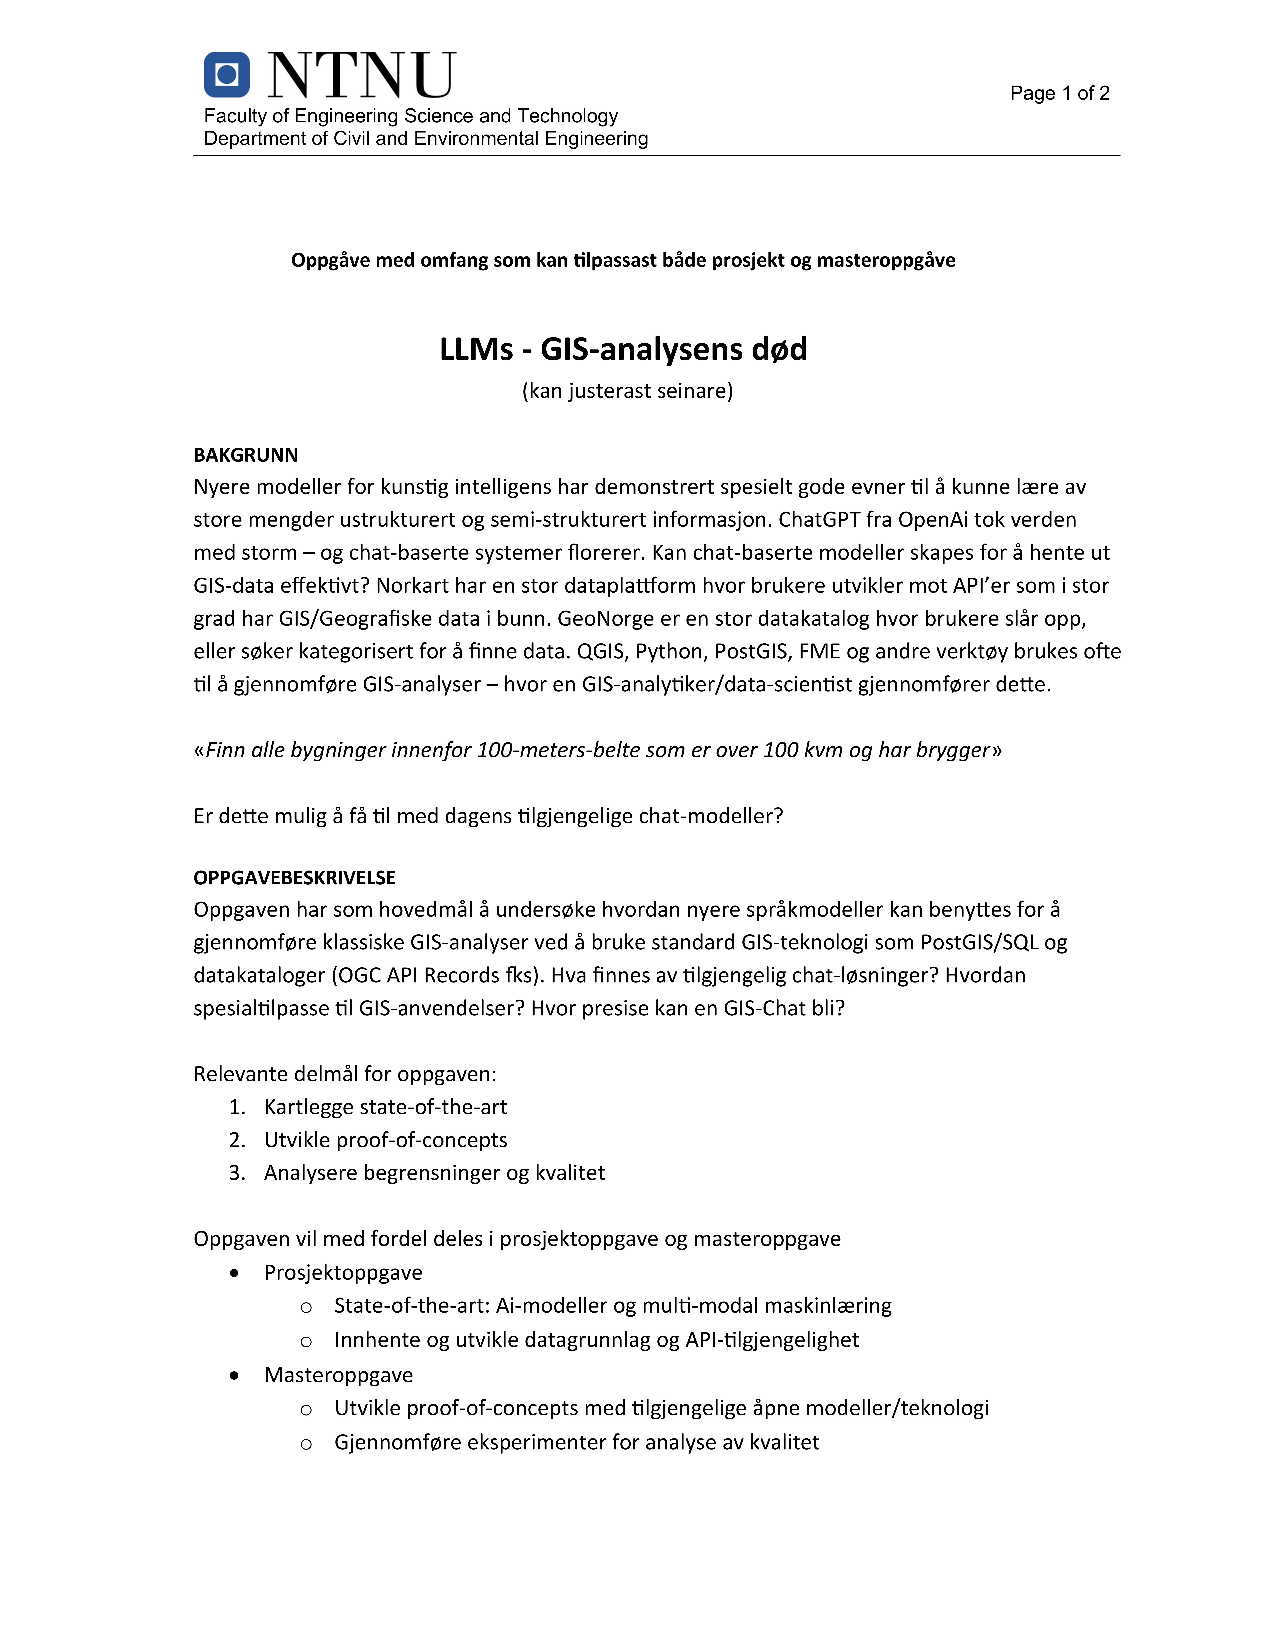
\includepdf[pages=1-, scale=1]{appendices/project_description.pdf}

\addcontentsline{toc}{chapter}{Abstract}    % can be left out
\section*{Abstract}

\begin{comment}
This paper provides a template for writing a Master's Thesis
(parts of it can also be used when writing a Specialisation Project Report).
The template does not form a compulsory style that you are obliged to use, but rather provides a common starting point for all students. For a given thesis, tuning of the template may still be required, depending on the nature of the thesis and the author's writing style.
Such tuning might involve moving a chapter to a section or vice versa, or removing or adding sections and chapters.

    [If you write a Specialisation Project Report, it should normally focus on the background, related work (i.e., your literature study), and future work sections ---
        with the ``future work'' section containing the plan for the Master's Thesis work to be carried out in the second semester.
        Architectural and experimental sections can also be included, but in preliminary versions.
        All those sections should of course be updated in the Master's Thesis and adapted to the actual work carried out.]

Note that the template contains a lot of examples of how to write different parts of the thesis
as well as how to cite authors and how to use LaTeX and BibTeX.
Some of those examples might only be clear if you actually look at the LaTeX source itself.

The abstract is your sales pitch which encourages people to read your work,
but unlike sales it should be realistic with respect to the contributions of the work.
It should include:
\begin{itemize}
    \item the field of research,
    \item a brief motivation for the work,
    \item what the research topic is,
    \item the research approach(es) applied, and
    \item contributions.
\end{itemize}

The abstract length should be roughly half a page of text (and not more than one page).
It will normally be longer than the abstracts you see in research papers, since some more background / motivation is included.
Do not include lists, tables or figures.
Avoid abbreviations and references.

When writing the abstract, keep in mind that most people might only read this text (and many only the title), so be sure to make it sound good.
What you really want to accomplish is that people who read the abstract will get drawn into your project and read the rest of the text too.
However, the old saying most definitely applies here: You never get a second chance to make a first impression.
\end{comment}

The emergence of powerful \glspl{acr:llm} with remarkable reasoning and coding capabilities---like \acrshort{acr:gpt}-4, the latest additions to the \acrshort{acr:gpt} series---enables automation of a wide range of tasks. ChatGPT's Code Interpreter is able to generate, execute, and review its own code, making development of autonomous \acrshort{acr:ai} agents far easier than before. This specialization project report explores the feasibility of \gls{acr:llm}-based \acrshort{acr:gis} agents, investigating how ChatGPT is currently being used in the field of \acrshort{acr:gis}, how such \glspl{acr:llm} could be used if applied in larger systems, and how such systems can be implemented. This report seeks to highlight the strengths of current \gls{acr:llm}-based technologies, but also their weaknesses, and suggest areas of improvements and possible solutions to overcome current limitations. These goals are achieved through a literature study and three experiments that aim to support the findings of the literature study. The literature study presents the body of work that has already been done in regard to the position of \glspl{acr:llm} in the field of \acrshort{acr:gis}, as well as planning strategies applied in \gls{acr:llm}-based agents, and retrieval-augmented generation---that is, giving the \gls{acr:llm} \enquote{hooks} into the real world. The three experiments focus on ChatGPT's ability to handle geospatial data in various formats and through different access channels. The overall goal of this specialisation project is to lay the groundwork for development of \gls{acr:llm}-based \acrshort{acr:gis} agents.

\glsresetall

% \null\newpage

\addcontentsline{toc}{chapter}{Sammendrag}  % can be left out
\begin{otherlanguage}{norsk}

    \section*{Sammendrag}

\end{otherlanguage}

\begin{comment}
Husk at hvis du er en norsk student og skriver masteren din på engelsk, så \textit{må\/} du lage et sammendrag på norsk.
Bruk ikke Google Translate eller lignende, uten skriv teksten direkte på norsk.
Sammendraget trenger absolutt ikke å være identisk ord-for-ord med abstract, men skal selvsagt ha i prinsipp samme innehold, på semantisk nivå.

(If you are a non-Norwegian student, it is not obligatory to include an abstract in Norwegian.)

For those who write a Norwegian summary, whatever you do, do \textit{not\/} just directly translate the English abstract.
It might be tempting to think that the Norwegian summary is something you can do on the fly --- maybe assuming that nobody will read it.
However, in fact the opposite might be true: it is very likely that it will be read by the people you most want to make a good impression on,
such as your friends, family, and future employers.
\end{comment}
% \null\newpage

\addcontentsline{toc}{chapter}{Preface}     % can be left out
\section*{Preface}

\begin{comment}
The Preface includes the facts: what type of project, where it is conducted,
who supervised, and any acknowledgements you wish to give.

This Master's Thesis template was created by Bj\"orn Gamb\"ack and is based on a template that he created for the 2016 ``Experts in Team'' course on
Computational Creativity (TDT4853) at the Norwegian University of Science and Technology (NTNU),
which in turn was heavily based on the 2014 AI Master's Thesis template created by Anders Kofod-Petersen ---
with some of the explaining text stemming from Anders' original template.

You may basically thank anybody you like (and avoid thanking anybody you do not like) and in any form you like.
However, it is a good idea to always thank people who made direct contributions, e.g., those whose data you have been given access to or those whose images you have been given permission to reproduce.

Some students choose to include the text of the original project description in the Preface. This is possible but not necessary,
in particular not if you have changed the theme somewhat over time.
The Preface of the Master's Thesis might also be a good place to introduce your Specialisation Project, in case you plan
on reusing some texts from it (since the Specialisation Project is not a published and easily accessible work, and might
not be known to your audience, neither your text in itself nor even the general concept as such).
\end{comment}

This master's thesis is written at the Norwegian University of Science and Technology, for the Division of Geomatics at the Department of Civil and Environmental Engineering.

I would like to thank Hongchao Fan, my supervisor at the Division of Geomatics, and my two supervisors from Norkart: Alexander Salveson Nossum and Arild Nomeland. I would also like to thank GeoForum and Digin for inviting me to present my thesis at Geomatikkdagene and GeoAI:Konferansen, respectively. Finally, I would like to thank my ever-supporting family for their constant encouragement and support throughout my studies.

\vfill

\hfill \thesisAuthor

\hfill Trondheim, \today

% \null\newpage

\tableofcontents
\clearpage
% \null\newpage

\printglossary[type=\acronymtype]
% \printglossary
\clearpage
% \null\newpage

\listoffigures
\addcontentsline{toc}{chapter}{List of Figures}
\clearpage
% \null\newpage

\listoftables
\addcontentsline{toc}{chapter}{List of Tables}
\clearpage
% \null\newpage

\lstlistoflistings
\addcontentsline{toc}{chapter}{List of Code Snippets}
% \listofcodes
% \clearpage

\glsaddall

%%%%%%%%%%%%%%%%%%%%%%%%%%%%%%%%%%%%%%%%%%%%%%%%%%%%%
\mainmatter

\chapter{Introduction}
\label{cha:introduction}

\begin{comment}
All chapters should begin with an introduction before any sections, giving an overview of the chapter content.
Each section should in addition start with an introduction before its subsections begin.
Chapters with just one section --- or sections with just one sub-section --- should be avoided.
Think carefully about chapter and section titles as each title stands alone in the table of contents (without associated text)
and should convey the meaning of the contents of the chapter or section.

In all chapters and sections it is important to write clearly and concisely. Avoid repetitions and if needed refer back to the original discussion or presentation.
Each new section, subsection or paragraph should provide the reader with new information and be written in your own words. Avoid direct quotes.
If you use direct quotes, unless the quote itself is very significant, you are conveying to the reader that you are unable to express this discussion or fact yourself.
Such direct quotes also break the flow of the language (yours to someone else's).
\end{comment}

The \nameref{cha:introduction} will open with \autoref{sec:background-and-motivation}, explaining the motivation behind this master's thesis. Continuing, \autoref{sec:goals-and-research-questions} will lay out the overarching goals, and formulate three research questions, before \autoref{sec:research-method} explains the research method of the thesis, which is to be considered a technical thesis. \Autosectionref{sec:intro-contributions} will list the main contributions of the work, before \autoref{sec:thesis-structure} gives the reader a high-level overview of the thesis to conclude the \nameref{cha:introduction} chapter.

\section{Background and Motivation}
\label{sec:background-and-motivation}

\begin{comment}
Having a template to work from provides a starting point.
However, for a given project, a slight variation in the template may be required due to the nature of the given project.
Furthermore, the order in which the various chapters and sections will be written will also vary from project to project,
but the writing will seldom start at the abstract and sequentially follow the chapters of the report.
One critical reason for this is that you need to start writing as early as possible and that you will begin to write up where you are currently focusing.
However, do not leave working on the abstract until the very last days. The abstract is the first thing anyone reads of an article or thesis --- after the title;
and thus it is important that it is very well written. Abstracts are hard to write, so create revisions throughout the course of your project.

The background and motivation here should state where your project is situated in the field and what the key driving forces motivating this research are.
However, keep this section brief, as it is still part of the introduction.
The motivation will be further elaborated on in Chapter~\ref{cha:related_work}, presenting your complete state-of-the-art.

Note that this template uses italics to highlight where Latin wording is inserted to represent text and the text of the template
that we wish to draw your attention to. The italics themselves are not an indication that such sections should use italics.

\end{comment}

The release of OpenAI's \textit{ChatGPT} in November, 2022 \citep{openaiIntroducingChatGPT2022} generated a hype within the general population, and chat-based systems are now flourishing. Furthermore, significant advancements have been made within code generation, which makes \acrshortpl{acr:llm} useful for technical tasks, enabling individuals with little to no prior programming experience to carry out computational tasks that require execution of code.

This brings us over to \gls{acr:gis} analysis, which has traditionally been reserved for \acrshort{acr:gis} \textit{experts}. \acrshort{acr:gis} professional are commonly required to know their way around one or more \glspl{acr:gis}, and should preferably be proficient in programming languages suitable for data science tasks, such as Python or R. Sufficient domain knowledge is also necessary when tackling \acrshort{acr:gis} tasks, like knowing what kinds of data to use for a particular task, and where to find them. All of these points, and more, are barriers to entry for people that wish to make use of powerful \acrshort{acr:gis} tools for their own purposes, but lack the technical know-how required to use them correctly. This challenge serves as the overall motivation behind this master's thesis, which will attempt to mitigate these issues by utilizing the vast background knowledge and code generation abilities of modern \glspl{acr:llm}.

\section{Goals and Research Questions}
\label{sec:goals-and-research-questions}

\begin{comment}
A research project needs to have one or several question(s) that should be answered.
It is desirable to formulate such questions as early as possible as they provide both an important driving force for the project and clarity as to the goals sought.
However, expect to refine the questions and thus the final path of the project as work progresses.
Any refinements should be conducted with care, so as to avoid that the original aims and previous work are lost.
It is always good to have one (or max two) research goals and perhaps some subgoals,
together with 2--3 explicit research questions (or max four).

\begin{description}
    \item[Goal] \textit{Lorem ipsum dolor sit amet, consectetur adipiscing elit.}
\end{description}

Your goal/objective should be described in a single sentence.
In the text underneath it you can expand on this sentence to clarify what is meant by the short goal description.
The goal of your work is what you are trying to achieve. This can either be the goal of your actual project or
can be a broader goal that you have taken steps towards achieving. Such steps should be expressed in the research questions.
Note that the goal is seldom to build a system. A system is built to enable experiments to be conducted.
The research goal stages the needs that the system is implemented to meet.

\begin{description}
    \item[Research question 1] \textit{Lorem ipsum dolor sit amet, consectetur adipiscing elit.}
\end{description}

Each research question provides a sub-goal and these should be precise and clearly stated enabling the reader to match your results to the original goals.
They will also form the driving force for the experimental plan.

\begin{description}
    \item[Research question 2] \textit{Lorem ipsum dolor sit amet, consectetur adipiscing elit.}
\end{description}

Potentially, how well the goals have been met (and how well the research questions have been answered)
is a theme that you should return to towards the end of the thesis (so in Chapter~\ref{cha:conclusion} and/or Chapter~\ref{cha:discussion}).

For a Specialisation Project, the goal would primarily be to get up to speed with the research field, so the research questions will rather be
limited to exploring what the state-of-the-art is, what methods and data have been used, etc.
A secondary goal of the specialisation is to frame the research questions and goals of the Master's Thesis.
Note that a major difference between the Specialisation Project and the Master's Thesis is that the Master's Thesis work \textit{has\/} to
introduce new research.
Of course the Specialisation Project can also introduce novel work, but there is no such requirement --- and most commonly it does not,
since the core of the project really is to figure out what is ``old'' before you can introduce something which is new.
\end{comment}

Deriving from the motivation described in the section above, the overarching goal of this master's thesis is to investigate the possibilities of utilizing \glspl{acr:llm} to create a natural language interface with a system that is capable of solving \acrshort{acr:gis}-related tasks. The overall hypothesis is that modern \glspl{acr:llm} possess a sufficient understanding of common \acrshort{acr:gis} workflows which, when paired with their excellent code generation abilities, should enable them to solve a variety of such tasks.

Based on the overarching goal, three research questions have been constructed and are listed below:

\begin{enumerate}
    \item Can an \gls{acr:llm}-based system solve common \acrshort{acr:gis} tasks? \label{rq:gis-question-answering}
    \item What are core challenges in developing \acrshort{acr:llm}-based \acrshortpl{acr:gis}? \label{rq:development-challenges}
    \item Can an \acrshort{acr:llm}-based \acrshort{acr:gis} replace \acrshort{acr:gis} professionals? \label{rq:replaing-gis-professionals}
\end{enumerate}

\section{Research Method}
\label{sec:research-method}

\begin{comment}
What methodology will you apply to address the goals: theoretic/analytic, model/abstraction or design/experiment?
This section will describe the research methodology applied and the reason for this choice of research methodology.
You should return to the actual choices made in the work and the alternatives in the Discussion chapter.
\end{comment}

This master's thesis will be of a technical character, and will revolve around the development of a \enquote{proof of concept}. The usefulness of this \enquote{proof of concept} will be evaluated through a series of tests, which will help answer the research questions listed in \autoref{sec:goals-and-research-questions}. This report will predominantly serve to highlight the contributions of the proof of concept and the experiments, as these activities constituted the bulk of the time spent on the master's thesis.

\section{Contributions}
\label{sec:intro-contributions}

\begin{comment}
This section just provides a brief summary of the main contributions of the work.
The main description of the contributions will come in Section~\ref{sec:contributions}, after the results are presented.
(Hence Section~\ref{sec:introContributions} can also be left out, leaving the discussion completely to Section~\ref{sec:contributions}.)

The format of this section will generally be as follows:

\begin{enumerate}
    \item \textit{Lorem ipsum dolor sit amet, consectetur adipiscing elit.}
    \item \textit{Lorem ipsum dolor sit amet, consectetur adipiscing elit.}
    \item \textit{Lorem ipsum dolor sit amet, consectetur adipiscing elit.}
\end{enumerate}

\noindent
where the items on the list briefly describe the key contributions.

The order of the contributions here is important. List your main contribution first!
Creating this list will help you not only with writing the Conclusion (where all items listed here definitely should be included, and in more detail),
but also with items that need to be mentioned in the Abstract, as well as with points that you will want to bring to attention in the Discussion.
Hence most of the content on this list will be addressed 4--5 times in your text: here, in the Abstract, Discussion, Conclusion, and (most likely)
in the Results chapter.
\end{comment}

Below is a brief description of the contributions of this master's thesis:

\begin{enumerate}
    \item A chat-based \acrshort{acr:gis} named \textit{GeoGPT}, powered by \acrshortpl{acr:llm}, that can perform tasks commonly solved using \acrshort{acr:gis} software.
    \item A new \acrshort{acr:gis} benchmark that will help give insigth into the ability of a system like GeoGPT to solve common \acrshort{acr:gis} tasks when provided only with a natural language problem formulation.
    \item An investigation into the open question of the extent to which GeoGPT can replace \acrshort{acr:gis} professionals.
\end{enumerate}

\section{Thesis Structure}
\label{sec:thesis-structure}

\begin{comment}
This section provides the reader with an overview of what is coming in the next chapters.
You want to say more than what is explicit in the chapter name, if possible, but still keep the description short and to the point. So something along the lines of:

\begin{itemize}
    \item Chapter~\ref{cha:background_theory} introduces the theory, tools and methods necessary to understand the work.
    \item \textit{Lorem ipsum dolor sit amet, consectetur adipiscing elit.}
    \item Chapter~\ref{cha:conclusion} sums up the work and points to ways it can be improved or extended in the future.
\end{itemize}
\end{comment}

Below is an outline of the thesis' structure:

\begin{itemize}
    \item \Autochapterref{cha:background-theory} introduces the theory and tools necessary for the reader to be familiar with in order to understand the rest of the work. It also provides insight into the work that has been done on autonomous, \acrshort{acr:llm}-based systems, particularly within the field of geomatics.
    \item \Autochapterref{cha:architecture} will lay out GeoGPT's architecture, providing both a high-level overview and details on important parts of the system.
    \item \Autochapterref{cha:experiments} presents the experimental setup, the datasets utilized, and the results and evaluations obtained from these experiments.
    \item \Autochapterref{cha:discussion} discusses the experimental results in light of the research questions and addresses additional points of discussion that arise from these results.
    \item \Autochapterref{cha:future-work} suggests potential areas of improvement in GeoGPT that are suitable for future research.
    \item \Autochapterref{cha:conclusion} will conclude the master's thesis, reiterating the main contributions of the work.
\end{itemize}


\glsresetall
\chapter{Background Theory}
%OR: \chapter{Tools and Methods}
\label{cha:background-theory}

\begin{comment}
The background theory depth and breadth depend on the depth needed to understand your project
in the different disciplines that your project crosses.
It is not a place to just write about everything you know that is vaguely connected to your project.
The theory is here to help the readers that do not know the theoretical basis of your work so that they
can gain sufficient understanding to understand your contributions --- and also for yourself to show that
you have understood the underlying theory and are aware of the methods used in the field.
In particular, the theory section provides
an opportunity to introduce terminology that can later be used without disturbing the text with a definition.
In some cases it will be more appropriate to have a separate section for different theories (or even separate chapters).
However, be careful so that you do not end up with too short sections.
Subsections may also be used to separate different background theories.

Be aware that ``background'' is a general term that refers to everything done by somebody else,
in contrast to the ``foreground'', which is your own work.
Hence there can (and will) be several background chapters, with the background theory being one of them
--- or several of them, since it thus is quite possible to split the background theory over more than one chapter,
e.g., by having a chapter introducing the theory directly needed for the research field in question and another
chapter discussing the machine learning theory, algorithms, tools, and evaluation methods commonly used in the field.
The related work chapter is thus also part of the background, while a chapter about data might be background
(if you only use somebody else datasets), but can also be part of the foreground (if you collect and/or annotate data
yourself, or if you process or clean the data in ways that can make it part of your own contribution).

It is ok to reuse material from other texts that you have written (e.g., the specialisation project), but if you do so, that must be clearly stated in the text, together with a description of how much of the text is new, old or rewritten/edited.
Such a statement about recycling of material in the Background Theory chapter can thus come here in the chapter introduction.

\section{Writing References in the Text}
\label{sec:writing_references}

When introducing techniques or results, always reference the source.
Be careful to reference the original contributor of a technique and not just someone who happens to use the technique.%
\footnote{But always make sure that you have read the work you are citing --- if not, cite someone who has!}
For results relevant to your work,
you would want to look particularly at newer results so that you have referenced the most up-to-date work in your area.
A common rule of thumb is to at least reference the first paper introducing the issue and the paper containing the latest / state-of-the-art
results. Additional papers making substantial contributions should also be referenced, as well as of course the ones you find most interesting.
Remember to use the right verb form depending on the number of authors.

If you do not have the source handy when writing, mark in the text that a reference is needed and add it later. \todo{add reference}
Web pages are not reliable sources --- they might be there one day and removed the next; and thus should be avoided, if possible.
A verbal discussion is not a source and should normally not be referenced
(though you can reference ``personal communication'', if there are no other options).
The bulk of citations in the report will appear in Chapter~\ref{cha:related_work}.
However, you will often need to introduce some terminology and key citations already in this chapter.

You can cite a paper in the following manner (and several other versions,
see the \verb!natbib! package documentation):

\begin{enumerate}[(i)]
    \item When referring to authors, using their names in the text:\\
          \citet{Authorson;Bobsen:10} stated something rather nice.
          (using \verb!\citet!)
    \item To cite indirectly: \\
          Papers should be written nicely \citep{Authorson;Bobsen:10}
          (using \verb!\citep!)
          {\em or\/}\\
          In \citet{Authorson;Bobsen:10}, a less detailed template was presented.
    \item To just cite the authors: \\
          \citeauthor{Authorson;Bobsen:10} wrote a nice paper
          (using \verb!\citeauthor!).
    \item Or just the year: \\ \citeyear{Authorson;Bobsen:10}
          (using \verb!\citeyear!).
    \item You can even cite specific pages or chapters: \citet[p. 3]{Authorson;Bobsen:10}
          (using \verb!\citet[...]{...}!).
\end{enumerate}

You should obviously always cite your supervisor's work \citep{BenyonEA:13},
even if it is completely irrelevant \citep{Das;Gamback:13a} or very old \citep{AlshawiEA:91b}.
Digging up an even older book can also appear impressive \citep{Diderichsen:57}.
(Or? ;-)

\section{The Reference List}
\label{sec:reference_list}

In general, make sure that the references that appear in your reference list can be easily located and identified by the reader.
So include not only authors and title, but year and place of publication, the full names of conferences and workshops,
page numbers in proceedings and collections, etc.
Hyperlinks or \acrfull{acr:doi} numbers are also nice to include.
Just as in the text itself, it is important to be consistent in the reference list, so include the same type of information for all references and write it in the same way.

Check out the reference list at the end of this document for examples of how to write references in \BibTeX.
Note a particular quirk: Many \BibTeX\ styles convert uppercase letters to lowercase, unless specifically told not to.
You might thus need to ``protect'' characters that should not be converted, e.g., by writing \texttt{\{T\}witter} as in the \citet{FountaEA:18} reference.

Also, keep in mind that `et' is a word in its own right (`and'), so there is no period after it (even though there is a period after `al.', which is short for `alia', meaning `others').
Of course, when including such a reference in the text, the authors should be referred to in plural form.
So \citet{BenyonEA:13} state that life is good (not ``states'').

Many sites, such as journals and \url{dblp.org} provide the matching \BibTeX\ entry for a reference.
However, you might still need to edit the entry in order to be consistent with the rest of your references.
If you find references from sites such as \url{scholar.google.com} or \url{arXiv.org}, keep in mind that they often not are complete,
so that you might need to add information to the entry (and probably edit it as well).

Some other good sites to find state-of-the-art work:
\begin{itemize}
    \item \url{paperswithcode.com}
    \item \url{nlpprogress.com}

\end{itemize}

\textit{Lorem ipsum dolor sit amet, consectetur adipiscing elit, sed do eiusmod tempor incididunt ut labore et dolore magna aliqua. Ut enim ad minim veniam, quis nostrud exercitation ullamco laboris nisi ut aliquip ex ea commodo consequat. Duis aute irure dolor in reprehenderit in voluptate velit esse cillum dolore eu fugiat nulla pariatur. Excepteur sint occaecat cupidatat non proident, sunt in culpa qui officia deserunt mollit anim id est laborum.}

\begin{figure}[t!]
    \centering
    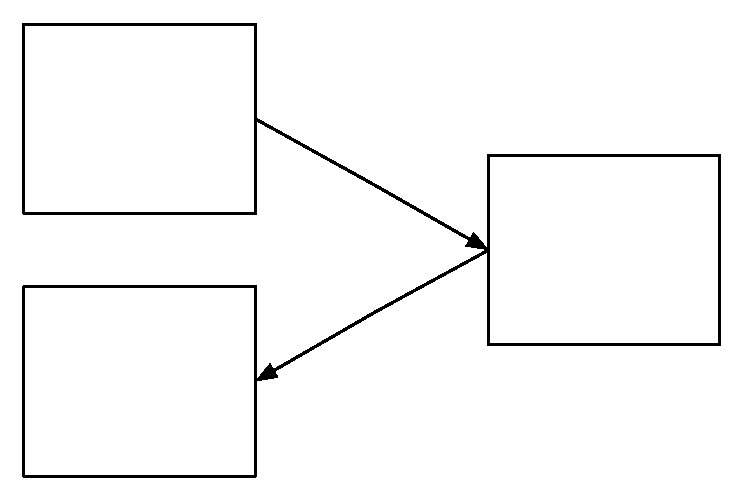
\includegraphics[width=0.5\columnwidth]{figs/figure1.pdf}
    \caption[Boxes and arrows are nice]{Boxes and arrows are nice (adapted from \citealp{Authorson;Bobsen:10}, reprinted with permission)}
    \label{fig:BoxesAndArrowsAreNice}
\end{figure}

\section{Introducing Figures}

\LaTeX is a bit tricky when it comes to the placement of ``flooting bodies'' such as figures and tables. It is often a good idea to let their code appear right before the header of the (sub)section in which they appear.
Note that you should anyhow always use an option for the placement (e.g., \verb|[t!]| to place it at the top of a page).

Remember that if you reproduce someone else's figures you must credit the original author --- such as
Figure~\ref{fig:BoxesAndArrowsAreNice} (adapted from \citealp{Authorson;Bobsen:10}),
as well as state that you have permission to reprint it (e.g., if it is published under a Creative Commons License,
or if you have gained explicit permission from the author).

Do not just put the figure in and leave it to the reader to try to understand what the figure is.
The figure should be included to convey a message and you need to help the reader to understand the message
intended by explaining the figure in the text.
Hence \textbf{all} figures and tables should always be referenced in the text, using the \verb!\ref! command.
It is good practice to always combine it with a non-breakable space (\verb!~!) so that there will be no newline between the term referring to it and the reference, that is, using \verb!Figure~\ref{fig:BoxesAndArrowsAreNice}!.

If a figure appears far from the text explaining it,
it is a good idea to add its page number (using the \verb!\pageref! command), so that you can refer to Figure~\ref{fig:BoxesAndArrowsAreNice} (on Page~\pageref{fig:BoxesAndArrowsAreNice}).

Also, note that you can have a longer version of the figure (and table) caption attached to the actual figure,
while using the optional first argument to \verb!\caption! to include a shorter version in the list of figures (lof) or list of tables:
\begin{quote}
    \begin{verbatim}
\caption[Shorter lof text]{Longer text appearing under the figure}
\end{verbatim}
\end{quote}

It is good practice to add a note about a missing figure in the text,
such as the completely amazing stuff that will appear in Figure~\ref{fig:AmazingFigure}.

\begin{figure}[t!]
    \centering
    \missingfigure{Here we will add an amazing figure explaining it all}
    \caption{A missing figure}
    \label{fig:AmazingFigure}
\end{figure}

In general it is good to add notes about things that you plan on writing later.
The \verb!todonotes! package is great for that kind of book-keeping, letting you write both shorter comments in the margin\todo{l8r dude} and longer comments inside the text, using the option \verb![inline]!.
\todo[inline]{There are always some more stuff that you will need to add at some later point.
    Be sure to at least make a note about it somewhere.}

\textit{Sed ut perspiciatis unde omnis iste natus error sit voluptatem accusantium doloremque laudantium, totam rem aperiam, eaque ipsa quae ab illo inventore veritatis et quasi architecto beatae vitae dicta sunt explicabo. Nemo enim ipsam voluptatem quia voluptas sit aspernatur aut odit aut fugit, sed quia consequuntur magni dolores eos qui ratione voluptatem sequi nesciunt. Neque porro quisquam est, qui dolorem ipsum quia dolor sit amet, consectetur, adipisci velit, sed quia non numquam eius modi tempora incidunt ut.}

\section{Introducing Tables in the Report}

\newcommand\emc{-~~~~}
\begin{table}[t!]
    \centering
    \caption[Example table]{Example table (F$_1$-scores); this table uses the optional shorter caption that will appear in the list of tables, so this long explanatory text will not appear in the list of tables and is only here in order to explain that to the reader.}
    \begin{tabular}{c|c|rrrrrr}
        \tabletop
        Langs                  & Source                                           & \multicolumn{1}{c}{Lang1} & \multicolumn{1}{c}{Lang2} & \multicolumn{1}{c}{Univ} & \multicolumn{1}{c}{NE} & \multicolumn{1}{c}{Mixed} & \multicolumn{1}{c}{Undef}
        \\ \tablemid
        \multirow{5}{*}{EN-HI} & FB+TW                                            & 54.22                     & 22.00                     & 19.70                    & 4.00                   & 0.05                      & 0.03                      \\
                               & FB                                               & 75.61                     & 4.17                      & 18.00                    & 2.19                   & 0.02                      & 0.01                      \\
                               & TW                                               & 22.24                     & 48.48                     & 22.42                    & 6.71                   & 0.08                      & 0.07                      \\
                               & Vyas                                             & 54.67                     & 45.27                     & 0.06                     & \emc                   & \emc                      & \emc                      \\
                               & FIRE                                             & 45.57                     & 39.87                     & 14.52                    & \emc                   & 0.04                      & \emc                      \\ \tablemid
        \multirow{2}{*}{EN-BN} & TW                                               & 55.00                     & 23.60                     & 19.04                    & 2.36                   & \emc                      & \emc                      \\
                               & FIRE                                             & 32.47                     & 67.53                     & \emc                     & \emc                   & \emc                      & \emc                      \\ \tablemid
        EN-GU                  & FIRE                                             & 5.01                      & \textbf{94.99}            & \emc                     & \emc                   & \emc                      & \emc                      \\
        \tablemid
        DU-TR                  & Nguyen                                           & 41.50                     & 36.98                     & 21.52                    & \emc                   & \emc                      & \emc                      \\ \tablemid

        EN-ES                  & \multirow{4}{*}{\rotatebox[origin=c]{90}{EMNLP}}
                               & 54.79                                            & 23.50                     & 19.35                     & 2.08                     & 0.04                   & 0.24                                                  \\
        EN-ZH                  &                                                  & 69.50                     & 13.95                     & 5.88                     & 10.60                  & 0.07                      & \emc                      \\
        EN-NE                  &                                                  & 31.14                     & 41.56                     & 24.41                    & 2.73                   & 0.08                      & 0.08                      \\
        AR-AR                  &                                                  & 66.32                     & 13.65                     & 7.29                     & 11.83                  & 0.01                      & 0.90                      \\ \tablebot
    \end{tabular}
    \label{tab:ExampleTable}
\end{table}

As you can see from Table~\ref{tab:ExampleTable}, tables are nice.
However, again, you need to discuss the contents of the table in the text.
You do not need to describe every entry, but draw the reader's attention to what is important in the table,
e.g., that 94.99 is an amazing F$_1$-score (and that probably something fishy happened there).
Use boldface, boxes, colours, arrows, etc. to mark the important parts of the table.

As can be seen in the example, elements in a table can sometimes benefit from being rotated (such as EMNLP in the `Source' column) or cover more than one row (EMNLP, as well as EN-HI and EN-BN in the `Langs' column) --- or more than one column, for that matter.

\textit{Donec non turpis nec neque egestas faucibus nec id neque. Etiam consectetur, odio vitae gravida tempus, diam velit sagittis turpis, a molestie ligula tellus at nunc. Proin dolor neque, dapibus a pellentesque a, commodo a nibh.}
\end{comment}

\begin{itshape}
    NB! Parts of the \nameref{cha:background-theory} chapter is reused material from the specialization project \citep{holmLLMsDeathGIS2023} preceding this master thesis. Below are the sections in question, together with a description of the extent to which, and how, the material is reused:

    \begin{itemize}
        \item \Autosubsectionref{subsec:attention-and-the-transformer-architecture}: Reused without modification.
        \item \Autosubsectionref{subsec:sota-llms}: \acrshort{acr:gpt} part reused without modification.
    \end{itemize}
\end{itshape}

\vspace{12pt}

\noindent \Autochapterref{cha:background-theory} will lay a theoretical basis for the work done in this master thesis, providing the user with the required understanding in order to understand the contributions of the work. \Autosectionref{sec:language-modelling} will explain the theoretical basis of the component which most modern \glspl{acr:llm} are based upon --- namely the Transformer --- and the attention mechanism within it. The section will also touch upon a new approach to language modelling called \textit{selective state space modelling}, which has yielded very promising results for small \glspl{acr:llm}.


\section{Approaches to Language Modelling}
\label{sec:language-modelling}

\Autosubsectionref{subsec:attention-and-the-transformer-architecture} will explain the theoretical basis behind most modern \glspl{acr:llm}, which are based upon the attention mechanism built into the Transformer architecture. \Autosubsectionref{subsec:state-space-models} will explain modern state space-modelling approaches and why they may have a potential greater than Transformer-based models. First, however, \autoref{subsec:statistical-models-and-rnns} will delve into earlier attempts at language modelling.

\subsection[Early Attempts: Statistical Models and Recurrent Neural Networks]{Early Attempts: Statistical Models and \acrlongpl{acr:rnn}}
\label{subsec:statistical-models-and-rnns}

\subsection{Statistical Models}


\subsection[Recurrent Neural Networks]{\acrlongpl{acr:rnn}}


\subsection{Attention and the Transformer Architecture}
\label{subsec:attention-and-the-transformer-architecture}


\cite{vaswaniAttentionAllYou2017} managed to achieve new state-of-the-art results for machine translation tasks with their introduction of the Transformer architecture. The Transformer has later been proved effective for numerous downstream tasks, and for a variety of modalities. Titling their paper \citetitle{vaswaniAttentionAllYou2017}, \citeauthor{vaswaniAttentionAllYou2017} suggest that their attention-based architecture renders network architectures like \glspl{acr:rnn} redundant, due to its superior parallelization abilities and the shorter path between combinations of position input and output sequences, making it easier to learn long-range dependencies \citep[6]{vaswaniAttentionAllYou2017}.

The Transformer employs self-attention, which enables the model to draw connections between arbitrary parts of a given sequence, bypassing the long-range dependency issue commonly found with \glspl{acr:rnn}. An attention function maps a query and a set of key-value pairs to an output, calculating the compatibility between a query and a corresponding key \citep[3]{vaswaniAttentionAllYou2017}. Looking at \citeauthor{vaswaniAttentionAllYou2017}'s proposed attention function \eqref{eq:attention}, we observe that it takes the dot product between the query $Q$ and the keys $K$, where $Q$ is the token that we want to compare all the keys to. Keys similar to $Q$ will get a higher score, i.e., be \textit{more attended to}. These differences in attention are further emphasized by applying the softmax function. The final matrix multiplication with the values $V$ (the initial embeddings of the input tokens) will yield a new embedding in which all individual tokens have some context from all other tokens. We improve the attention mechanism by multiplying queries, keys, and values with weight matrices that are learned through backpropagation. Self-attention is a special kind of attention in which queries, keys, and values are all the same sequence.

\begin{equation}
    \text{Attention}(Q, K, V) = \text{softmax}\left(\frac{QK^T}{\sqrt{d_k}}\right)V
    \label{eq:attention}
\end{equation}

Attention blocks can be found in three places in the Transformer architecture \citep[5]{vaswaniAttentionAllYou2017} (I will use machine translation from Norwegian to German as an example):

\begin{enumerate}
    \item In the encoder block to perform self-attention on the input sequence (which is in Norwegian)
    \item In the decoder block to perform self-attention on the output sequence (which is in German)
    \item In the decoder block to perform cross-attention (also known as encoder-decoder attention) where each position in the decoder attends to all positions in the encoder
\end{enumerate}

The Transformer represented a breakthrough in the field of \gls{acr:nlp}, and is the fundamental building block of modern \glspl{acr:llm}, most famous of which are the \acrshort{acr:gpt}'s.

\subsection{State Space Models}
\label{subsec:state-space-models}


\section[Large Language Models]{\acrlongpl{acr:llm}}

\subsection[Function Calling LLMs]{Function Calling \acrshortpl{acr:llm}}
\label{subsec:function-calling}

\textit{Function calling} --- first introduced by OpenAI \citep{eletiFunctionCallingOther2023} --- allows developers to provide function definitions to an \gls{acr:llm} and have said \gls{acr:llm} output a \acrshort{acr:json} object containing the name of one or more of the functions provided, as well as suitable arguments to these. Made possible through fine-tuning models to detect when functions should be calling, function calling makes it possible to give an \gls{acr:llm} \textit{hooks} into the real world, and provides a more reliable way for developers to integrate \glspl{acr:llm} into applications.

Possible use cases include using functions provide correct and up-to-date information that would otherwise require extensive training and fine-tuning. Having the \gls{acr:llm} use function calling for information retrieval also make them more transparent, making it possible to trace a claim back to its source, something that is normally a difficult feat with \gls{acr:llm}. Another use case might be code execution. One could imagine a rather simple function \texttt{execute\_python\_code(code: string) -> string} that takes Python code as a string and returns the standard output that results from executing that code. This is likely the principle behind products like OpenAI's Data Analysis mode (previously Code Interpreter), in which ChatGPT functions as a code executing agent that can generate, execute, and self-correct its own code. Similar functions could be constructed for \acrshort{acr:sql}, making it possible for \glspl{acr:llm} to work against relational databases. As \cite{eletiFunctionCallingOther2023} describes, function calling can also be used to extract structured data from text.

\subsection[State-of-the-Art Models]{State-of-the-Art \acrlongpl{acr:llm}}
\label{subsec:sota-llms}

\subsubsection{The GPT Family}
\label{subusubsec:gpt}

\gls{acr:gpt} is a type of \gls{acr:llm} that was introduced by OpenAI in 2018 \citep{radfordImprovingLanguageUnderstanding2018}. Specifically designed for text generation, a \acrshort{acr:gpt} is essentially a stack of Transformer \textit{decoders}. It demonstrates through its vast pre-training on unlabelled data that such unsupervised training can help a language model learn good representations, providing a significant performance boost while alleviating the dependence on supervised learning. While the original Transformer architecture as described by \cite{vaswaniAttentionAllYou2017} was intended for machine translation---thus having encoders to learn the representation of the origin language representation of a given input sequence and decoders to learn the representation in the target language and perform cross-attention between the two---the \acrshort{acr:gpt} is designed only to \textit{imitate} language. This is why there are no encoders to be found in the \acrshort{acr:gpt} architecture, only decoders. The model employs masked multi-head attention (running the input sequence through multiple attention heads in parallel), and is restricted to only see the last $k$ tokens---with $k$ being the size of the context window---and tasked to predict the next one.

Training consists of two stages: unsupervised pre-training and supervised fine-tuning. The former is used to find a good initialization point, essentially teaching the model to imitate the corpora upon which it is trained. This results in a model that will ramble on uncontrollably, just trying to elaborate upon the input sequence it's given to the best of its knowledge. This will naturally produce undefined behaviour, and it is therefore necessary to fine-tune the model on target tasks in a supervised manner. \cite[4]{radfordImprovingLanguageUnderstanding2018} explain how the model can be fine-tuned directly on tasks like text classification, but how one for other tasks needs to convert structured inputs into ordered sequences because the pre-trained model was trained on contiguous sequences of text. In the case of ChatGPT, \citeauthor{openaiIntroducingChatGPT2022} used \gls{acr:rlhf} by employing a three-step strategy: first training using a supervised policy, then using trained reward models to rank alternative completions produced by ChatGPT models, before fine-tuning the model using \gls{acr:ppo}, which is a way of training \acrshort{acr:ai} policies. This pipeline is then performed for several iterations until the model produces the desired behaviour \citep{openaiIntroducingChatGPT2022}.

\subsubsection{The Gemini Family}
\label{subsubsec:gemini}

\subsubsection{The Claude Family}
\label{subsubsec:claude}

\subsubsection{Open-Source Alternatives}
\label{subsubsec:open-source-llms}


\section{LangChain}
\label{sec:langchain}

LangChain \citep{langchainaiLangchainaiLangchain2022} is an open-source project that provides tooling which simplifies the way developers interface with \glspl{acr:llm}. This tooling includes composable tools and integrations that can be used to build prompts for \acrshortpl{acr:llm}, as well as off-the-shelf chains that perform higher level tasks. Chains are \glspl{acr:dag} --- or sequences of runnables --- that take an input and produces and output. A runnable can be a prompt template with template literals that are substituted with values that are passed into the runnable. The output is the template with the template literals filled in. This output can then be chained into an \acrshort{acr:llm} runnable calls a language model using the prompt template. The output from the \acrshort{acr:llm} runnable could then be passed into an output parser, e.g. a \acrshort{acr:json} parser, that ensures that the chain outputs a \acrshort{acr:json} object. Such chains are the buildings blocks that make up LangChain.

Common use cases for LangChain are:

\begin{itemize}
    \item Building chatbots for question answering that use semantic retrieval from document store
    \item Creating agents with access to external tools be leveraging function calling (see \autoref{subsec:function-calling})
    \item Creating code executing agents for Python, \acrshort{acr:sql}, or other programming languages
\end{itemize}

In January 2024, LangChain AI rolled out a new framework called LangGraph which builds on top of the LangChain ecosystem. While the chains commonly found in LangChain are good for \gls{acr:dag} workflow, they are not suited to creating cyclic graphs. LangGraph can be used to add cycles to \acrshort{acr:llm} applications, which are important for agent-like behaviours \citep{langchainaiLangchainaiLanggraph2024}. A graph in LangGraph is a set of nodes that pass some state around, state that can be modified by each node. The nodes are connected together by edges that define what node can succeed another node. These edges can also be conditional, which routes execution to a given node based on the output from a function giving the current state. This allows for complex logic and simplifies implementation of advanced agent patterns, some of which are discussed in \autoref{sec:agent-patterns}.


\section{Geospatial Databases and Data Catalogues}
\label{sec:geo-dbs-and-data-catalogues}

This section will discuss the geospatial technologies that were used or considered for use in this master's thesis.

\subsection{PostGIS}

PostGIS \citep{PostGIS2001} is an open-source extension for the PostgreSQL \acrshort{acr:dbms}.

\subsection[OGC API Features]{\acrshort{acr:ogc} \acrshort{acr:api} Features}

\acrshort{acr:ogc} \acrshort{acr:api} Features \citep{opengeospatialconsortiumOGCAPIFeatures2022} is an \acrshort{acr:api} specification that defines modular \acrshort{acr:api} building blocks for interacting with features, real-world objects. These building blocks include blocks for creating, modifying, and querying features on the Web. A typical implementation of \acrshort{acr:ogc} \acrshort{acr:api} Features implements these building blocks for \acrshort{acr:html}, GeoJSON, and \acrshort{acr:gml}. These are called \textit{requirement classes}, though none of them are strictly required. The \acrshort{acr:html} requirement class gives the user of the \acrshort{acr:api} a visualization of the features, whereas the GeoJSON and \acrshort{acr:gml} requirements classes are typically meant for use in other applications.

\begin{figure}[h]
    \centering
    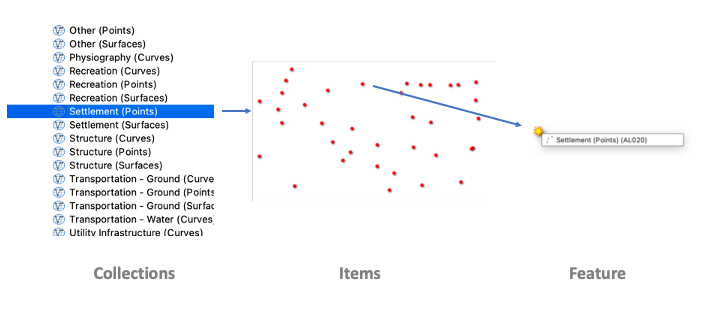
\includegraphics[width=\textwidth]{ogc_api_features.png}
    \caption{Collections, items, and features in \acrshort{acr:ogc} \acrshort{acr:api} Features specification. Retrieved from \url{https://features.developer.ogc.org/} April 29th 2024.}
    \label{fig:oaf-collections-items-features}
\end{figure}

\subsection[SpatioTemporal Asset Catalogs]{\acrlong{acr:stac}}










\glsresetall

% \chapter{Related Work}
\label{cha:related_work}

\begin{comment}
What other research has been conducted in this area and how is it related to your work?
This section is thus where your literature review will be presented. It is important when presenting the review
that you give an overview of the motivating elements of the work going on in your field and how these relate to your work,
rather than a list of contributors and what they have done.
This means that you need to extract the key important factors for your work and discuss how others have addressed
each of these factors and what the advantages/disadvantages are with such approaches.
As you mention other authors, you should reference their work.
Note that the reference list reflects the literature you have read {\em and\/} have cited.
This will only be a subset of the literature that you have read.

A good way to find relevant work is by checking what others are referencing, e.g., in papers you have already found
or in previous studies carried out at NTNU, such as \cite{Berg;Gopinathan:17}.
However, when doing that,
do not fall into one of the common traps, such as re-iterating someone's false quote or faulty analysis of
a previous paper (check the original source!), or getting stuck inside a local research cluster (a group of
researchers that mainly refer to the ones using the same type of approaches or similar ideas).

Make sure that it is clear how and why you decided to include some references (and discard others). As in all parts of research, it should ideally be possible for someone else to reproduce your work, also when it comes to finding the relevant references.
There are (at least) three basic methods for finding references:
\begin{enumerate}
    \item Trust the authorities (e.g., your supervisor) to dig out good texts for you.
          Those can often be used as a seed set for:
    \item Snowballing, where you have some good articles and check the references in them for other good ones.
          Note that this can be done both backwards and forwards on the timeline; that is, using tools like Google Scholar, you can also check who refers \textit{to\/} the good articles you have already found.
    \item Carry out a Systematic Literature Review (or Structured Literature Review, SLR), a method introduced more formally into Software Engineering by \citet{Kitchenham;Charters:07}, but based on several similar methods for other disciplines.
          At the core of the method is an SQL-related  search over a reference database (such as Google Scholar).
          A good introduction to SLR is given by \citet{Kofod-Petersen:14}.
\end{enumerate}

Note that a reference needs to be complete: you should always give the full name of a conference or journal,
always include page numbers, always say where a book or thesis was published, and where a conference took place, as further described in Section~\ref{sec:reference_list}.

Just as described in the Background chapter (Chapter~\ref{cha:background_theory}), it is possible (and even likely) that you will want to reuse some of the text that you have written for your specialisation project in your Master's Thesis.
This is allowed, as long as it is clearly stated what you have reused and in what form (e.g., if a section is a straight-forward copy, if it has undergone only editorial changes, if it contains some old material but also some new, etc.).
\end{comment}

\glsresetall 
% \chapter{Datasets}
% OR: \chapter{Data}
\label{cha:data}

\begin{comment}
You will (probably) need to describe and discuss the dataset(s) that you use in your work.
Depending on how much detail is needed and whether you have done any work on the data yourself
(including analysing it, collecting or annotating some of it, or cleaning/preprocessing it),
the data description can possibly be part of the Background chapter, the Related Work chapter,
the Architecture chapter or the Experimental Setup.
The dataset(s) can also be described in a separate chapter, either before or after the chapter on related work.
Note that if you have put some effort of your own into the data, you will need to make sure that the text about it
is part of the ``foreground'' (your own work) rather than the ``background'' (everything done by somebody else), which includes the theoretical
background chapter(s) and the related work.

\textit{Lorem ipsum dolor sit amet, consectetur adipiscing elit. Phasellus pulvinar tempor enim eu hendrerit. Integer consequat ipsum ac erat malesuada, et aliquet dolor gravida. Sed pulvinar vehicula risus id sagittis. Nulla ut nisi ligula. Vestibulum ante ipsum primis in faucibus orci luctus et ultrices posuere cubilia curae; Nullam viverra elit magna, eget interdum enim placerat sed. Duis iaculis non sapien vel tincidunt. Aliquam malesuada molestie mauris ac congue. Nam sit amet felis ex. Nulla convallis tempor lacus eget accumsan. Phasellus arcu velit, pharetra in dolor at, commodo volutpat leo. Praesent nec purus quam. In dignissim vitae sem nec euismod. Maecenas sed feugiat nunc. Cras blandit condimentum libero. Aenean quis efficitur sem.}

\textit{Duis lobortis, mauris a maximus consectetur, sem est interdum justo, eget varius orci augue a tellus. Vestibulum vehicula erat eu eros dignissim, non rhoncus lorem commodo. Mauris et leo vel urna feugiat ornare a ac dolor. Etiam faucibus velit vitae pellentesque ultrices. Pellentesque habitant morbi tristique senectus et netus et malesuada fames ac turpis egestas. Donec facilisis in enim nec fermentum. Vestibulum ante ipsum primis in faucibus orci luctus et ultrices posuere cubilia curae;}

\textit{Maecenas ullamcorper et purus vel facilisis. Pellentesque habitant morbi tristique senectus et netus et malesuada fames ac turpis egestas. Aenean eget diam elit. Vestibulum dolor nunc, porttitor eget porta in, mollis at neque. Phasellus nec tempus diam, non scelerisque orci. Sed tincidunt, lorem a bibendum vehicula, nulla nunc vulputate purus, non viverra sem enim nec est. Aliquam erat volutpat. Praesent in sem tortor. Sed fringilla a nisl et dictum. Nullam faucibus venenatis diam, in sodales magna auctor vel. Suspendisse ornare turpis pulvinar nibh venenatis vulputate.}

\textit{Aliquam eget vulputate tellus. Suspendisse viverra eros sem, eu dapibus diam finibus a. Aenean at lectus eget mi convallis rutrum ut sit amet elit. Curabitur nec nisl mauris. Nullam finibus, elit et vehicula posuere, ante ipsum tristique massa, vitae dictum lorem quam eu est.}

\begin{table}[t!]
    \centering
    \begin{tabular}{l|cccc|c}
        \tabletop
        Dataset   & Normal & Offensive & Hateful & Spam    & Total           \\
        \tablemid
        Original  & 53,790 & 27,037    & 4,948   & 14,024  & \textbf{99,799} \\
        Available & 41,784 & 14,202    & 2,941   & ~~9,372 & \textbf{68,299} \\
        \tablebot
    \end{tabular}
    \caption[The \citeauthor{FountaEA:18} dataset]{The original \citet{FountaEA:18} dataset vs its availability in 2020, given by \citeauthor{Isaksen;Gamback:20}}
    \label{tab:data}
\end{table}

You probably  want a table giving some statistics regarding the data.
As an example, Table~\ref{tab:data} shows a common problem when working with Twitter (X) data:
the authors of a dataset may only provide tweet IDs that other researches can use to retrieve tweets through the Twitter \gls{api};
however, some tweets may for several reasons not be retrievable later on, e.g., since a tweet or the user account behind a tweet may have been deleted.
Here, of $99,799$ tweet IDs provided by \citet{FountaEA:18}, only $68,299$ tweets could actually be retrieved two years later,
as described by \citet{Isaksen;Gamback:20}.

\textit{Morbi viverra ante et tortor faucibus finibus nec sit amet sem. In ultrices, augue sed vestibulum congue, tortor turpis sodales odio, at interdum leo justo non massa. Nunc aliquet, nisl non vestibulum rhoncus, libero tortor laoreet nibh, vel ultricies nunc erat nec nisl. Praesent sed lorem arcu. Sed ultricies, tellus at euismod posuere, felis nibh cursus justo, vitae placerat nisl lorem ut est. Suspendisse sollicitudin sagittis nibh, ac interdum erat hendrerit id. Fusce est mi, semper eget mauris sed, posuere ultrices orci. Aenean nec est eu augue blandit maximus. Morbi ut nisl at metus condimentum tincidunt nec consectetur nibh. Phasellus eleifend dapibus elit ut cursus. Donec lacinia turpis a justo dignissim, sit amet venenatis libero pellentesque. Orci varius natoque penatibus et magnis dis parturient montes, nascetur ridiculus mus.}
\end{comment}

With the interest of investigating the ability of a \gls{acr:llm}-based system to perform geospatial analysis, relevant datasets should be accessible to said system. \Autosectionref{sec:data-sources} provides a description of the datasets used in the experiments. Furthermore, it was decided to explore different access channels to this data. \Autosectionref{sec:data-access} elaborates on this.

\section{Data Sources}
\label{sec:data-sources}

\begin{comment}
A total of eight datasets were used in the experiments. All datasets were downloaded through Geonorge\footnote{\url{https://geonorge.no}}, a webpage administered by The Norwegian Mapping Authority that serves as a portal to a large catalogue of Norwegian geographical data. The datasets were selected to provide a diverse pool of geographical data to perform analysis upon. \autoref{tbl:datasets} shows the datasets used along with a description.


\begin{table}[htbp]
    \centering
    \caption{Datasets used in experiments}
    \label{tbl:datasets}
    \begin{tabularx}{\textwidth}{p{3cm}|X}
        \toprule
        \textbf{Dataset}                          & \textbf{Description}                                                                                                                                                                                                                                                                              \\
        \midrule
        AR50 - Land Use Map                       & A nationwide dataset that displays main types of land use adapted for use in scales from 1:20,000 to 1:100,000.                                                                                                                                                                                   \\
        \midrule
        Strategic Noise Mapping from Road Traffic & The strategic noise mapping shows the noise situation from road traffic at the turn of the year 2016/2017 for the largest urban areas in the country and in addition along national and county roads where more than 8,200 vehicles pass per day.                                                 \\
        \midrule
        Elveg 2.0 - Road Network                  & A road network dataset that includes all drivable roads that are longer than 50 meters, or part of a network, as well as pedestrian and bicycle paths and bicycle paths represented as road link geometry.                                                                                        \\
        \midrule
        Cadastrial Register - Building Points     & The Matrikkelen-Building point dataset contains a small excerpt of the building information registered in the Matrikkelen, Norway's official register of real property, including buildings. The dataset contains representation points, building type, building number, current building status. \\
        \midrule
        Outdoor Recreation Areas                  & The purpose of the dataset is to provide an overview of areas that are important for the public's outdoor life, and it should be easy to account for which assessments and criteria have been the basis for the work and the final product.                                                       \\
        \midrule
        Cultural Monuments - Protected Buildings  & Buildings and churches that are automatically, decision, regulation, or temporarily protected under law and churches that have the status as listed.                                                                                                                                              \\
        \midrule
        Flood Zones                               & Flood zones show areas that are flooded by different flood sizes (recurrence interval). Flood zones are prepared for 20-, 200-, and 1000-year floods.                                                                                                                                             \\
        \midrule
        Quick Clay Zones                          & Provides an overview of zones with potential danger (precautionary areas) for major quick clay landslides.                                                                                                                                                                                        \\
        \bottomrule
    \end{tabularx}
\end{table}

\end{comment}

A total of eighteen datasets were used in the experiments. The data was downloaded from Geofabrik's website\footnote{\url{https://download.geofabrik.de/europe/norway.html}}. Geofabrik --- German for \enquote{geo factory} --- is a company that \enquote{extract, select, and process free geodata}. They have gathered data from OpenStreetMap and published them as a collection of shapefiles, dividing them into categories such as \enquote{places of worship}, \enquote{points of interest}, and \enquote{traffic}. Data can be downloaded for different regions of the world, and for experiments conducted in this thesis, data for Norway was used. \autoref{tbl:datasets} lists all datasets used, along with a short description of their contents. Common for all datasets are their \emph{fclass} attribute, which is short for \emph{feature class}. Some datasets have additional attributes, such as the \emph{maxspeed} attribute in the road data and the \emph{type} attribute in the building data.

\begin{longtable}{p{3cm}p{2.3cm}p{8cm}}
    \caption{Datasets used in experiments}                                                                                                                                                                                        \\
    \label{tbl:datasets}                                                                                                                                                                                                          \\
    \toprule
    \textbf{Dataset}   & \textbf{Data Type} & \textbf{Description}                                                                                                                                                                \\
    \midrule
    \endfirsthead

    \multicolumn{3}{c}%
    {{\bfseries Table \thetable\ continued from previous page}}                                                                                                                                                                   \\
    \toprule
    \textbf{Dataset}   & \textbf{Data Type} & \textbf{Description}                                                                                                                                                                \\
    \midrule
    \endhead

    \midrule
    \multicolumn{3}{r}{{Continued on next page}}                                                                                                                                                                                  \\
    \endfoot

    \bottomrule
    \endlastfoot

    Buildings          & Polygon            & Contains building outlines. Its \emph{type} attribute can have values like \emph{house}, \emph{university}, and \emph{restaurant}.                                                  \\
    Land Use           & Polygon            & Represents areas designated to different purposes and activities. Its \emph{fclass} attribute can have values like \emph{forest}, \emph{farmland}, and \emph{residential}.          \\
    Natural            & Point              & Contains outlines of various objects found in nature. Its \emph{fclass} attribute can have values like \emph{beach}, \emph{glacier}, and \emph{cave\_entrance}.                     \\
    Natural            & Polygon            & Similar to the point data equivalent.                                                                                                                                               \\
    Places of Worship  & Point              & Common values for \emph{fclass} attribute: \emph{christian}, \emph{buddhist}, and \emph{muslim}.                                                                                    \\
    Places of Worship  & Polygon            & Similar to the point data equivalent.                                                                                                                                               \\
    Places             & Point              & Common values for \emph{fclass} attribute: \emph{farm}, \emph{village}, and \emph{island}. Repeated entries trimmed for brevity.                                                    \\
    Places             & Polygon            & Similar to the point data equivalent.                                                                                                                                               \\
    Points of Interest & Point              & Common values for \emph{fclass} attribute: \emph{tourist\_info}, \emph{bench}, and \emph{kindergarten}.                                                                             \\                                                                                                                                        \\
    Points of Interest & Polygon            & Similar to the point data equivalent.                                                                                                                                               \\
    Railways           & Lines              & Common values for \emph{fclass} attribute: \emph{rail}, \emph{subway}, and \emph{tram}. Also has True/False attributes saying if a given line segment is a bridge or a tunnel.      \\
    Roads              & Lines              & Common values for \emph{fclass} attribute: \emph{rail}, \emph{subway}, and \emph{tram}. Has additional attributes \emph{oneway}, \emph{maxspeed}, \emph{bridge}, and \emph{tunnel}. \\
    Traffic            & Point              & Common values for \emph{fclass} attribute: \emph{crossing}, \emph{street\_lamp}, and \emph{parking}.                                                                                \\
    Traffic            & Polygon            & Common values for \emph{fclass} attribute: \emph{parking}, \emph{pier}, and \emph{dam}.                                                                                             \\
    Transport          & Point              & Common values for \emph{fclass} attribute: \emph{bus\_stop}, \emph{ferry\_terminal}, and \emph{railway\_station}.                                                                   \\
    Transport          & Polygon            & Similar to the point data equivalent.                                                                                                                                               \\
    Water              & Polygon            & Common values for \emph{fclass} attribute: \emph{water}, \emph{wetland}, and \emph{river\_bank}.                                                                                    \\
    Waterways          & Lines              & Common values for \emph{fclass} attribute: \emph{stream}, \emph{river}, and \emph{canal}.                                                                                           \\
\end{longtable}

\section{Data Access}
\label{sec:data-access}

While leading \glspl{acr:llm} are trained on increasingly large corpora, they are still only as familiar with a topic as the extent to which the training data exposes it to said topic. For instance, many \glspl{acr:llm} are trained specifically to generate Python code, and are therefore fed with a vast number of Python code examples during training in the hopes of improving its performance on benchmarks like \todo{Insert Python benchmark examples here}. As it is unlikely that the training data is evenly distributed among many different topics, it is useful to get familiarized with a model's capabilities in the areas of interest for a particular use case. In the case of an \acrshort{acr:llm}-powered \acrshort{acr:gis} agent that should be capable of performing geospatial analyses, it is useful to know what data formats such an agent is most comfortable to understand and work with.

The upcoming experiments therefore seek to benchmark model performance on three different data access methods. The datasets from \autoref{sec:data-sources} are presented to the model in three different ways, as \autoref{subsec:files} through \autoref{subsec:sql-db} elaborate upon.

\subsection{Files}
\label{subsec:files}

The first method of presentation is to have the files from \autoref{sec:data-sources} remain untouched. The datasets were stored such that each dataset has its own folder. This is because some of the file types used require multiple files in order to correctly store the data—--for instance, the shapefile format, which has three mandatory files: .shp, which contains the actual feature geometry; .shx, which provides a positional index of the feature geometry; and .dbf, which holds attributes for each shape.\todo{reference}

\subsection[SQL Database]{\acrshort{acr:sql} Database}
\label{subsec:sql-db}

The second method used is to load the data into a spatial \acrshort{acr:sql} database and provide the model with database schemas that can be used to generate queries. The datasets were uploaded to a dockerized PostGIS database using QGIS's DB Manager plugin.

Some of the datasets come in the \acrshort{acr:gml} data format, which can include multiple layers with potentially different geometries. For this reason, they cannot be loaded directly into a PostGIS database such that they are stored in the same database table. Furthermore, several of the layers in the multi-layer \acrshort{acr:gml} files are irrelevant for most analysis situations. For instance, the flood zone data were downloaded as a multi-layer \acrshort{acr:gml} file and includes a total of eight layers: polygon and multi-line border for the analysis area, polygon layers for rivers, ocean surfaces, and lakes, polygon and multi-line border for the flood zones, and a layer containing cross-sectional profile lines for the rivers. The quick clay dataset was similar. For brevity, a decision was made not to load all these layers into the PostGIS database. Only the polygon for the flood zones and two polygon layers from the quick clay dataset were loaded into the database.

\subsection[OGC API Features]{\acrshort{acr:ogc} \acrshort{acr:api} Features}
\label{subsec:ogc-api-features-data}

The third method for data access is to use the \acrshort{acr:ogc} \acrshort{acr:api} Features standard.

\glsresetall

\chapter{Architecture}
% OR: \chapter{Model}
\label{cha:architecture}

\begin{comment}
Here you will present the architecture or model that you have chosen and which is (or will be) implemented in your work.
Note that putting algorithms in your report is not always desirable, so in certain cases those might be placed in the appendix.
Code is normally to be avoided in the report itself, but may be included in an appendix or submitted as additional documents.
(The actual code must also be submitted together with the final Master's thesis, but as a zip-file.)

Any off-the-shelf tools and methods that you use in your architecture should have been introduced earlier,
tentatively in the Background chapter (or in the Related Work chapter),
so that they can be referenced here by giving backward pointers to the previous text.

Here, or in a separate chapter (or possibly in the Background chapter or in the Experimental Setup),
you should also discuss the data that you use in your experiments (see Chapter~\ref{cha:data}).

\textit{Nunc in tristique risus, ut malesuada tortor. Integer ullamcorper nunc a felis vehicula condimentum. Aliquam eget turpis purus. Nam nec ipsum sed ligula vulputate tempor ac non arcu. Aenean hendrerit pretium ante et suscipit. Proin vitae venenatis ex, at pellentesque erat. Nulla facilisi. Sed quis eros lorem. Praesent id pharetra risus. Nunc a lacinia est. Nunc in urna at purus ullamcorper blandit eget sit amet est. Cras sagittis et ante ut lobortis. Proin quis arcu eros. Aliquam tempor neque vehicula lacus placerat, ac ultricies massa ultricies. Aliquam et nulla eget felis accumsan rutrum quis sed ligula.}

\textit{Vivamus bibendum tempus tincidunt. Integer imperdiet lectus pellentesque, rhoncus quam at, tempor ex. Phasellus semper tempor sapien at consequat. Proin ut dolor interdum, ullamcorper leo ac, convallis metus. Nullam tincidunt, metus ullamcorper sodales placerat, ipsum ipsum porttitor est, id volutpat orci orci sit amet quam. Vestibulum sagittis urna sit amet nulla vulputate, nec pellentesque enim hendrerit. Suspendisse at laoreet ipsum. Phasellus arcu nisi, laoreet sed tellus sit amet, imperdiet fringilla ante. Quisque rhoncus accumsan magna vel posuere. Fusce facilisis est eros, ac viverra diam maximus ut. Nullam ut lectus nunc. Fusce vestibulum sem at ex euismod tempus. Lorem ipsum dolor sit amet, consectetur adipiscing.}

\textit{Phasellus sed ipsum nunc. Nam iaculis felis mauris, sit amet condimentum ex malesuada at. Morbi lacinia odio mi, sit amet pellentesque ante facilisis sit amet. In lobortis elit ut dictum mollis. Aliquam erat volutpat. Morbi sit amet metus nisi. Nulla auctor varius metus at rhoncus. Pellentesque porta mollis leo, eu ultricies nulla mollis ac. Vivamus interdum ac odio vitae sodales. Aenean finibus eros rhoncus molestie elementum. Integer maximus erat vitae purus lobortis iaculis. Etiam blandit varius nulla, sed euismod felis.}

Clearly, a figure showing the architecture is a must, such as Figure~\ref{fig:Architecture}.
Describe all parts of such a figure in reasonable detail in the text, possibly with forward pointers to sections where they will be elaborated on (or backward pointers to sections where tools and methods already have been introduced).
Mention work that motivated your architectural choices, parameter settings, etc.
Those choices should then also be discussed and elaborated on in the Discussion chapter.

\begin{figure}[t!]
    \centering
    \missingfigure{Architecture figure to be added}
    \caption{The missing architecture}
    \label{fig:Architecture}
\end{figure}
\end{comment}

\section{High-Level Application Architecture}

A microservice architecture was employed in order to simplify development and separate concerns between the different microservices. The services are deployed as Docker Containers, and they are orchestrated using Docker Compose. \todo{quickly explain docker and why it is useful here} \autoref{fig:architecture-overview} shows how the application is divided into five distinct services, and the direction of information flow between these.

\begin{figure}[h]
    \centering
    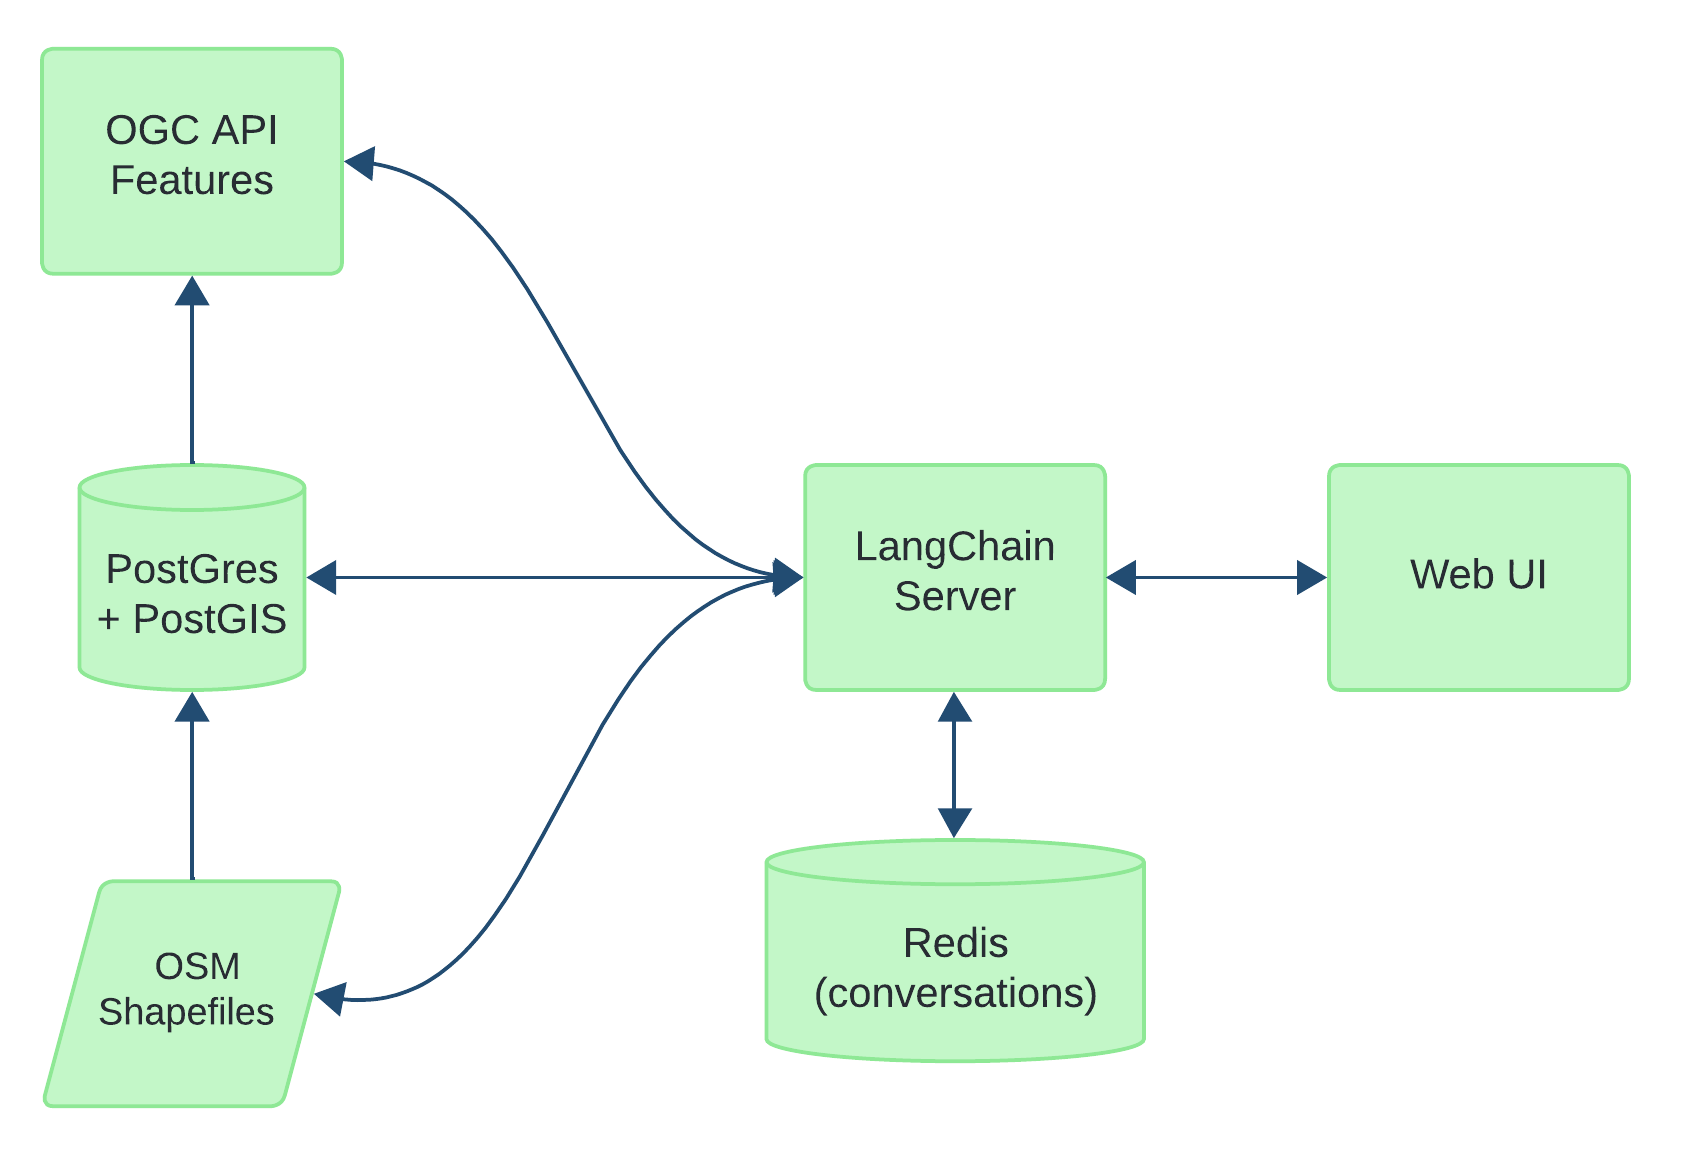
\includegraphics[width=\textwidth]{microservices.png}
    \caption{Architecture overview}
    \label{fig:architecture-overview}
\end{figure}



\subsection{LangChain Server}\label{subsec:langchain}

The \textit{LangChain Server} service is the heart of the application, and is where the \gls{acr:llm}-related logic is situated. It is responsible for taking requests from the \textit{Web \acrshort{acr:ui}} and returning suitable responses in what becomes a client-server architecture between the two services. \autoref{tbl:server-endpoints} show the endpoints exposed by the server and how they can be used by a client.

\begin{table}[h]
    \centering
    \caption{Summary of Server Endpoints}
    \label{tbl:server-endpoints}
    \begin{tabular}{p{0.22\textwidth}p{0.1\textwidth}p{0.55\textwidth}}
        \toprule
        \textbf{Endpoint} & \textbf{Method} & \textbf{Description}                                                                                                                                                         \\
        \midrule
        /session          & GET             & Takes a \texttt{session\_id} as a query parameter, allowing the client to continue on a pre-existing session.                                                                \\
        /session          & POST            & Creates a new session with an empty conversation.                                                                                                                            \\
        /streaming-chat   & GET             & Endpoint for chatting the \acrshort{acr:llm}. Takes a \texttt{message} as a query parameter and returns an event stream, allowing for token streaming from server to client. \\
        /update-map-state & POST            & Send the state of the client map to the server. Keeps the server updated on what layers are present in the map, their color, etc.                                            \\
        /geojson          & GET             & Takes a \texttt{geojson\_path} as a query parameter. Allows the client to retrieve a given GeoJSON file that is stored in the working directory on the server.               \\
        /history          & GET             & Used to retrieve the chat history of the current session.                                                                                                                    \\
        /upload           & POST            & Allows the client to upload one or more files to the working directory on the server.                                                                                        \\
        \bottomrule
    \end{tabular}
\end{table}


\subsection{Redis for Conversations}

Redis \citep{sanfilippoRedisRealtimeData2009} is a fast in-memory database that is often applied as a caching database that sits on top of some persistent database. It can also be used for vector-based storage and as a simple NoSQL database. The latter option is the way it is used in GeoGPT's architecture, and its only purpose is to store conversations. Whenever a user starts a conversation with GeoGPT an object with a unique session ID is stored to the Redis database. This object holds an array that represents the conversation. This array is written to every time either the human or GeoGPT produces a message.

Storing messages --- either in memory as a simple array or in a database like Redis --- is crucial to enable multi-message conversations. In order for a \gls{acr:llm} to act as a conversational agent, some sort of chat history needs to be prepended to the prompt. In the case of GeoGPT the entire chat history is prepended. This has the advantage of providing the \gls{acr:llm} with the complete context of the chat history, but the disadvantage of potentially bloating the context window from which it is supposed to generate tokens. Therefore, as the chat becomes longer each new token will be both more expensive and take more time to get generated. A long chat history could also make the resulting prompt exceed the token limit of the \gls{acr:llm}, or it could confuse model by providing it with messages no longer relevant to the conversation. These issue was not considered in great detail for this project, and are left for future work.

\subsection[PostGIS and OGC API Features]{PostGIS \acrshort{acr:ogc} \acrshort{acr:api} Features}

A PostgreSQL database with the PostGIS extension containing \gls{acr:osm} data was deployed using Docker. On top of this database is a RESTful geospatial feature server called \textit{pg\_featureserv} \citep{crunchydataCrunchyDataPg_featureserv2024}. The web server is realized through the \texttt{pramsey/pg\_featureserv} Docker image\footnote{\url{https://hub.docker.com/r/pramsey/pg_featureserv}}, which is simply passed a database connection string to the database one wishes to expose on the \acrshort{acr:api}. Any tables in that database which have a geometry column and a specified \gls{acr:crs} will be exposed through the web server. pg\_featuresserv allows for features like bounding box filtering, feature limiting, and \acrshort{acr:cql} filtering. These are added as query parameters to the URL of the collection items (for instance: \texttt{.../collections/\{collection\_id\}/items.json?limit=1000\&filter=name IS NOT NULL}). In the internals of pg\_featuresserv, this URL will be converted to an \acrshort{acr:sql} query that will be run against the database. Results of the query will be returned as GeoJSON. \autoref{code:cql-to-sql} shows an example of how \acrshort{acr:cql} code is converted into \acrshort{acr:sql} code:

\begin{lstlisting}[
    language=SQL,
    label=code:cql-to-sql,
    caption=Conversion from \acrshort{acr:cql} to \acrshort{acr:sql}
]
\\ CQL code passed through the `filter` query parameter
within(geom, POINT(0 0))

\\ SQL code that will be run agains the database
ST_Within("geom",'SRID=4326;POINT(0 0)'::geometry)
\end{lstlisting}

\subsection[Web UI]{Web \acrshort{acr:ui}}

The user interface is made with SolidJS. By design, it is very minimal. One of the goals of the project is to simplify the way we do \acrshort{acr:gis} analysis. One of the key design goals was therefore to make the interface as familiar to the user as possible and lowering the chance of the user doing something wrong.

\begin{figure}[h]
    \centering
    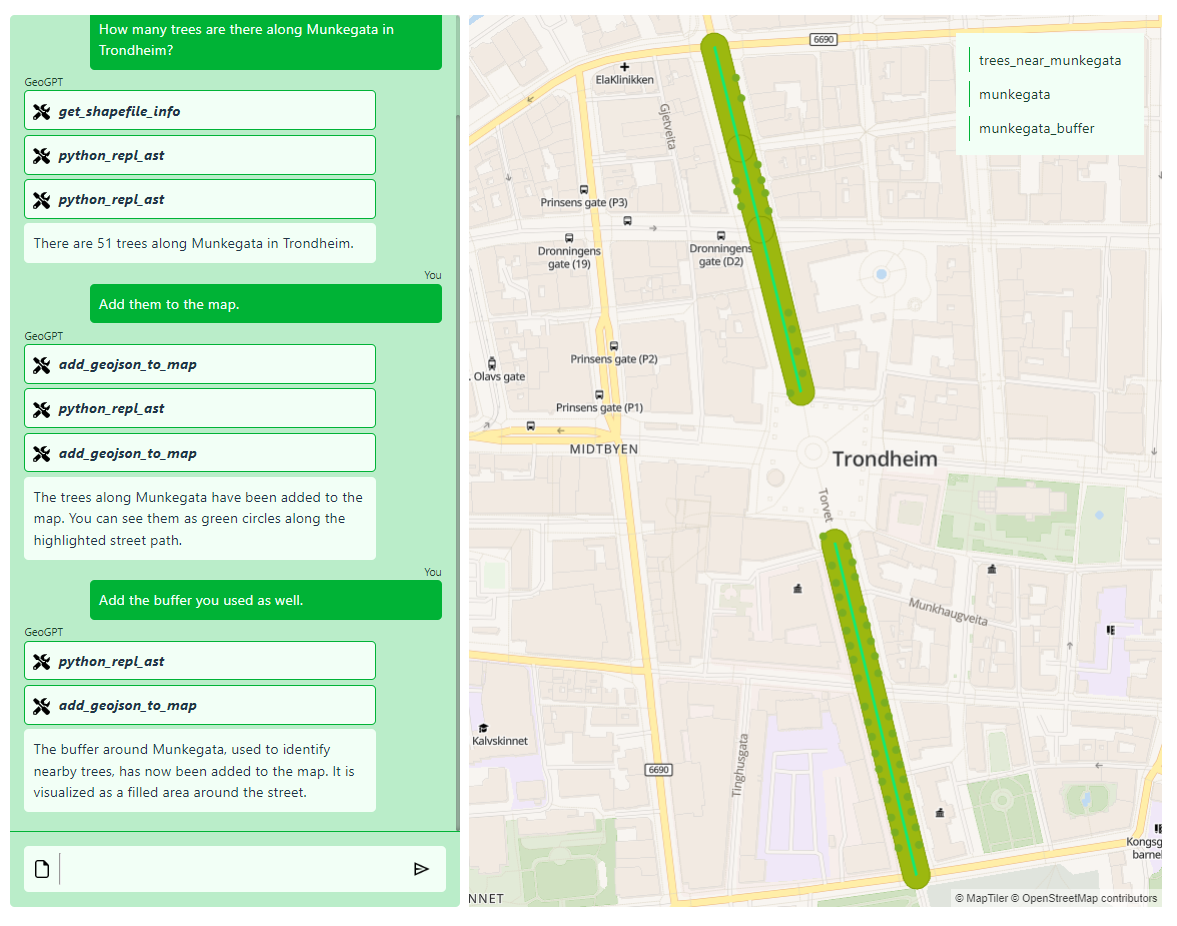
\includegraphics[width=\textwidth]{num_trees_along_munkegata_python_with_buffer.png}
    \caption{Web \acrshort{acr:ui}}
    \label{fig:web-ui}
\end{figure}

The chat interface was designed to imitate the interface of OpenAI's ChatGPT. Tokens and tool messages are streamed from the LangChain server, which helps the user follow the process that GeoGPT goes through when solving a problem. During this process it is possible for the user to cancel token generation if he/she sees that the system is heading off in the wrong direction. The text that is generated and streamed to the client is in Markdown format. A library called \textit{showdown}\footnote{\url{https://github.com/showdownjs/showdown}} is used to convert Markdown into \acrshort{acr:html}, ensuring that tables, code blocks, lists, and other elements are properly rendered. Next to the input field on the bottom of the chat is a file upload button. Files that are uploaded here will be added to the working directory on the LangChain server, allowing GeoGPT to perform analyses on them and optionally adding them to the map.

The map is created using MapLibre\footnote{\url{https://github.com/maplibre/maplibre-gl-js}}, an open-source fork of Mapbox which in December 2020 changed to a non-open-source software licence. A base map from \gls{acr:osm} is used, fetched through a website called MapTiler. GeoJSON files of any kind that are fetched from the server will be added to the map automatically with a random color. On the top-right of the map is an overlay listing all layers that are currently present in the map. Using the arrow keys on this list will change the z-index in the map of the selected layer.



\section{Agent Architecture}

Three different agent were implemented for GeoGPT: one agent utilizing \acrshort{acr:ogc} \acrshort{acr:api} Features, one agent which can access shapefiles using Python code, and one agent that can interact with data in an \acrshort{acr:sql} database. Common to these agents is their agentic architecture, which is described in \autoref{subsec:lg-agent-implementation}. They way that they differ is through their assigned \textit{tools}. These differences will be made apparent in \autoref{fig:tool-agent-graph}. Other slight differences are seen in the way that they are prompted. The prompting strategy used in GeoGPT and these minor differences will be discussed in \autoref{subsec:prompt-templating}.

\subsection{LangGraph Agent Implementation}
\label{subsec:lg-agent-implementation}

The agentic behaviour of GeoGPT is implemented using LangGraph, an extension to LangChain intended to make implementation of cyclic behaviour easier. \autoref{fig:tool-agent-graph} illustrates the flow between the various nodes that make up the agent. A state dictionary is passed between and updated by these nodes. Included in this state is the chat history (previous messages), the path to GeoGPT's working directory, a list of the current files in this directory, and other, less important state. The implementation is based upon a prebuilt implementation from LangGraph.\footnote{\url{https://github.com/langchain-ai/langgraph/blob/main/langgraph/prebuilt/chat_agent_executor.py}}

The \textit{\_\_start\_\_} node serves as the entry point of the agent. At this point, only one message is present in the state, namely the initial message from the user. The \textit{\_\_start\_\_} node points to the \textit{agent} node, where a response to the user is generated by an \acrshort{acr:llm}. This response could contain a textual response, or it could contain instructions to execute some tool. For this reason, the current state containing both the user message and the \acrshort{acr:ai} message, is sent to the \textit{conditional} node called \textit{agent\_should\_continue}. This node simply checks if the agent outcome (the last \acrshort{acr:ai} message) includes the \enquote{tool\_calls} keyword argument. If this is the case then some tool should be executed, and we should \enquote{continue}. If not, the agent has generated a final textual response to the user.

In the \textit{action} node the values inside the \enquote{tool\_calls} object are converted into \texttt{ToolInvocation} objects that are used to invoke predefined tools. \enquote{tool\_calls} is a list of \enquote{tool\_call} objects, each of which has attributes called \textit{name} (the name of the tool) and \textit{arguments} (arguments that should be passed to the tool). These tools are then executed, possibly having side effects on the server, and the resulting output of the tools are appended as messages to the chat history. \autoref{fig:chat-trace-example} illustrates this behavour. This way the agent can inspect the results of the code it is \enquote{executing}, as well as being notified about possible errors in the input parameters it provided. Through the cyclic behaviour of the agent graph the agent can repeatedly call tools to try and answer the request from the user. When the agent finds to reason to call any more tools it generates a textual response, making \textit{agent\_should\_continue} return \texttt{False} so that the termination node (\textit{\_\_end\_\_}) is reached.

\begin{figure}[h]
    \centering
    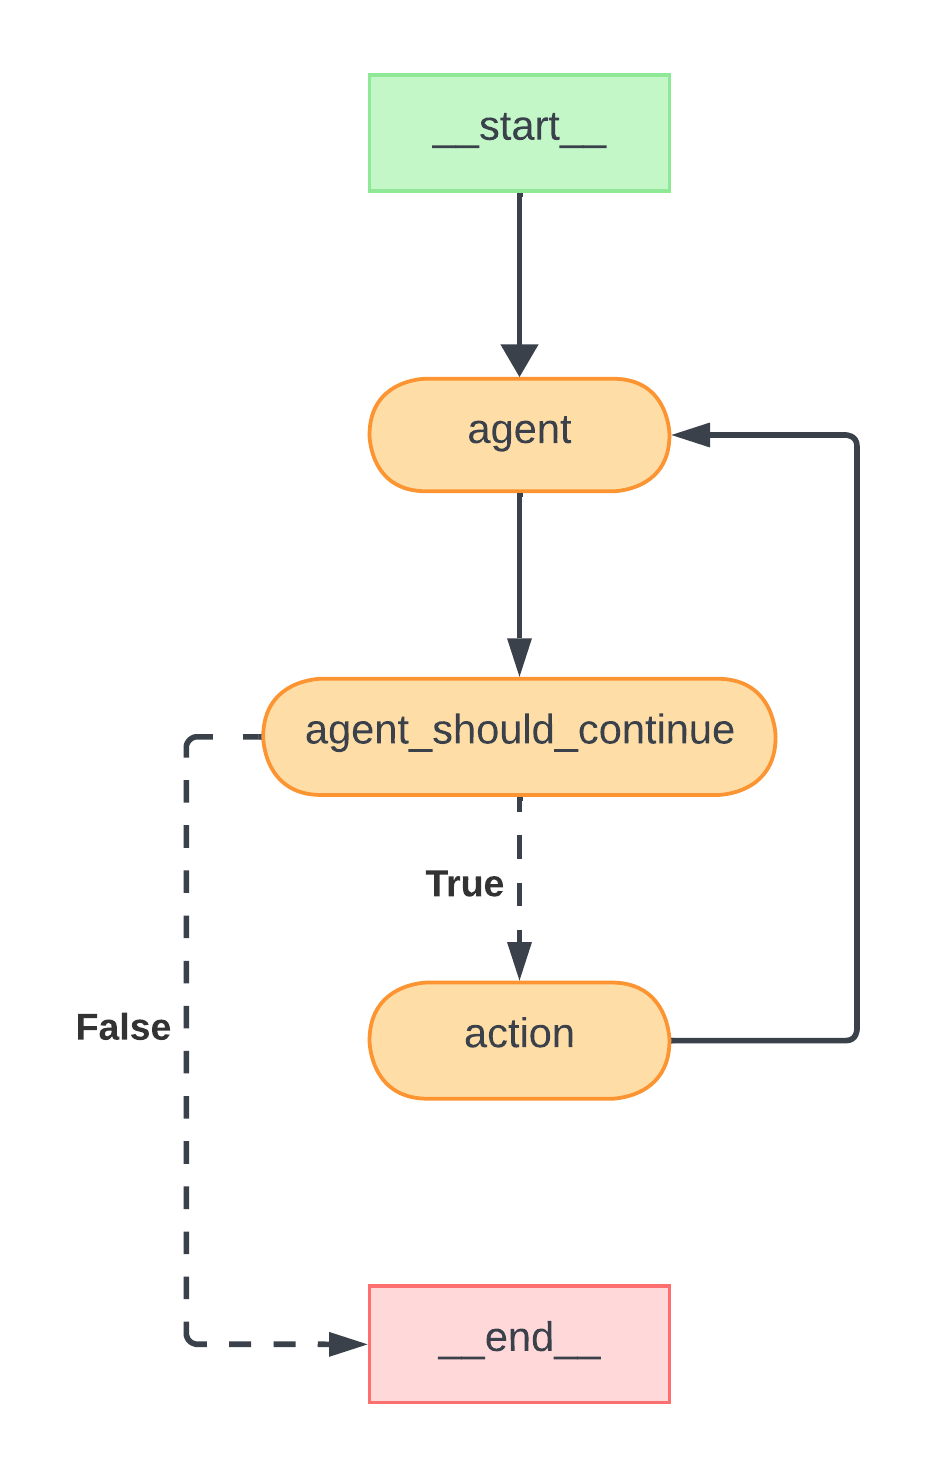
\includegraphics[width=0.6\textwidth]{agent_graph.png}
    \caption{Generic tool agent graph}
    \label{fig:tool-agent-graph}
\end{figure}

\begin{figure}[h]
    \centering
    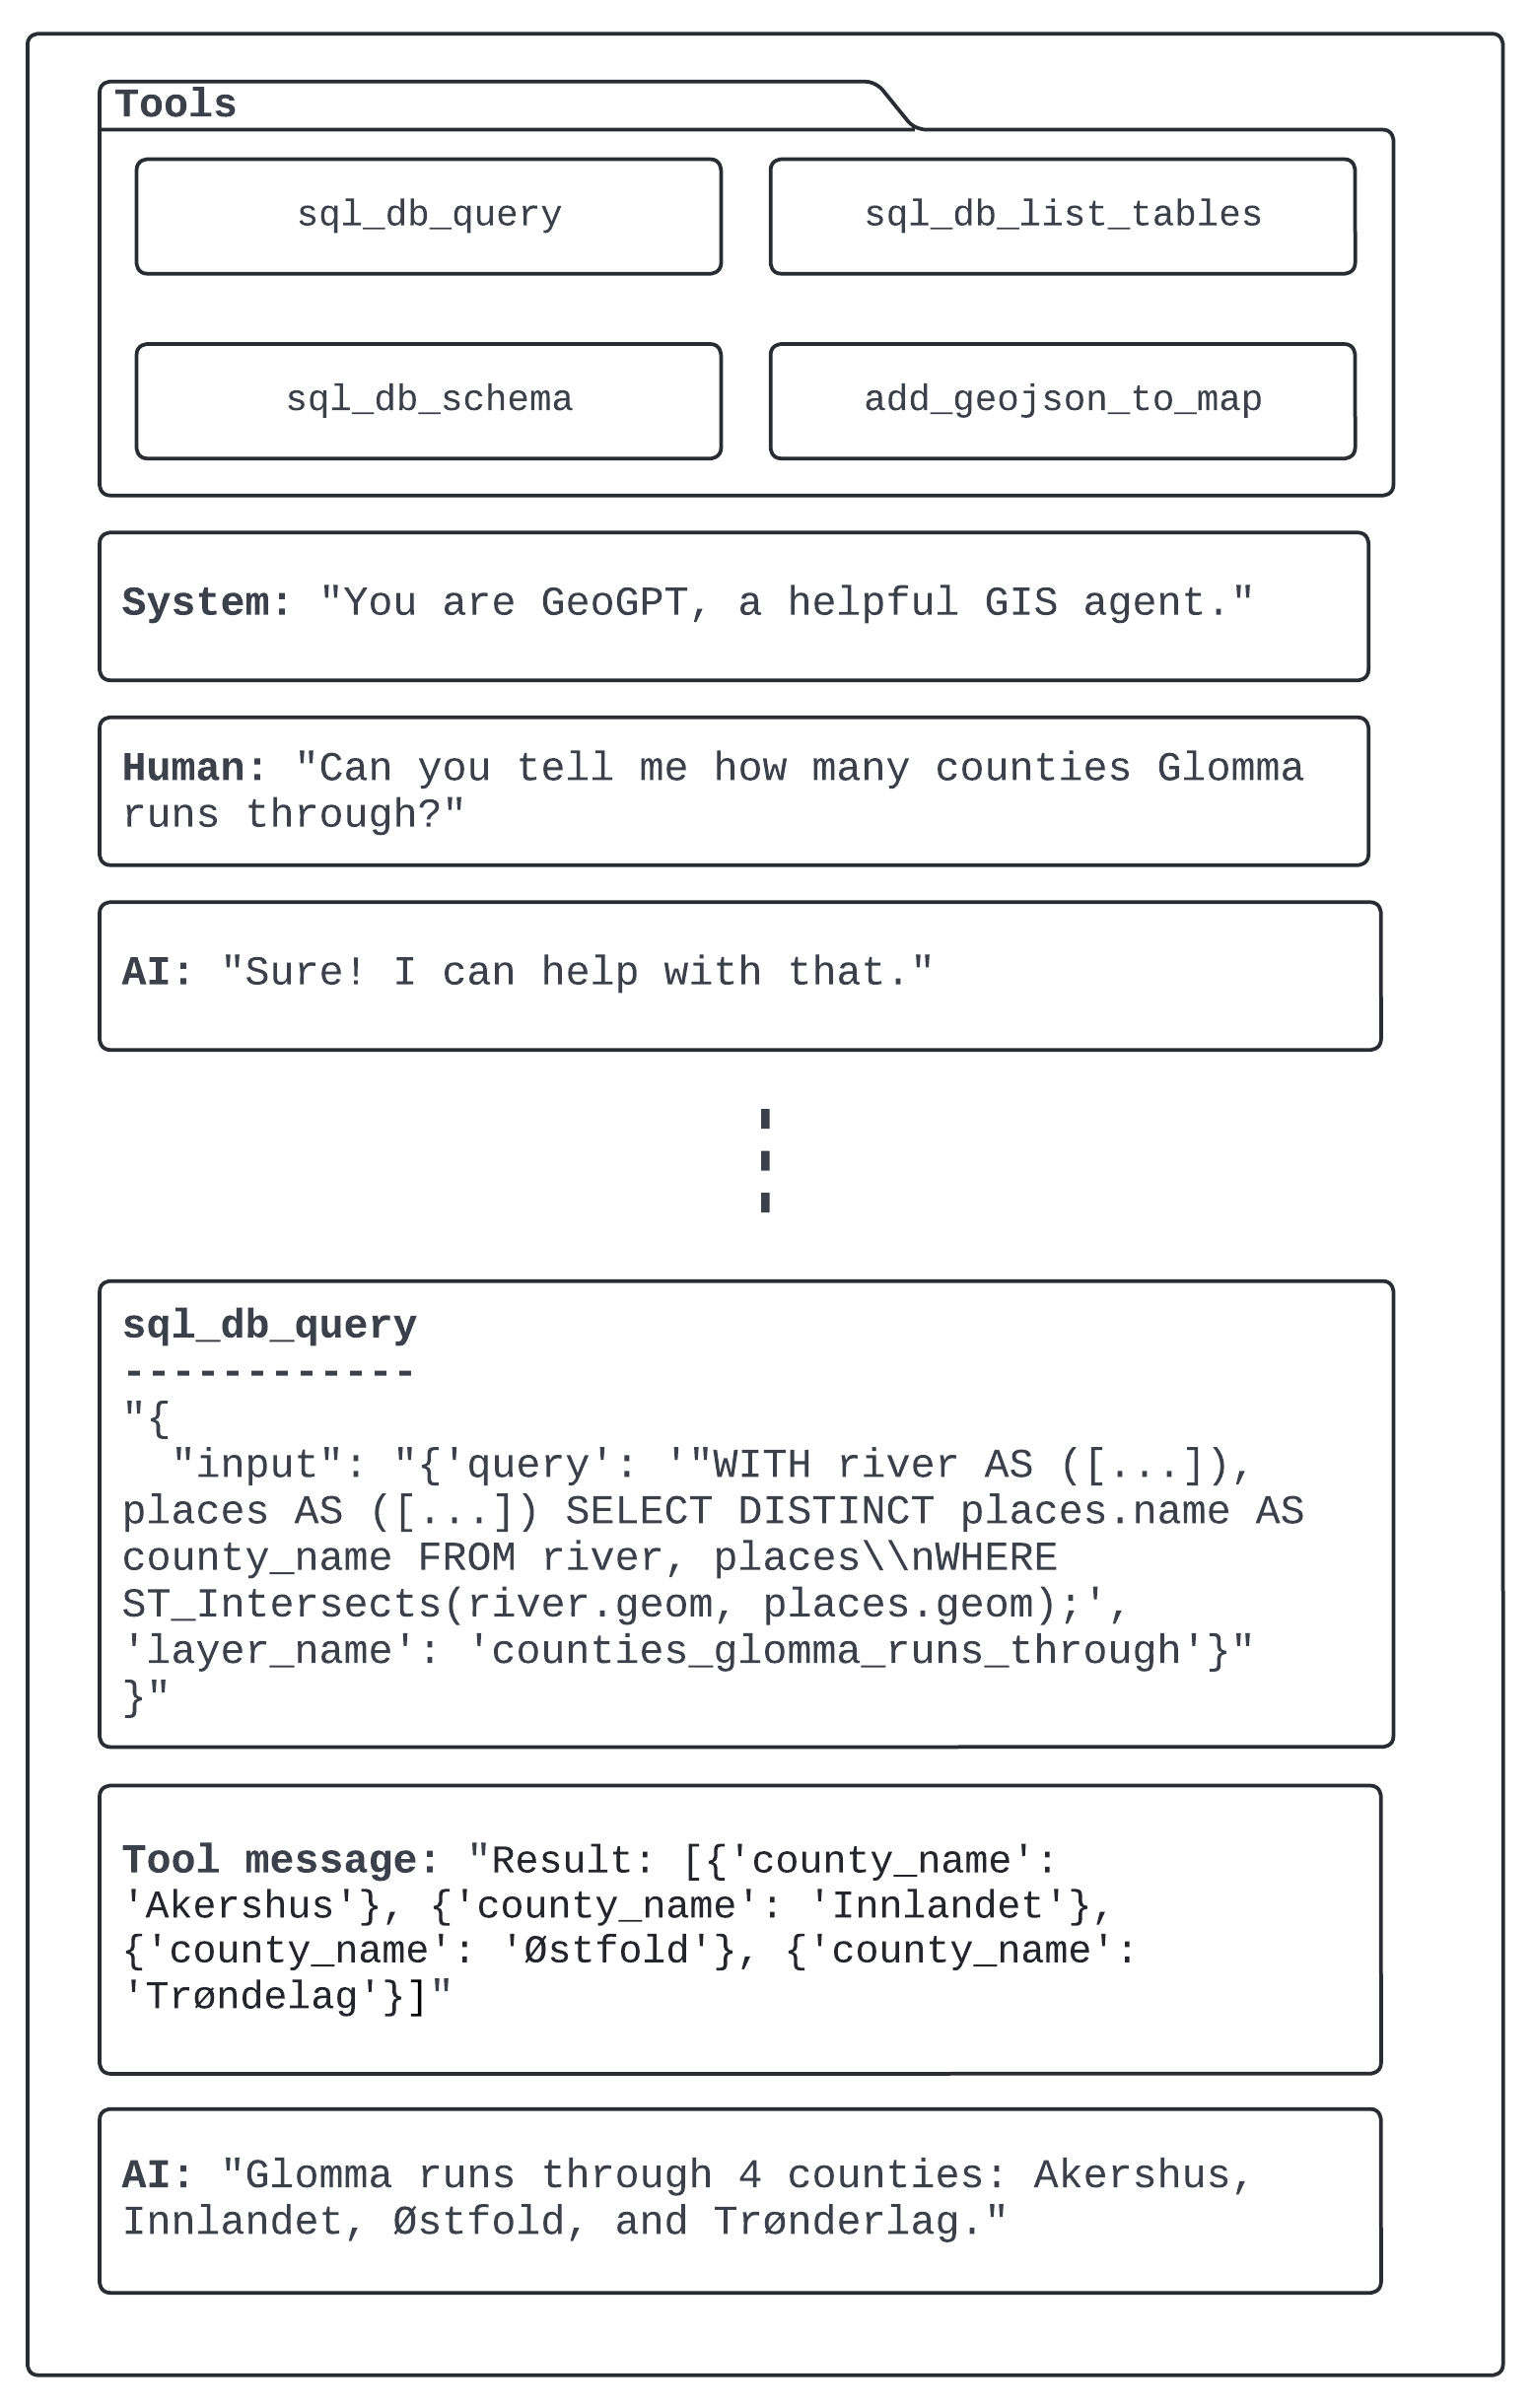
\includegraphics[width=0.9\textwidth]{chat_diagram.png}
    \caption{Example of a chat trace}
    \label{fig:chat-trace-example}
\end{figure}

\subsection{Tools}
\label{subsec:tools}

\autoref{tbl:agent-tool-overview} shows an overview of the tools that are available to each of the agents. As described in \autoref{subsec:function-calling}, these are defined by a name, an overall description of the tool's functionality, and a description of the parameters the tool expects.

The \acrshort{acr:ogc} \acrshort{acr:api} Features agent has access to a total of five tools. \textbf{\texttt{list\_collections}}, which takes no parameters, sends a \texttt{GET} request to the \texttt{/collections} endpoint and uses the response to construct a string listing the names of available collections along with their descriptions. The tool is designed to give the agent an overview of what kinds of data are available. Using the response from \texttt{list\_collections} the agent can now invoke the \textbf{\texttt{get\_collections\_info}}. This tool takes a list of collection names and returns relevant information for each of these collections. This includes the \acrshort{acr:json} response from the \enquote{landing page} of the collection, presenting details such as the collection description, spatial extent, and available attributes. In addition to this information, there is a list of common values for certain high-cardinality attributes, along with the prevalence of each value in percentages. \autoref{code:attribute-prevalences} shows an example of this. This is achieved by querying a large number of features from \texttt{/collections/\{collection\_id\}} and calculating the prevalences between them.

\begin{lstlisting}[
    caption=Prevalences of common values for the \textit{fclass} attribute in the \textit{osm\_natural\_points} collection,
    label=code:attribute-prevalences
]
Property: fclass
    tree: 71.1%
    peak: 27.2%
    beach: 0.9%
    cave_entrance: 0.5%
    spring: 0.2%
    cliff: 0.1%
    volcano: 0.0%
\end{lstlisting}

The \textbf{\texttt{query\_collection}} tool is used to retrieve features from a collection. It takes a collection name, a \acrshort{acr:cql} filter, a bounding box, and a layer name. The \acrshort{acr:cql} filter and bounding box allow for retrieval of a subset of the features of the collection being queried. Based on the parameters an URL like this is constructed:

\begin{quote}
    https://localhost:9001/collections/\{collection\_id\}/items.json?limit=10000\&filter=\{cql\_filter\}\&\{bbox\}
\end{quote}

The features retrieved from this query is saved on the working directory on the LangChain server as \enquote{\{layer\_name\}.geojson}, as a side effect of the tool. The message returned from the tool reads something like this: \enquote{Query returned 5627 features.} If the GeoJSON itself were returned as a tool message, this would quickly bloat the context window of the \acrshort{acr:llm}, and therefore it is avoided.

\begin{table}[h]
    \centering
    \caption{Overview of each agent's tools}
    \label{tbl:agent-tool-overview}
    \begin{tabularx}{0.7\textwidth}{XX}
        \toprule
        \textbf{Agent Type}                            & \textbf{Tools}                  \\
        \midrule
        \acrshort{acr:ogc} \acrshort{acr:api} Features & \texttt{list\_collections}      \\
                                                       & \texttt{get\_collections\_info} \\
                                                       & \texttt{query\_collection}      \\
                                                       & \texttt{python\_repl\_ast}      \\
                                                       & \texttt{add\_geojson\_to\_map}  \\
        \midrule
        Python                                         & \texttt{python\_repl\_ast}      \\
                                                       & \texttt{add\_geojson\_to\_map}  \\
        \midrule
        \acrshort{acr:sql}                             & \texttt{sql\_db\_list\_tables}  \\
                                                       & \texttt{sql\_db\_schema}        \\
                                                       & \texttt{sql\_db\_query}         \\
                                                       & \texttt{add\_geojson\_to\_map}  \\
        \bottomrule
    \end{tabularx}
\end{table}

Common for both the \acrshort{acr:ogc} \acrshort{acr:api} Features agent and the Python agent is the \textbf{\texttt{python\_repl\_ast}} tool. This tool accepts a string of Python code, executes said Python code, and returns whatever the code prints to the standard output in a so-called \acrfull{acr:repl}. In case the code errors, the error message is returned instead. This Python tool is the main way for these two agents perform geospatial analyses. An advantage of using \acrshortpl{acr:repl} is that the code can be executed in blocks, with variables from one block being shared with other blocks. This means that the first block may load large files into memory --- an often time-consuming operation --- while subsequent blocks can reuse this in-memory variable, even if that block should error. This allows the \acrshort{acr:llm} to quickly retry whenever the code errors or if the outcome of the initial code wasn't as expected. The \acrshort{acr:ogc} \acrshort{acr:api} Features agent will have available the files it downloaded using the \texttt{query\_collection} tool for analysis using Python, whereas the Python agent will have files corresponding to all collections available for analysis. These files are stored locally on the machine and they are added to the agent's working directory at system launch using symbolic links\footnote{\url{https://en.wikipedia.org/wiki/Symbolic_link}}. This is because a new working directory is created every time a new agent is created in order to give each agent a \enquote{clean canvas} to work from.

\textbf{\texttt{add\_geojson\_to\_map}} is the only tool that is common for all three agent types. The tool's job is to add layers to the map on the client. It takes two parameters: the name/path of a GeoJSON file stored on the LangChain server's working directory and a layer name. Invoking the tool will send a message to the client including the full path to the file on the server. The client will then make a \texttt{GET} request to the server on the \texttt{/geojson} endpoint, asking for the contents of this file to be returned so that it can be added to the map.

The \acrshort{acr:sql} agent has tools very similar to the \acrshort{acr:ogc} \acrshort{acr:api} Features agent. The \acrshort{acr:sql} agent is connected directly to the same database that the Features \acrshort{acr:api} is served on top of. \textbf{\texttt{sql\_db\_list\_tables}} is a tool that will list all database tables along with their description. \textbf{\texttt{sql\_db\_schema}} takes a list of table names and will return information about attributes, prevalence of different values in high-cardinality columns, etc., about these tables, much like \texttt{get\_collections\_info}. \textbf{\texttt{sql\_db\_query}} takes as parameter arbitrary \acrshort{acr:sql} code executes this code against the database. The tool will make sure that any query result that has a geospatial component will be stored as GeoJSON on the server. This is required to make it possible to add the geometries to the client map.

\begin{lstlisting}[
    language=json,
    caption=Example of a tool definition,
    label=code:tool-definition-example
]
{
  "type": "function",
  "function": {
    "name": "get_collections_info",
    "description": "Get the schema and sample rows for the specified collections.",
    "parameters": {
      "type": "object",
      "properties": {
        "collection_names": {
          "description": "A list of the collection_names names for which to return the schema.",
          "type": "array",
          "items": {
            "type": "string"
          }
        }
      },
      "required": [
        "collection_names"
      ]
    }
  }
}
\end{lstlisting}




\subsection{Prompt Templating}
\label{subsec:prompt-templating}






\glsresetall



\chapter{Experiments}
\label{cha:experiments}

\Autosectionref{sec:experimental-setup} of the \nameref{cha:experiments} chapter will describe the methodology and rationale behind the two experiments conducted in this thesis. The first experiment, presented in \autoref{subsec:benchmarking-setup}, assesses GeoGPT's ability to solve common \acrshort{acr:gis} tasks through a new \acrshort{acr:gis} benchmarking dataset. The other experiment, presented in \autoref{subsec:prompt-quality-test-setup}, will assess the importance of the quality of the prompt passed from the user to GeoGPT. \Autosectionref{sec:datasets} lists the datasets used in the experiments. \Autosectionref{sec:experimental-results} presents the experimental results and offers interpretations of the findings from the experiments. It will also present several example results, including screenshots of the application and code that generated by GeoGPT.

\section{Experimental Setup}
\label{sec:experimental-setup}

\begin{comment}
Trying and failing is a major part of research. However, to have a chance of success you need a plan driving the experimental research, just as you need a plan for your literature search. Further, plans are made to be revised and this revision ensures that any further decisions made are in line with the work already completed.

The plan should include what experiments or series of experiments are planned and what questions the individual or set of experiments aim to answer. Such questions should be connected to your research questions, so that in the evaluation of your results you can discuss the results wrt to the research questions.
\end{comment}

\begin{comment}
The experimental setup should include all data --- parameters, etc. --- that would allow a person to repeat your experiments.
This will thus be the actual instantiation for each experiment of the general architecture described in Chapter~\ref{cha:architecture}.
\end{comment}

% The experiments conducted using the above-mentioned \acrshort{acr:gis} benchmark are divided into two approaches. The first approach, presented in \autoref{subsec:benchmarking-setup}, is intended to evaluate GeoGPT's ability to solve a variety of geospatial tasks. The second approach, presented in \autoref{subsec:prompt-quality-test-setup}, aims to uncover the importance of the quality of the initial user prompt. \Autosubsectionref{subsec:hardware-and-model-version} describes the hardware on which the experiments were executed, and the specific \acrshortpl{acr:llm} that were used.

This section will explain the concept and setup of the two experiments mentioned in the paragraph above. \Autosectionref{subsec:benchmarking-setup} will describe the setup for the \acrshort{acr:gis} benchmark experiments, while \autoref{subsec:prompt-quality-test-setup} will explain the setup for the prompt quality experiment. \Autosubsectionref{subsec:hardware-and-model-version} describes the hardware on which the experiments were conducted, and the specific \acrshortpl{acr:llm} that were used.

\subsection[GIS Benchmark Experiment]{\acrshort{acr:gis} Benchmark Experiment}
\label{subsec:benchmarking-setup}

% In order to investigate how an \acrshort{acr:llm}-based \acrshort{acr:gis} agent most comfortably accesses geospatial data, a decision was made to include three different methods for data access in the experiments. The first method for data access is to have the files described in \autoref{sec:datasets} remain untouched. The files would be stored locally on the computer on which the experiments are conducted, and GeoGPT, which runs on the same computer, would be able to interact with the data through the code it generates. These files are made available in GeoGPT's working directory. The second method used is to load the data into a spatial \acrshort{acr:sql} database and provide the model with database schemas that can be used to generate queries. The datasets were uploaded to a Dockerized PostGIS database using QGIS's DB Manager plugin. The third method for data access is to use the \acrshort{acr:ogc} \acrshort{acr:api} Features standard. This method exposes the data stored in the PostGIS database through a web \acrshort{acr:api} that allows consumers of the \acrshort{acr:api} to download the data over \acrshort{acr:http} as GeoJSON.

The first experiment will measure the abilities of GeoGPT three agent types to produce correct answers. It will also measure cost and time taken to generate answers, and the agent's ability to produce similar answers consistently (repeatability). To do this, a benchmarking dataset was constructed. This is a set of 12 GIS-related questions with corresponding correct answers, and can be viewed in its entirety in \autoref{tbl:questions-quantitative}. The \acrshort{acr:gis} benchmark experiment will seek to compare the performance of GeoGPT's three agents. Each of the 12 questions will be asked three times per agent type. Thus, the total number of test runs becomes the following:

$$12 \text{ questions} \cdot 3 \text{ agent types} \cdot 3 \text{ repetitions} = 108 \text{ tests}$$

The following sections, named \enquote{\nameref{subsubsec:outcome-evaluation}}, \enquote{\nameref{subsubsec:cost-and-duration}}, \enquote{\nameref{subsubsec:repeatability}}, will go into detail on the different ways that the results are evaluated.

\subsubsection{Outcome Evaluation}
\label{subsubsec:outcome-evaluation}

Each of the 108 GeoGPT-generated answers will be manually evaluated based on how well the question was answered, and this outcome will be annotated as one of the following: \textit{success}, \textit{partial success}, and \textit{failure}. \autoref{tbl:test-outcome-enum} shows the guidelines used when assigning outcome scores.

\begin{table}[htbp]
    \centering
    \caption[Guidelines for evaluating outcome of tests]{Guidelines for evaluating outcome of tests}
    \label{tbl:test-outcome-enum}
    \begin{tabularx}{0.9\textwidth}{p{3cm}X}
        \toprule
        \textbf{Outcome} & \textbf{Guideline}                                                                                                                                                                                  \\
        \midrule
        Success          & The question was answered correctly and little to no follow-up from the user was required to produce the desired outcome. No false assumptions were made by the system when answering the question. \\
        Partial Success  & Portions of the question were answered correctly or semi-correctly, and/or some follow-up from the user was required to guide the system toward the solution.                                       \\
        Failure          & The question was answered incorrectly, and/or false assumptions were made by the system while attempting to answer the question.                                                                    \\
        \bottomrule
    \end{tabularx}
\end{table}


\subsubsection{Cost and Duration}
\label{subsubsec:cost-and-duration}

The application is hooked up to LangChain AI's tracing system, \textit{LangSmith}.\footnote{\url{https://www.langchain.com/langsmith} (last visited on 2nd June 2024)} Apart from being a useful tool for debugging purposes, it provides a simple way to obtain detailed data on token and time usage for a particular run, as well as the total cost of the run, in American dollars. Further details, and screenshots of LangSmith's interface, can be found in \autoref{app:langsmith}.

Box plots will be used to compare these three metrics for the different agents. The box plots follow the description for box plots found on Wikipedia.\footnote{\url{https://matplotlib.org/stable/api/_as_gen/matplotlib.pyplot.boxplot.html} (last visited on 2nd June 2024)}\footnote{\url{https://en.wikipedia.org/wiki/Box_plot} (last visited on 2nd June 2024)} Box plots allow us to easily see where the 0th ($Q_0$), 25th ($Q_1$), 50th ($Q_2$), 75th ($Q_3$), and 100th ($Q_4$) percentiles of the datasets lie, as well as the dataset's outliers. Outliers are those data points that fall more than 50\% outside the interquartile range, which is the distance between $Q_3$ and $Q_1$ in each direction.

\subsubsection{Repeatability}
\label{subsubsec:repeatability}

Another aspect that the \acrshort{acr:gis} benchmark experiment will try to evaluate, is the consistency of the system --- its ability to produce similar responses, repeatedly. The outcomes scores are encoded using the ordinal encoding presented \autoref{tbl:outcome-encoding}. A higher value indicates a better outcome. Standard deviations are calculated for each triplet of identical test samples (samples where the question and the agent type remained the same), using these encoded outcomes. This will serve as a suitable measure for assessing repeatability.

\begin{table}[htbp]
    \centering
    \caption{Ordinal encodings for outcome scores}
    \label{tbl:outcome-encoding}
    \begin{tabularx}{0.5\textwidth}{XX}
        \toprule
        \textbf{Outcome} & \textbf{Encoded Value} \\
        \midrule
        Success          & 2                      \\
        Partial Success  & 1                      \\
        Failure          & 0                      \\
        \bottomrule
    \end{tabularx}
\end{table}


\subsection{Prompt Quality Experiment}
\label{subsec:prompt-quality-test-setup}

A second experiment is constructed to evaluate the importance of the initial question/prompt from the user. As stated in the \nameref{sec:background-and-motivation} chapter, part of the motivation for developing an \acrshort{acr:llm}-based \acrshort{acr:gis} like GeoGPT is to make \acrshort{acr:gis} more accessible to non-experts. It is therefore interesting to assess the extent to which a carefully constructed prompt by a \acrshort{acr:gis} expert can enhance the system's output.

For these experiments, the three hardest questions from the \acrshort{acr:gis} benchmark experiment were picked. Then, for each of these three questions, a \textit{novice}-level and an \textit{expert}-level prompt was constructed. The novice-level prompt is as simple as possible, while the expert-level prompt is more elaborate and written as a step-by-step recipe for solving the problem. Despite their differences, the prompts should ideally produce the same answer.

\subsection[Hardware and LLM Version]{Hardware and \acrshort{acr:llm} Version}
\label{subsec:hardware-and-model-version}

All experiments were conducted on a Lenovo ThinkPad E490, which has an Intel{\textregistered} Core\texttrademark{} i7-8565U CPU @ 1.80GHz processor, 15.8 GB usable \acrshort{acr:ram}, and 256 GB \acrshort{acr:ssd} storage. Everything but the \acrshort{acr:llm} inference was done locally. \acrshort{acr:llm} inference (text generation) was done using OpenAI's Inference \acrshort{acr:api}.

It is worth noting that two slightly different models were used during testing. This is due the release of the \texttt{gpt-4-turbo-2024-04-09} model in mid-April. According to OpenAI, \enquote{this new model is better at math, logical reasoning, and coding} compared to \texttt{gpt-4-0125-preview},\footnote{OpenAI has a GitHub repository containing the code they use to evaluate their \glspl{acr:llm} and benchmark results for OpenAI models and reference models from other companies: \url{https://github.com/openai/simple-evals} (last visited on 2nd June 2024)} which is the model that was used for the first test runs. At \texttt{gpt-4-turbo-2024-04-09}'s release, a decision was made to use this for the remaining experiments. The experiments that had already been conducted were not re-run due to time constraints and a confidence that these slight model upgrades would not significantly change the outcome of the experiments.


\section{Datasets}
\label{sec:datasets}

A total of eighteen datasets were used in the experiments, all downloaded from a website called \enquote{Geofabrik}.\footnote{\url{https://download.geofabrik.de/europe/norway.html} (last visited on 2nd June 2024)} \textit{Geofabrik}, which is German for \enquote{geo factory}, is a company that \enquote{extract, select, and process free geodata}. They have gathered data from OpenStreetMap and published them as a collection of shapefiles, dividing them into categories such as \enquote{places of worship}, \enquote{points of interest}, and \enquote{traffic}. Data can be downloaded for different regions of the world, but for the experiments conducted in this thesis, only data for Norway was used. \autoref{tbl:datasets} lists the datasets, along with short descriptions of their contents, and the number of features for each dataset. Common for all datasets is their \emph{fclass} attribute, which is short for \emph{feature class}. Some datasets have additional attributes, such as the \emph{maxspeed} attribute in the road dataset and the \emph{type} attribute in the building dataset. \autoref{fig:datasets-trondheim} shows a plot containing four selected datasets, constrained to a bounding box of Trondheim. This plot was created by GeoGPT.

\begin{longtable}{p{3cm}p{2cm}p{5.7cm}p{2.5cm}}
    \caption{Datasets used in the experiments}                                                                                                                                                                                                              \\
    \label{tbl:datasets}                                                                                                                                                                                                                                    \\
    \toprule
    \textbf{Dataset}   & \textbf{Type} & \textbf{Description}                                                                                                                                                                         & \textbf{\#Features} \\
    \midrule
    \endfirsthead

    \multicolumn{4}{c}{{\bfseries Table \thetable\ continued from previous page}}                                                                                                                                                                           \\
    \toprule
    \textbf{Dataset}   & \textbf{Type} & \textbf{Description}                                                                                                                                                                         & \textbf{\#Features} \\
    \midrule
    \endhead

    \midrule
    \multicolumn{4}{r}{Continued on next page}                                                                                                                                                                                                              \\
    \midrule
    \endfoot

    \bottomrule
    \endlastfoot

    Buildings          & Polygon       & Contains building outlines. Its \emph{type} attribute can have values like \enquote{house}, \enquote{university}, and \enquote{restaurant}.                                                  & 4,147,645           \\
    Land Use           & Polygon       & Represents areas designated to different purposes and activities. Its \emph{fclass} attribute can have values like \enquote{forest}, \enquote{farmland}, and \enquote{residential}.          & 541,452             \\
    Natural            & Point         & Contains outlines of various objects found in nature. Its \emph{fclass} attribute can have values like \enquote{beach}, \enquote{glacier}, and \enquote{cave\_entrance}.                     & 119,725             \\
    Natural            & Polygon       & Similar to the point data equivalent.                                                                                                                                                        & 6,665               \\
    Places of Worship  & Point         & Common values for \emph{fclass} attribute: \enquote{christian}, \enquote{buddhist}, and \enquote{muslim}.                                                                                    & 311                 \\
    Places of Worship  & Polygon       & Similar to the point data equivalent.                                                                                                                                                        & 2,520               \\
    Places             & Point         & Common values for \emph{fclass} attribute: \enquote{farm}, \enquote{village}, and \enquote{island}.                                                                                          & 178,997             \\
    Places             & Polygon       & Similar to the point data equivalent.                                                                                                                                                        & 5,689               \\
    Points of Interest & Point         & Common values for \emph{fclass} attribute: \enquote{tourist\_info}, \enquote{bench}, and \enquote{kindergarten}.                                                                             & 117,677             \\
    Points of Interest & Polygon       & Similar to the point data equivalent.                                                                                                                                                        & 45,825              \\
    Railways           & Line          & Common values for \emph{fclass} attribute: \enquote{rail}, \enquote{subway}, and \enquote{tram}. Also has True/False attributes \emph{bridge} and \emph{tunnel}.                             & 14,008              \\
    Roads              & Line          & Common values for \emph{fclass} attribute: \enquote{rail}, \enquote{subway}, and \enquote{tram}. Has additional attributes \emph{oneway}, \emph{maxspeed}, \emph{bridge}, and \emph{tunnel}. & 1,741,929           \\
    Traffic            & Point         & Common values for \emph{fclass} attribute: \enquote{crossing}, \enquote{street\_lamp}, and \enquote{parking}.                                                                                & 98,860              \\
    Traffic            & Polygon       & Common values for \emph{fclass} attribute: \enquote{parking}, \enquote{pier}, and \enquote{dam}.                                                                                             & 45,623              \\
    Transport          & Point         & Common values for \emph{fclass} attribute: \enquote{bus\_stop}, \enquote{ferry\_terminal}, and \enquote{railway\_station}.                                                                   & 91,627              \\
    Transport          & Polygon       & Similar to the point data equivalent.                                                                                                                                                        & 935                 \\
    Water              & Polygon       & Common values for \emph{fclass} attribute: \enquote{water}, \enquote{wetland}, and \enquote{river\_bank}.                                                                                    & 1,861,199           \\
    Waterways          & Line          & Common values for \emph{fclass} attribute: \enquote{stream}, \enquote{river}, and \enquote{canal}.                                                                                           & 833,253             \\
\end{longtable}


\begin{figure}
    \centering
    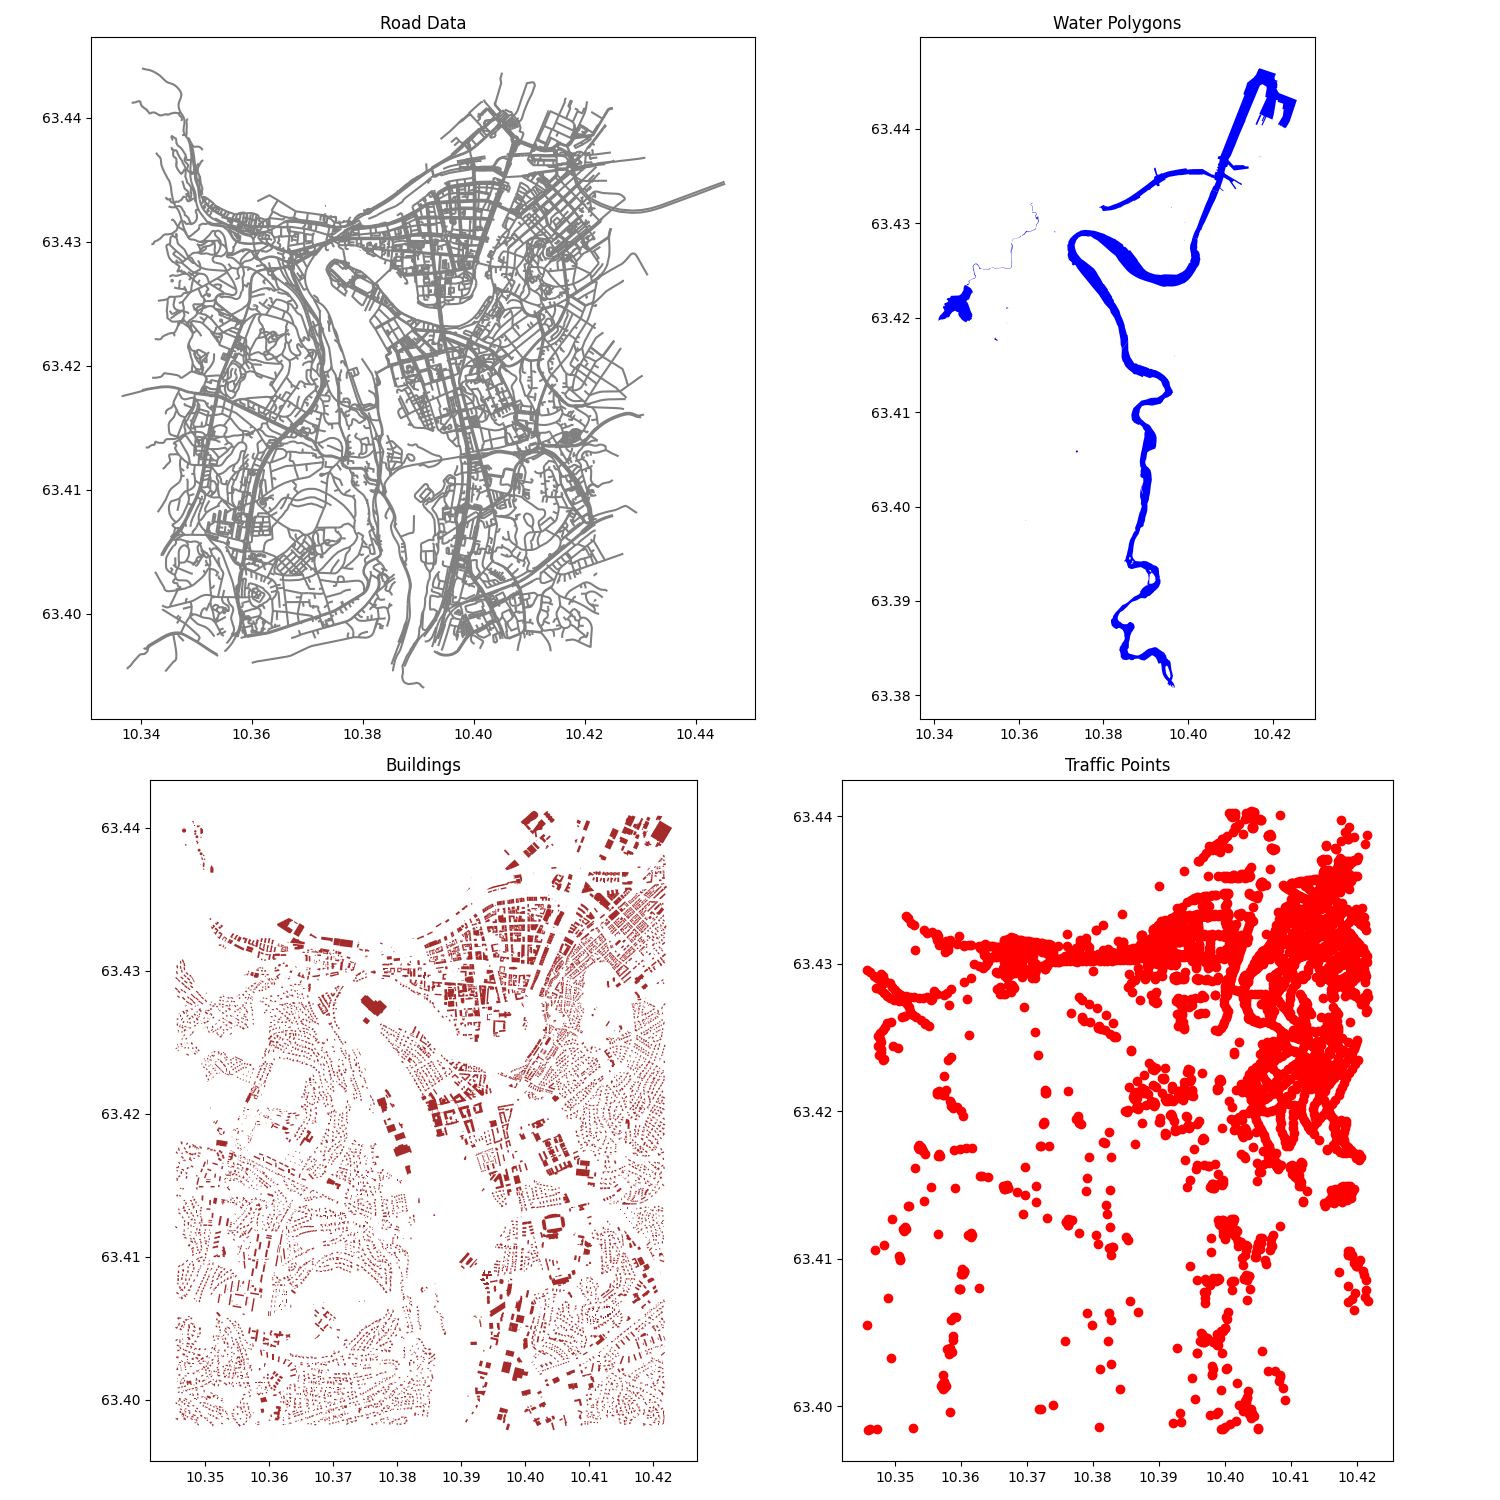
\includegraphics[width=\textwidth]{trondheim_datasets.png}
    \caption[A plot of four selected datasets constrained to a polygon of Trondheim]{A plot of four selected datasets constrained to a polygon of Trondheim. From top-left, clockwise: road lines, water polygons, traffic points, and building polygons. These plots were generated by GeoGPT.}
    \label{fig:datasets-trondheim}
\end{figure}

\FloatBarrier


\section{Experimental Results}
\label{sec:experimental-results}

\begin{comment}
Results should be clearly displayed and should provide a suitable representation of your results for the points you wish to make.
Graphs should be labelled in a legible font. If more than one result is displayed in the same graph, then these should be clearly marked.
Please choose carefully rather than presenting every result. Too much information is hard to read and often hides the key information you wish to present. Make use of statistical methods when presenting results, where possible to strengthen the results.
Further, the format of the presentation of results should be chosen based on what issues in the results you wish to highlight.
You may wish to present a subset in the experimental section and provide additional results in an appendix.
Point out specifics here but save the overall/general discussion to the Discussion chapter.
\end{comment}

\Autosubsectionref{subsec:quantitative-results} and \autoref{subsec:prompt-quality-test-results} will present the outcome of the experiments presented in \autoref{subsec:benchmarking-setup} and \autoref{subsec:prompt-quality-test-setup}, respectively. Visualizations for this section were created using Matplotlib,\footnote{\url{https://matplotlib.org/} (last visited on 2nd June 2024)} a Python library suitable for creating bar charts, box plots, etc.


\subsection[GIS Benchmark Experiment --- Results]{\acrshort{acr:gis} Benchmark --- Results}
\label{subsec:quantitative-results}

\subsubsection{Outcome Evaluation}

\autoref{fig:outcome-distribution} shows a bar charts for the outcome distribution between GeoGPT's three agents. The \acrshort{acr:ogc} \acrshort{acr:api} Features agent and the Python agent have comparable results, whereas the \acrshort{acr:sql} agent performs significantly better than the other two. The \acrshort{acr:sql} agent has a success rate of 69.4\%, while the other two share a success rate of 38.9\%. Possible reasons for this are discussed in \autoref{sec:why-sql-better} of the \nameref{cha:discussion}.

\begin{figure}[htbp]
    \centering
    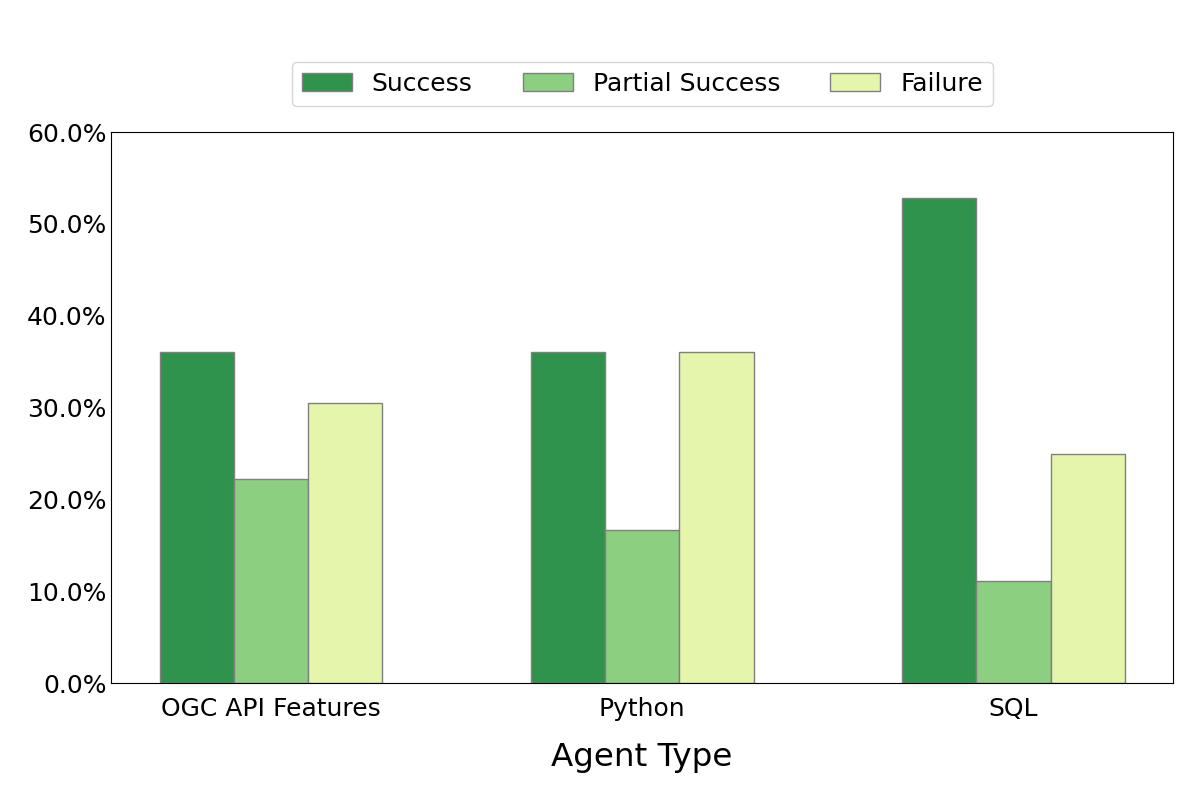
\includegraphics[width=\textwidth]{outcome_distribution_bar_chart.png}
    \caption[Outcome distribution between GeoGPT's different agent types]{Outcome distribution between GeoGPT's different agent types. The \acrshort{acr:ogc} \acrshort{acr:api} Features and Python agents perform similarly, while the \acrshort{acr:sql} agent outperforms them by a significant margin.}
    \label{fig:outcome-distribution}
\end{figure}

\subsubsection{Cost and Duration}

\autoref{fig:duration-box-plot} displays a box plot with a logarithmic y-axis that shows task durations between the different agent types. Here we can see that the \acrshort{acr:sql} agent spends the least amount of time per task. The \acrshort{acr:ogc} \acrshort{acr:api} Features agent has a slightly higher median, but with a few time-consuming outliers. The Python agent is the odd one out with a median of $\sim 82$ seconds, a $Q3 \sim 293$ seconds, and a $Q4 \sim 984$ seconds. The large gap from the Python agent to the other two agents it largely due to the Python agent's tendency to load large datasets into memory. For instance, when attempting the task of calculating the difference between the polygon outlining Oslo and water polygons (see \autoref{tbl:questions-quantitative} for the task formulation), the Python agent used nearly 40 minutes on the entire task. $94\%$ of the time was spent executing the code in \autoref{code:python-oslo-water-diff}. The main reason for the long execution time is line 8, where the whole \texttt{osm\_landuse\_polygons.shp} dataset is loaded into memory. This dataset has a size of $\sim 1.4 \text{ GB}$ and a total of 1,861,199 polygon features, and loading such amounts of data in this way is very time-consuming. The Python agent was the only agent with such issues because the \acrshort{acr:ogc} \acrshort{acr:api} Features agent is limited to 10,000 features per request, and the \acrshort{acr:sql} agent does not load the data into memory like the other agents do.

\begin{figure}[htbp]
    \centering
    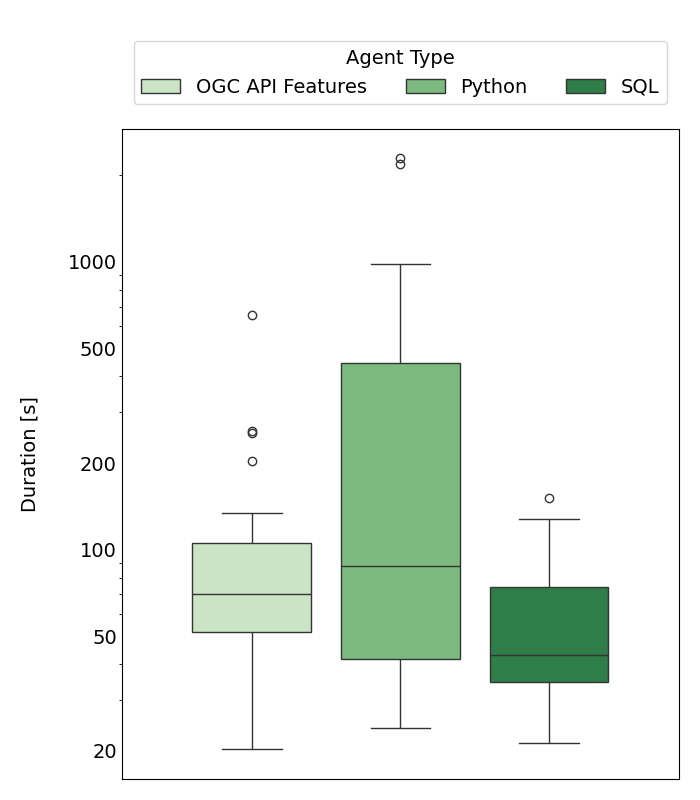
\includegraphics[width=0.6\textwidth]{duration_box_plot.png}
    \caption[Box plots comparing the time taken to generate answers between GeoGPT's agent types]{Box plots comparing the time taken to generate answers between GeoGPT's agent types. Again, the \acrshort{acr:sql} agent performs best, while the Python agent is the odd one out with very slow times compared to the other two.}
    \label{fig:duration-box-plot}
\end{figure}

\FloatBarrier

\begin{lstlisting}[
    language=Python,
    caption={[GeoGPT-generated Python code aimed at computing the difference between the outline of Oslo and residental features within it]GeoGPT-generated Python code aimed at computing the difference between the outline of Oslo, the Norwegian capital, and residental features within it. The execution time of this code block was $\sim 36$ minutes, mostly due to line 8.},
    label=code:python-oslo-water-diff,
    float
]
    import geopandas as gpd

    # Paths to the shapefiles
    landuse_path = '/tmp/tmpsutdy6it/osm_landuse_polygons.shp'
    places_path = '/tmp/tmpsutdy6it/osm_places_polygons.shp'
    
    # Load the data from shapefiles
    landuse_gdf = gpd.read_file(landuse_path)
    places_gdf = gpd.read_file(places_path)
    
    # Filter out 'residential' areas from the landuse data
    residential_gdf = landuse_gdf[landuse_gdf['fclass'] == 'residential']
     
    # Compute the spatial difference to exclude residential areas from the places data
    oslo_outline = gpd.overlay(places_gdf, residential_gdf, how='difference')
    
    # Path for the output GeoJSON file
    output_path = '/tmp/tmpsutdy6it/oslo_outline_no_residential.geojson'
    
    # Save the resulting GeoDataFrame to a GeoJSON file
    oslo_outline.to_file(output_path, driver='GeoJSON')
    
    # Output the path to the saved file
    print(output_path)    
\end{lstlisting}

\autoref{fig:cost-and-tokens} shows box plots for token usage and cost per run. Naturally, these figures appear very similar, since prices for the input tokens and generated output tokens are fixed for the models used. According to OpenAI's webpages,\footnote{\url{https://openai.com/pricing} (last visited 2nd June 2024)} they charge $\$10$ per million input tokens and $\$30$ per million output tokens for their \acrshort{acr:gpt}-4 Turbo model. From the results of the experiments, a ratio of approximately $\text{\$}10.7$ per million tokens --- either input \textit{or} output --- was calculated, which is closest to the input token price. This shows that \textit{a lot} more input tokens were used, compared to output tokens.

\begin{figure}[htbp]
    \centering
    \begin{subfigure}[b]{0.48\textwidth}
        \centering
        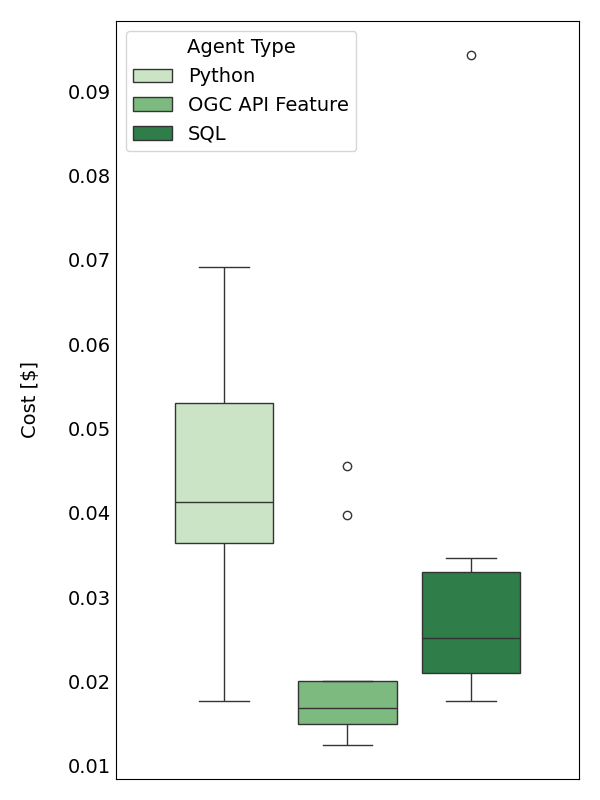
\includegraphics[width=\textwidth]{cost_box_plot.png}
        \caption{Average cost per answer between the agent types}
        \label{fig:cost-box-plot}
    \end{subfigure}
    \hfill
    \begin{subfigure}[b]{0.48\textwidth}
        \centering
        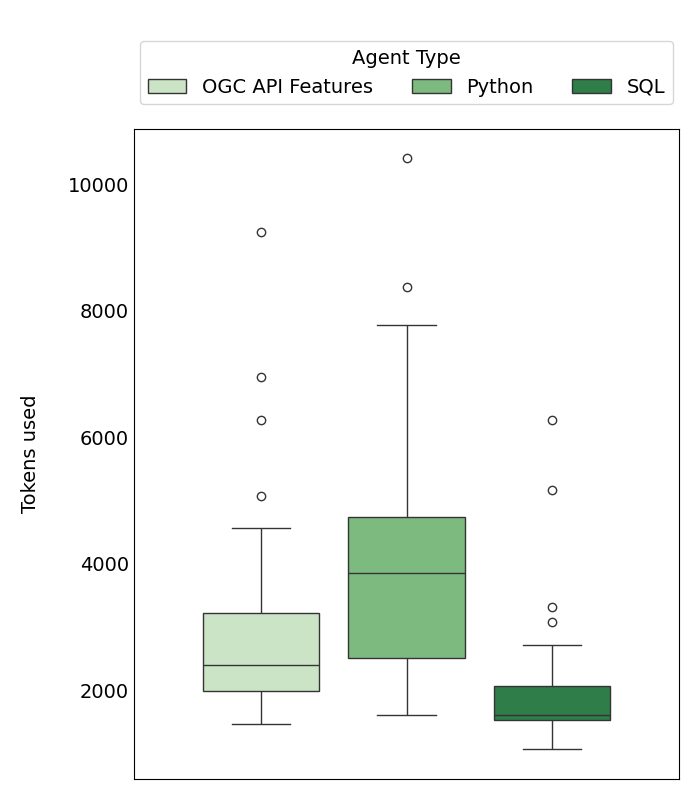
\includegraphics[width=\textwidth]{tokens_box_plot.png}
        \caption{Average token usage per answer between the agent types}
        \label{fig:tokens-box-plot}
    \end{subfigure}
    \caption[Cost and token usage between GeoGPT's different agent types]{Cost and token usage between GeoGPT's different agent types. These plots are highly correlated, but will differ somewhat because of the ratio between input and output tokens.}
    \label{fig:cost-and-tokens}
\end{figure}

An observation that can be made from the correlation matrices in \autoref{fig:correlation-matrices} is that the correlation between duration and token usage is inconsistent between the agent types. The \acrshort{acr:ogc} \acrshort{acr:api} Features agent and \acrshort{acr:sql} agent have strong correlation between these metrics, but the Python agent has next to none. This supports the observation that, for the Python agent, code execution time, particularly the time spent on expensive imports, is likely the main contributor towards the total run time.

Another observation that can be made from the \autoref{fig:correlation-matrices} is the slight negative correlation between the encoded outcome and each of the following variables: token usage, duration, and total cost. This suggests that a task that takes longer to complete, and has a higher token usage, is \textit{less} likely to produce a successful outcome. Possible reasons as to why this is the case will be explored in \autoref{subsec:dead-ends} in the \nameref{cha:discussion}.

\begin{figure}[htp]
    \centering

    \begin{subfigure}[b]{\textwidth}
        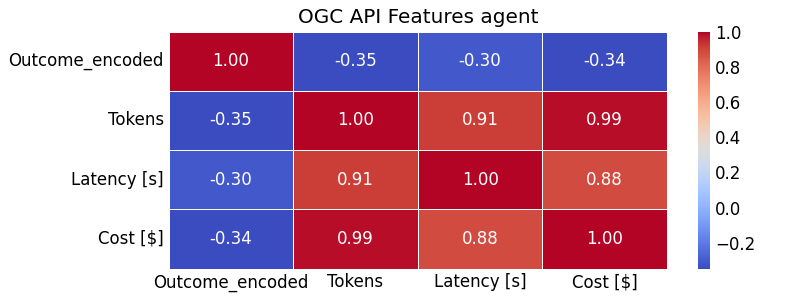
\includegraphics[width=\textwidth]{correlation_matrix_oaf.png}
        \caption{Correlation matrix for the \acrshort{acr:ogc} \acrshort{acr:api} Features agent}
        \label{fig:sub1}
    \end{subfigure}

    \vspace{1cm}

    \begin{subfigure}[b]{\textwidth}
        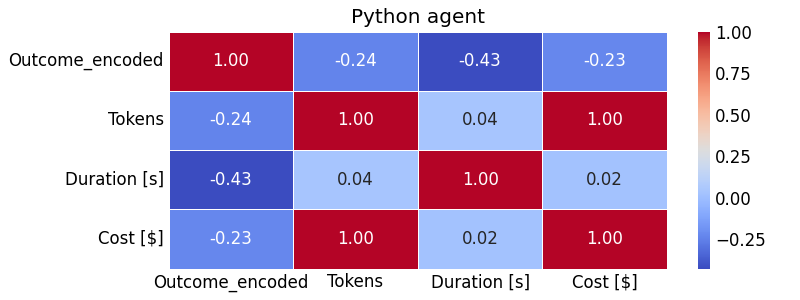
\includegraphics[width=\textwidth]{correlation_matrix_python.png}
        \caption{Correlation matrix for the Python agent}
        \label{fig:sub2}
    \end{subfigure}

    \vspace{1cm}

    \begin{subfigure}[b]{\textwidth}
        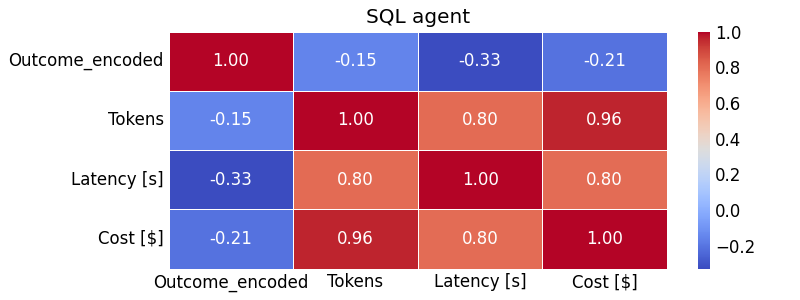
\includegraphics[width=\textwidth]{correlation_matrix_sql.png}
        \caption{Correlation matrix for the \acrshort{acr:sql} agent}
        \label{fig:sub3}
    \end{subfigure}

    \caption{Correlation matrices for the metrics recorded during the \acrshort{acr:gis} benchmark experiment for the three agent types}
    \label{fig:correlation-matrices}
\end{figure}

\subsubsection{Repeatability}

\autoref{tbl:stddev-by-agent-type} shows the average standard deviation of the outcomes for each agent type, as well as the mean of these three standard deviations. These numbers indicate that there is a notable amount of inconsistency in GeoGPT's answers when task and agent type stays the same, on average deviating with more than a third of an outcome category (0.376 for the encoded values).

\begin{table}[htbp]
    \centering
    \caption{Standard deviations of encoded outcomes for GeoGPT's agent types}
    \label{tbl:stddev-by-agent-type}
    \begin{tabularx}{0.7\textwidth}{XX}
        \toprule
        \textbf{Agent Type}                            & \textbf{Outcome Std. Deviation} \\
        \midrule
        \acrshort{acr:ogc} \acrshort{acr:api} Features & 0.552                           \\
        Python                                         & 0.337                           \\
        \acrshort{acr:sql}                             & 0.241                           \\
        \midrule
        \textbf{Mean}                                  & 0.376                           \\
        \bottomrule
    \end{tabularx}
\end{table}

\FloatBarrier

\subsubsection{Successful Responses}

% 6df94421-6c7c-470a-af8e-7013f3bc547f
\autoref{fig:glomma-counties-sql-successful} shows a successful response from GeoGPT's \acrshort{acr:sql} agent when asked how many counties the Glomma river runs through.\footnote{This run was not part of the results used for evaluation due to a bug in the \texttt{sql\_db\_query} tool that caused it to unnecessarily execute queries twice. GeoGPT's response would not be different had the bug not been present for the run, but it would have taken longer to complete.} GeoGPT correctly lists all four correct counties in a numbered list. \autoref{code:glomma-counties-sql} shows the code generated by GeoGPT for the second invocation of \texttt{sql\_db\_query}. The second invocation is nearly identical to the first one, but in the first invocation the geometry column was not included in the response, meaning GeoGPT was unable to add the results to the map. The tool informs GeoGPT about this, and the agent therefore decided to run the query again, now making sure to include the geometry column in the query result, before adding the resulting GeoJSON file to the map using the \texttt{add\_geojson\_to\_map} tool. A follow-up message instructed GeoGPT to \enquote{Add Glomma to the map}, allowing for visual verification that the answer it gave was correct.

\begin{figure}[htbp]
    \centering
    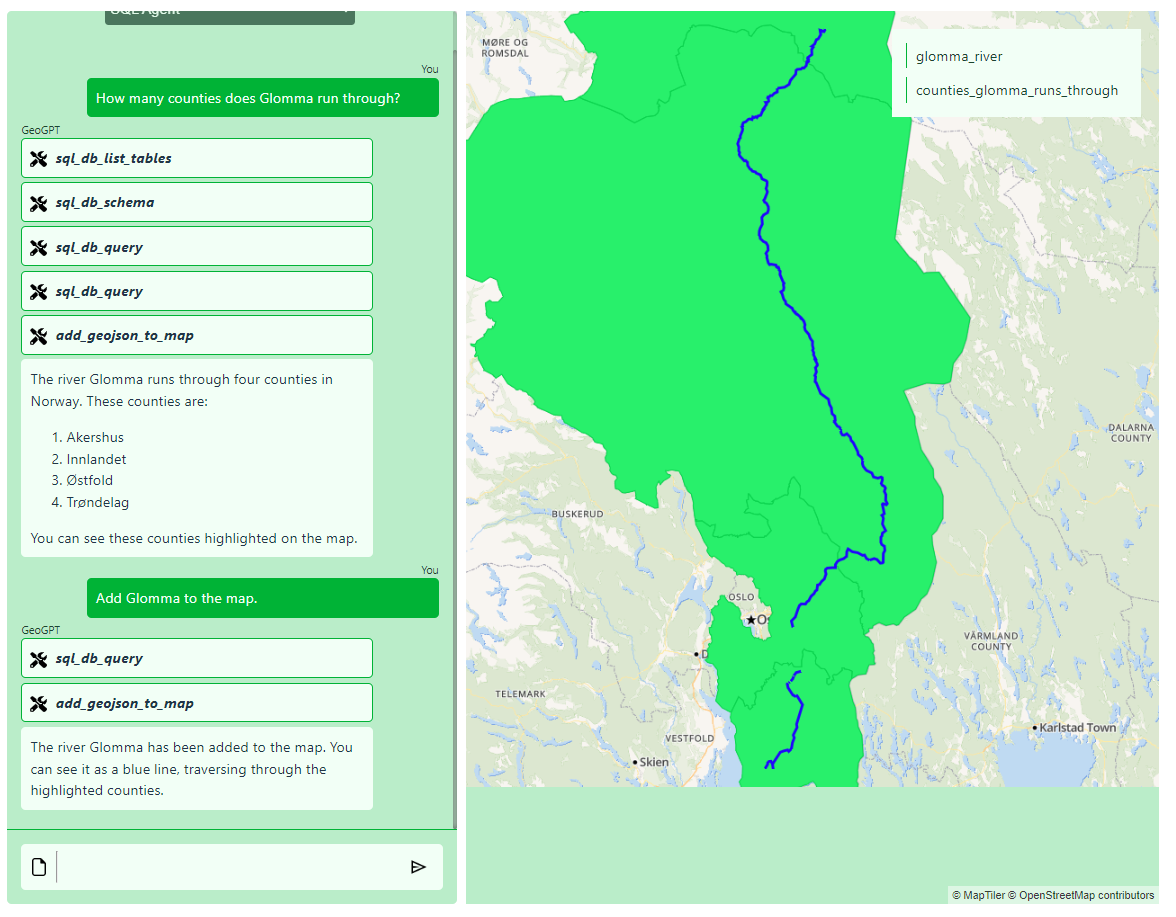
\includegraphics[width=\textwidth]{glomma_counties_sql_22.png}
    \caption[Successful response from GeoGPT's SQL agent when asked how many counties the Glomma river runs through]{Successful response from GeoGPT's \acrshort{acr:sql} agent when asked how many counties the Glomma river runs through. Using the tools available to it, GeoGPT's \acrshort{acr:sql} agent was able to to find that the river Glomma runs through the following counties: Akershus, Innlandet, Østfold, and Trøndelag. A follow-up message was added to make GeoGPT add the river geometries to the map, for verification of its results.}
    \label{fig:glomma-counties-sql-successful}
\end{figure}

\FloatBarrier

\begin{lstlisting}[
    language=sql,
    caption={[GeoGPT-generated SQL code to retrieve the counties that the Glomma river runs through]GeoGPT-generated \acrshort{acr:sql} code to retrieve the counties that the Glomma river runs through. The \texttt{ST\_Intersects} function from PostGIS was used to find the intersection between the river data and the county polygons, and the names and geometries of the counties was included in the result.},
    label=code:glomma-counties-sql,
]
WITH river AS (
    SELECT geom 
    FROM osm_waterways_lines 
    WHERE fclass = 'river' AND name ILIKE 'Glomma'
),

places AS (
    SELECT geom, name 
    FROM osm_places_polygons 
    WHERE fclass = 'county'
)

SELECT DISTINCT places.name AS county_name, places.geom AS geom
FROM river, places
WHERE ST_Intersects(river.geom, places.geom);    
\end{lstlisting}

\FloatBarrier

\autoref{fig:trees-along-munkegata-python-partial-success} shows a partially successful attempt from GeoGPT's Python agent to calculate the number of trees along Munkegata in Trondheim. While setting a definitive answer to such a question is difficult, the correct answer was set to about 100, assuming a 20-meter buffer around the line segments that make up the road. In \autoref{code:python-munkegata-bbox}, we can see how GeoGPT loads the road data around Munkegata in Trondheim, using an approximate bounding box to avoid retrieving roads named \enquote{Munkegata} in other cities. It then filters and saves the loaded data to only include features named Munkegata. In the following code block, shown in \autoref{code:python-trees-count-munkegata}, GeoGPT gets the tree data by filtering the \texttt{osm\_natural\_points} dataset on the \texttt{fclass} attribute, before loading the road data for Munkegata from \autoref{code:python-munkegata-bbox}, converting both datasets to a metric \acrshort{acr:crs}, creating a buffer around the road data, performing an intersection between the buffer, and finally printing the \texttt{tree\_count} to the standard output.

\begin{figure}[htbp]
    \centering
    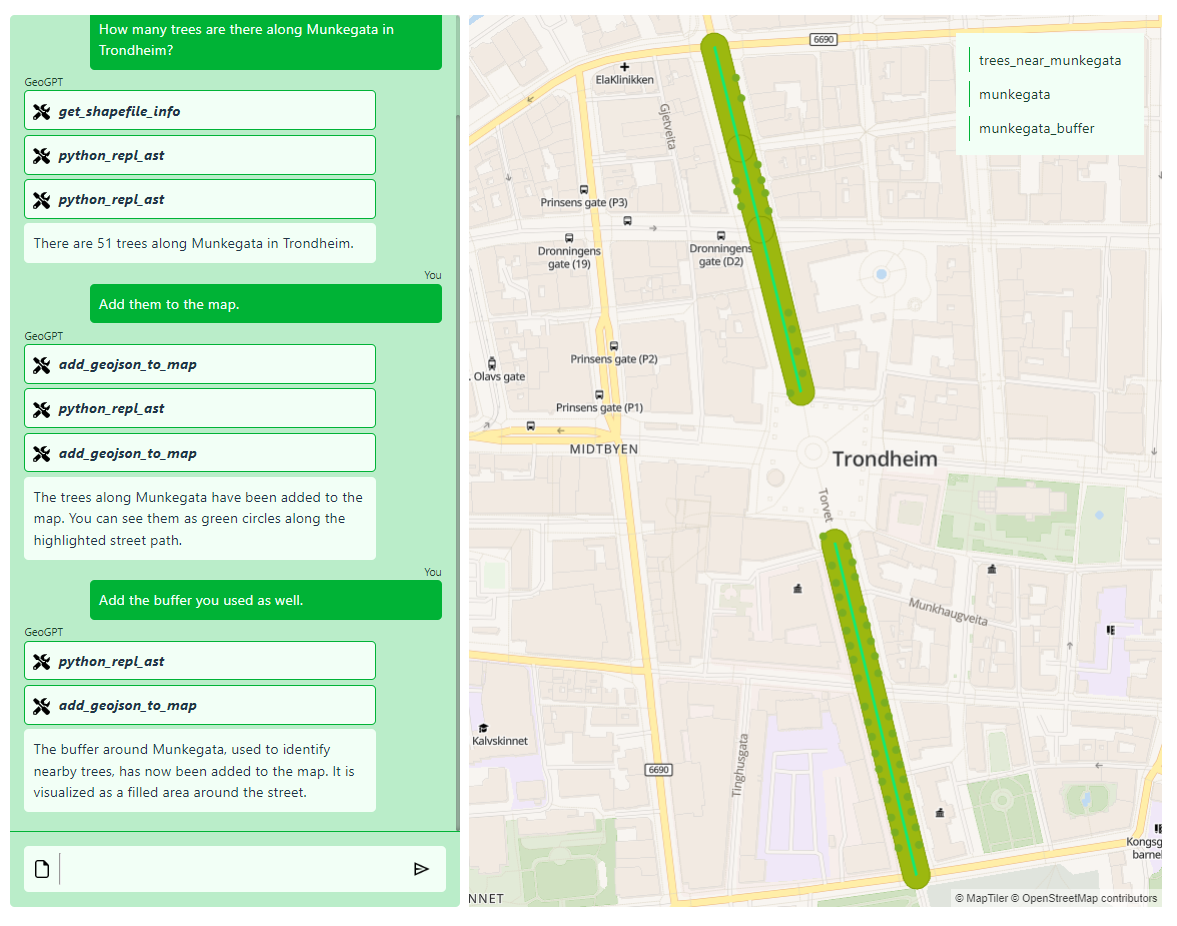
\includegraphics[width=\textwidth]{num_trees_along_munkegata_python_with_buffer.png}
    \caption[Partially successful response from GeoGPT's Python agent when asked how many trees there are along Munkegata in Trondheim]{Partially successful response from GeoGPT's Python agent when asked how many trees there are along Munkegata in Trondheim. It managed to find the road segments corresponding to Munkegata in Trondheim, but created a slightly too small buffer around it, which did not cover all the relevant trees.}
    \label{fig:trees-along-munkegata-python-partial-success}
\end{figure}

\FloatBarrier

\begin{lstlisting}[
    language=python,
    caption={[GeoGPT-generated Python code to retrieve the Munkegata road in Trondheim]GeoGPT-generated Python code to retrieve the Munkegata road in Trondheim. The bounding box, which is generated from \acrshort{acr:gpt}-4's background knowledge, covers a suitable area in the center of Trondheim, where Munkegata is located. This step is important, as a road named \enquote{Munkegata} can also be found in Oslo, which is located in a \textit{completely different} part of Norway.},
    label=code:python-munkegata-bbox,
]
import geopandas as gpd

# Load roads data with a focus on Munkegata
roads_path = '/tmp/tmpl8zsdj6m/osm_roads_lines.shp'
munkegata_bbox = (10.3910, 63.4270, 10.4030, 63.4330) # Approximate bounding box around Munkegata
munkegata_roads = gpd.read_file(roads_path, bbox=munkegata_bbox)

# Filter for Munkegata
munkegata = munkegata_roads[munkegata_roads['name'] == 'Munkegata']

# Save filtered Munkegata road to GeoJSON
munkegata_path = '/tmp/tmpl8zsdj6m/munkegata.geojson'
munkegata.to_file(munkegata_path, driver='GeoJSON')

print(munkegata_path)
\end{lstlisting}

\FloatBarrier

\begin{lstlisting}[
    language=python,
    caption={[GeoGPT-generated Python code to calculate the number of trees along Munkegata in Trondheim]Python code to calculate the number of trees along Munkegata in Trondheim. The datasets were converted to a metric \acrshort{acr:crs} (WGS 84 / UTM zone 33N), before a buffer around the road data from \autoref{code:python-munkegata-bbox} was created and used to find the intersection with the tree data. 51 trees were found, but ideally $\sim 100$ should be returned.},
    label=code:python-trees-count-munkegata,
]
from shapely.geometry import box
import geopandas as gpd

# Load the trees points
natural_points_path = '/tmp/tmpl8zsdj6m/osm_natural_points.shp'
trees = gpd.read_file(natural_points_path)

# Filter for trees
trees = trees[trees['fclass'] == 'tree']

# Load Munkegata road
munkegata_path = '/tmp/tmpl8zsdj6m/munkegata.geojson'
munkegata_road = gpd.read_file(munkegata_path)

# Project to UTM for accurate distance measurement
munkegata_utm = munkegata_road.to_crs(epsg=32633)
trees_utm = trees.to_crs(epsg=32633)

# Buffer Munkegata by 10 meters to include nearby trees
tree_buffer = munkegata_utm.buffer(10)

# Spatial join trees within buffered Munkegata
trees_near_munkegata = gpd.sjoin(trees_utm, gpd.GeoDataFrame(geometry=tree_buffer), how='inner', op='intersects')

# Count the number of trees
tree_count = trees_near_munkegata.shape[0]
print(tree_count)

# --> 51
\end{lstlisting}

\FloatBarrier
\newpage

\subsubsection{Unsuccessful Responses}
\label{subsubsec:unsuccessful-responses}

This section will highlight some limitation in the current version of GeoGPT. \autoref{fig:python-high-speed-roads-unsuccessful} illustrates an issue sometimes encountered with GeoGPT, which will be a central topic in the \nameref{cha:discussion}. Here, the Python agent has failed to recognize that the road datasets it has available is in fact for the whole of Norway, not just Oslo, the country's capital. As \autoref{code:python-high-speed-unsuccessful} shows, the agent performs the correct analysis based on the assumptions it has already made, but the answer is far from what the user enquired.

\begin{lstlisting}[
    language=python,
    caption={[GeoGPT-generated Python code that saves high-speed roads with a misleading filename]GeoGPT-generated Python code that saves high-speed roads with a misleading filename. This was the source of error that lead to the result in \autoref{fig:python-high-speed-roads-unsuccessful}. GeoGPT assumed that the \texttt{osm\_roads\_lines.shp} included road data only for \textit{Oslo}, when in reality it includes data for the \textit{whole of Norway}.},
    label=code:python-high-speed-unsuccessful,
    float
]
import geopandas as gpd

# Define the file path for the roads shapefile
shapefile_path = '/tmp/tmpr1hvr_c5/osm_roads_lines.shp'

# Read the shapefile with a condition on maxspeed being >= 70
roads_gdf = gpd.read_file(shapefile_path)
roads_high_speed_gdf = roads_gdf[roads_gdf['maxspeed'].astype(float) >= 70]

# Save the filtered GeoDataFrame as GeoJSON
output_geojson_path = '/tmp/tmpr1hvr_c5/oslo_high_speed_roads.geojson'
roads_high_speed_gdf.to_file(output_geojson_path, driver='GeoJSON')

print(output_geojson_path)
\end{lstlisting}

\FloatBarrier

\begin{figure}[htbp]
    \centering
    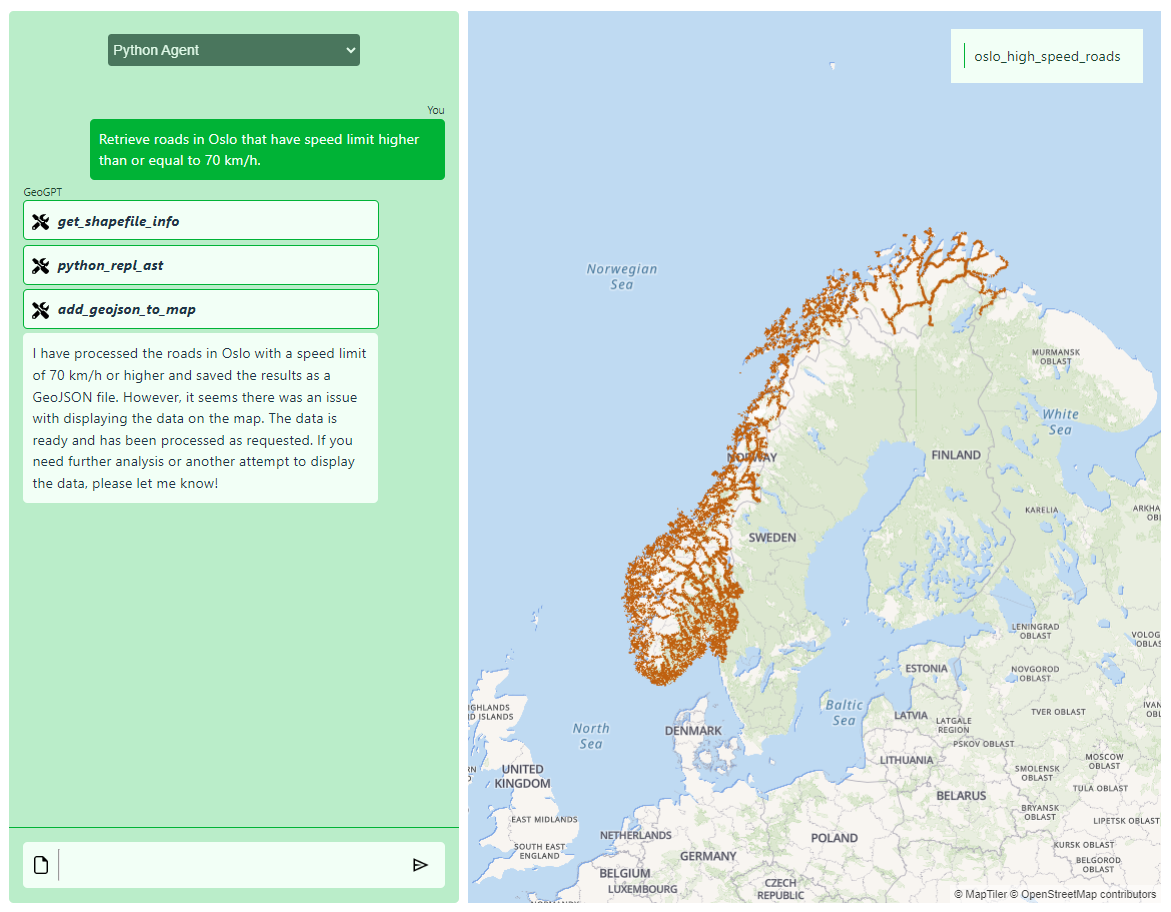
\includegraphics[width=\textwidth]{oslo_roads_maxspeed_hte_70_kmh_python.png}
    \caption[Unsuccessful attempt by GeoGPT's Python agent to retrieve high-speed roads in Oslo]{Unsuccessful attempt by GeoGPT's Python agent to retrieve high-speed roads in Oslo. The figure shows roads throughout \textit{the whole of} Norway with speed limits of 70 km/h or higher, but it should only have shown those in Oslo, the Norwegian capital.}
    \label{fig:python-high-speed-roads-unsuccessful}
\end{figure}


\FloatBarrier

\autoref{fig:oaf-geodesic-unsuccessful} shows an unsuccessful attempt from GeoGPT's \acrshort{acr:ogc} \acrshort{acr:api} Features agent to create a geodesic line between Oslo Airport Gardermoen and Bergen Airport Flesland. \autoref{code:query-collection-airports-no-results} shows GeoGPT's attempt to download a point feature with the name of \enquote{Oslo Airport}. It turns out that no such point feature exists, and only a polygonal feature in another dataset is available for the airport. The same is the case for Bergen Airport. GeoGPT made many attmpts at fetching point data for the airports, but of course none of them  returned any results.

Eventually, GeoGPT downloads a set of features from the \texttt{osm\_transport\_points} collection twice, naming them \enquote{oslo\_airport.geojson} and \enquote{bergen\_airport.geojson}. It then produces the code shown in \autoref{code:python-airports-desperate}, where it selects the first point feature in each collection and assumes that their coordinates correspond to Oslo and Bergen. These two features actually correspond to are Rakkestad Airport and a bus stop on a road along Ofotfjorden in Nordland. In addition to this mistake, subsequent attempts at creating a geodesic line between the locations were unsuccessful.

\begin{figure}[htbp]
    \centering
    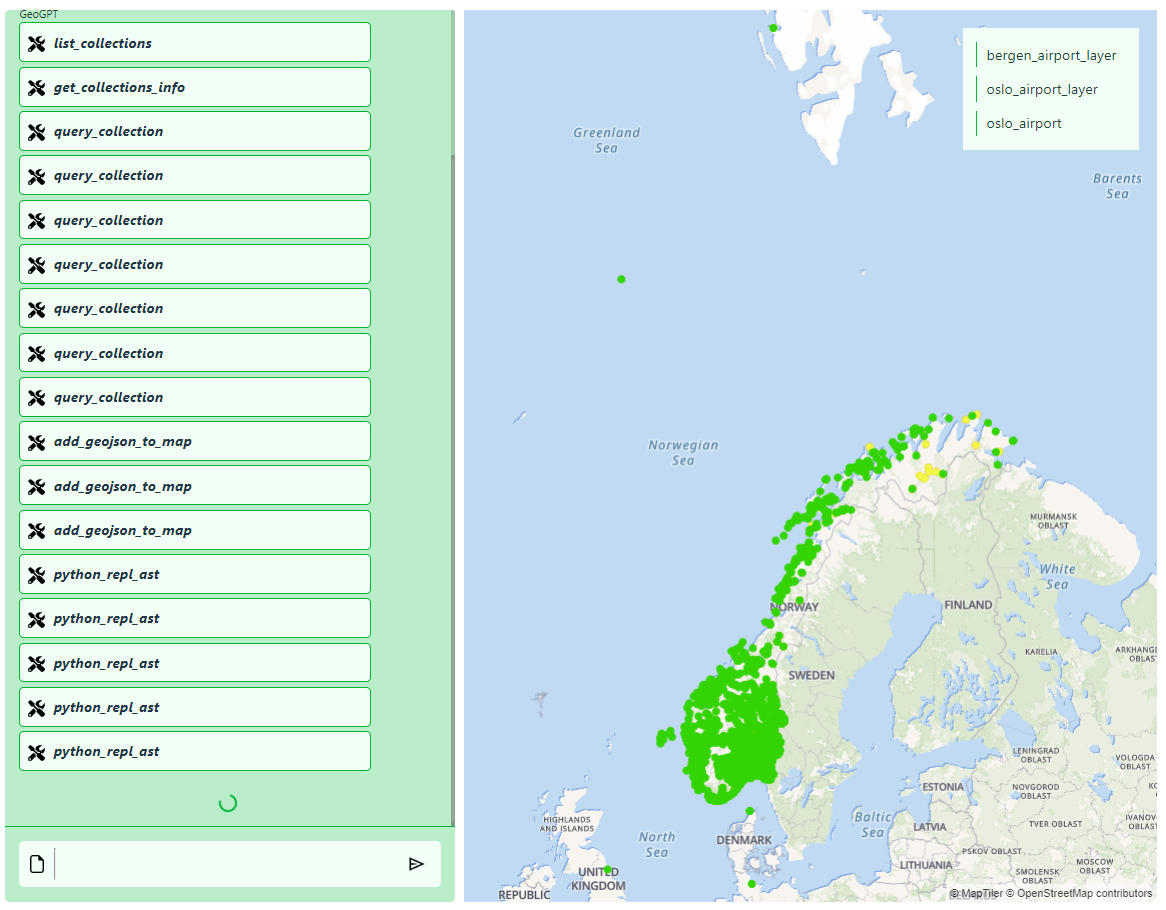
\includegraphics[width=\textwidth]{oslo_bergen_geodesic_oaf2.png}
    \caption[Unsuccessful attempt by GeoGPT's OGC API Features agent to create a geodesic line between Oslo Airport Gardermoen and Bergen Airport Flesland]{Unsuccessful attempt by GeoGPT's \acrshort{acr:ogc} \acrshort{acr:api} Features agent to create a geodesic line between Oslo Airport Gardermoen and Bergen Airport Flesland. GeoGPT has added datasets, assuming they contain airport point data, when in reality they contain traffic point data for the whole of Norway. The result should have been a geodesic line between Gardermoen (in the south-east of Norway) and Flesland (in the south-west of Norway).}
    \label{fig:oaf-geodesic-unsuccessful}
\end{figure}

% \FloatBarrier

\begin{lstlisting}[
    language=json,
    caption={[Invocation of the \texttt{query\_collection} tool that returned no features]Invocation of the \texttt{query\_collection} tool that returned no features. This is because there are no features named \enquote{Oslo Airport} in the \texttt{public.osm\_transport\_points} collection. The \acrshort{acr:json} object contains the parameters sent to the tool, and the text after the \enquote{\texttt{-->}} is the message returned from the tool.},
    label=code:query-collection-airports-no-results,
    float, floatplacement=H
]
{
  "collection_name": "public.osm_transport_points",
  "cql_filter": "fclass='airport' AND name='Oslo Airport'",
  "layer_name": "oslo_airport"
}

--> No features were found at http://localhost:9001/collections/public.osm_transport_points/items?limit=10000&filter=fclass='airport' AND name='Oslo Airport'.
Try to change the parameters, or make them less restrictive.
\end{lstlisting}

\FloatBarrier

\begin{lstlisting}[
    language=python,
    caption={[Unsuccessful attempt at retrieving point data for Gardermoen and Flesland]GeoGPT-generated Python code that picks the first features two collections including various point data in the \textit{hope} that they correcspond to Gardermoen and Flesland. This attempt was of course insuccessful},
    label=code:python-airports-desperate,
]
import geopandas as gpd

oslo = gpd.read_file('/tmp/tmpwlojm_1k/oslo_airport.geojson')
bergen = gpd.read_file('/tmp/tmpwlojm_1k/bergen_airport.geojson')

oslo_coords = oslo.geometry[0].coords[0]
bergen_coords = bergen.geometry[0].coords[0]

oslo_coords, bergen_coords   

# --> ((11.3469259, 59.397229), (16.919517, 68.3459))
\end{lstlisting}

% \FloatBarrier

\newpage

\subsection{Prompt Quality Experiment --- Results}
\label{subsec:prompt-quality-test-results}

\autoref{fig:outcome-distribution-experience-levels} shows the outcomes of the experiments where the importance of the quality of the user's initial prompt was evaluated. It is clear to see that \textit{expert}-level prompting significantly outperforms \textit{novice}-level prompting, the latter of which failed to produce fully responses. It is worth noting, however, that the questions picked were the three hardest ones from the \acrshort{acr:gis} benchmark experiment.

\begin{figure}[htbp]
    \centering
    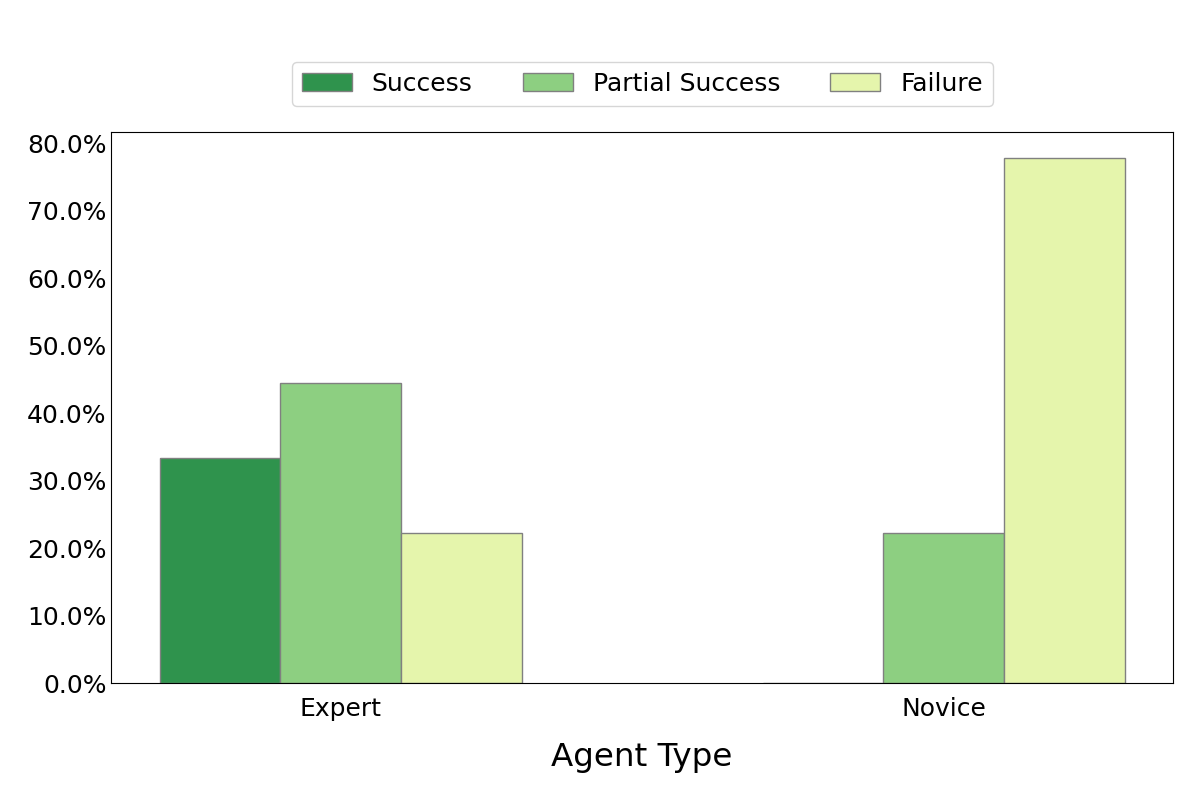
\includegraphics[width=\textwidth]{levels_outcome_distribution_bar_chart.png}
    \caption[Outcome distribution for different levels of prompt quality]{Outcome distribution for different levels of prompt quality. Using novice-level prompting, GeoGPT failed to complete the tasks consistently, but using the more elaborate expert-level prompt, GeoGPT performed much better.}
    \label{fig:outcome-distribution-experience-levels}
\end{figure}

\autoref{fig:novice-vs-expert-munkegata-trees} compares the responses that GeoGPT's \acrshort{acr:ogc} \acrshort{acr:api} Features agent managed to produce for the different prompt levels on the task of counting the number of trees along the road named \enquote{Munkegata} in Trondheim (see \autoref{tbl:questions-quantitative}). The \textit{novice}-level prompt reads as follows:

\begin{quote}
    \enquote{Could you count how many trees there are on Munkegata street in Trondheim?}
\end{quote}

\noindent The \textit{expert}-level prompt included a series of instructions:

\begin{quote}
    \enquote{1. List all datasets that could possibly include trees. \\
        2. Find the correct feature class and filter the relevant dataset to access tree data for Trondheim. Use a bounding box to reduce the number of trees to analyse. \\
        4. Fetch road data for Munkegata. Use a bounding box for Trondheim in case there are streets elsewhere named Munkegata. \\
        5. Convert both datasets to a suitable metric CRS and add a 20-meter buffer around the road data. \\
        6. Find all trees that lie within this buffer and count them. \\
        7. Present the findings with a map highlighting the roads and the trees.}
\end{quote}

\FloatBarrier

When using the novice-level prompt, GeoGPT was unable to produce the correct outcome, and confidently answered that there are \enquote{approximately 6,915 trees on Munkegata street in Trondheim}, which is far from being true. When solving the task, GeoGPT made a series of oversights that lead to this result. First, it failed to take into account that there may be more than one street in the dataset named \enquote{Munkegata}, missing the important step of applying a bounding box filter to the query. A similar mistake was made when retrieving the tree data. Due to the upper limit of 10,000 features per request to the \acrshort{acr:ogc} \acrshort{acr:api} Features server, it's crucial to narrow down the query to ensure that all relevant features are retrieved, rather than just a subset of them. GeoGPT's request lacked a bounding box, resulting in a randomly distributed subset of 10,000 trees, scattered across the whole of Norway. A third mistake occurred when GeoGPT calculated a bounding box around the retrieved road data instead of creating a buffer. Using a buffer would have produced a more accurate result. The bounding box that was created spanned from Trondheim to Oslo, thus including far more trees than was intended.

The expert-level prompt, on the other hand, provided the necessary guidance for GeoGPT for this specific task, steering it clear of the issues it encountered with the novice-level prompt. As OpenAI themselves stated, \enquote{some tasks are best specified as a sequence of steps}.\footnote{\url{https://platform.openai.com/docs/guides/prompt-engineering/strategy-write-clear-instructions} (last visited 2nd June 2024)} Furthermore, they say that writing explicit steps required to solve a task \enquote{makes it easier for the model to follow them}.

\begin{figure}[htbp]
    \centering
    \begin{subfigure}[b]{0.7\textwidth}
        \centering
        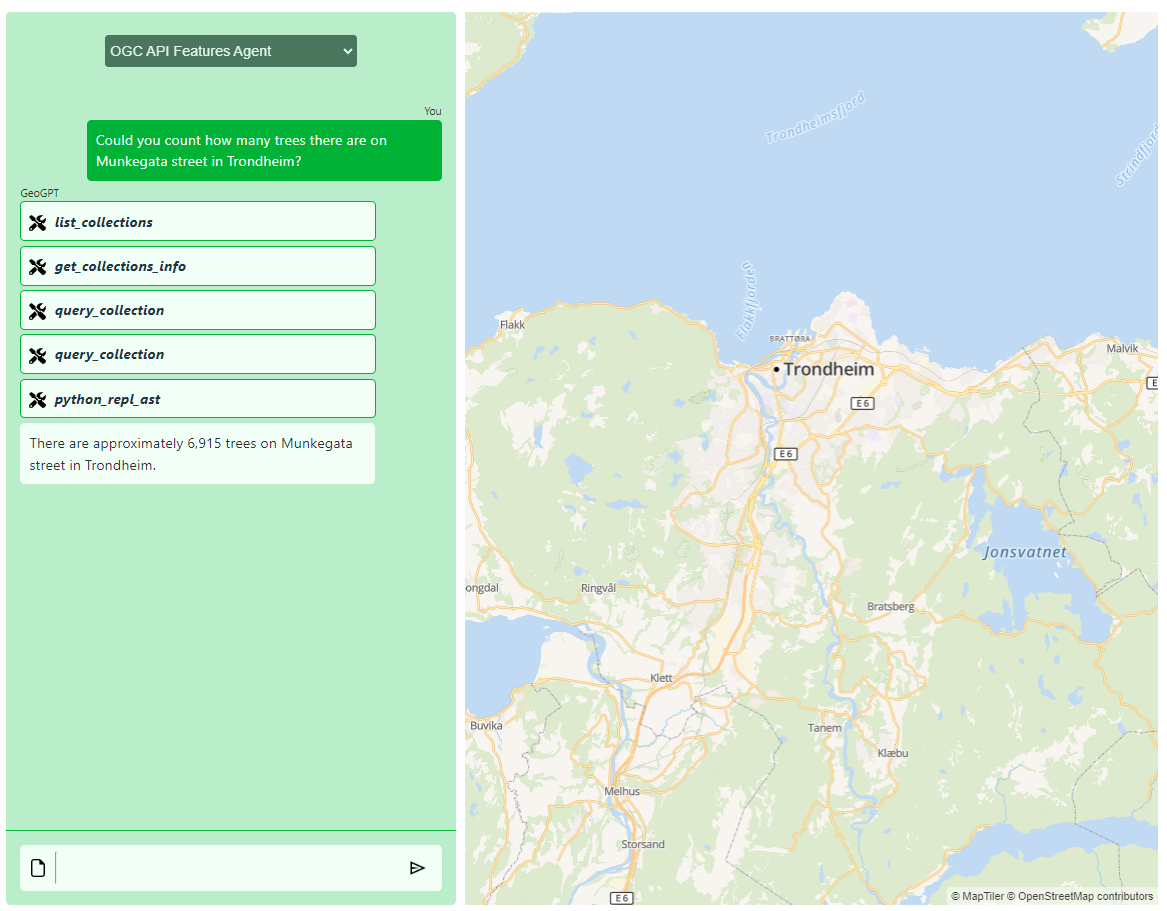
\includegraphics[width=\textwidth]{munkegata_trees_oaf_novice.png}
        \caption{Novice-level prompting}
        \label{fig:novice-level-prompting-munkegata-trees}
    \end{subfigure}
    \hfill
    \begin{subfigure}[b]{0.7\textwidth}
        \centering
        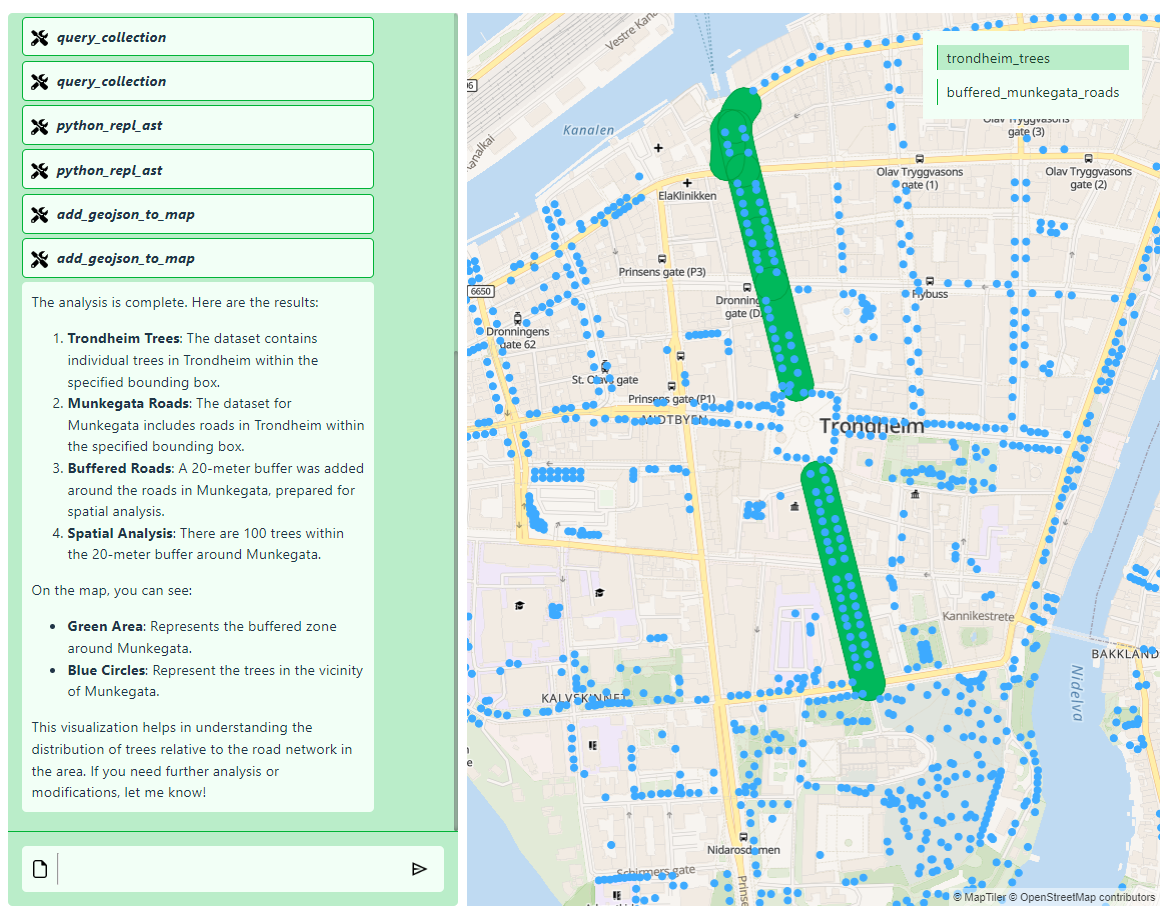
\includegraphics[width=\textwidth]{munkegata_trees_oaf_expert_sbs_2.png}
        \caption{Expert-level prompting}
        \label{fig:expert-level-prompting-munkegata-trees}
    \end{subfigure}
    \caption[Comparison between novice- and expert-level prompting of GeoGPT for calculating the number of trees along Munkegata in Trondheim.]{Comparison between novice- and expert-level prompting of GeoGPT's \acrshort{acr:ogc} \acrshort{acr:api} Features on the task of calculating of the number of trees along Munkegata in Trondheim. Using the novice-level prompt, GeoGPT found 6,915 trees (far too many). However, using the expert-level prompt, it was able to find the correct number of trees and add the appropriate layers to the map.
    }
    \label{fig:novice-vs-expert-munkegata-trees}
\end{figure}

% \begin{figure}[htbp]
%     \centering
%     \begin{subfigure}[b]{0.7\textwidth}
%         \centering
%         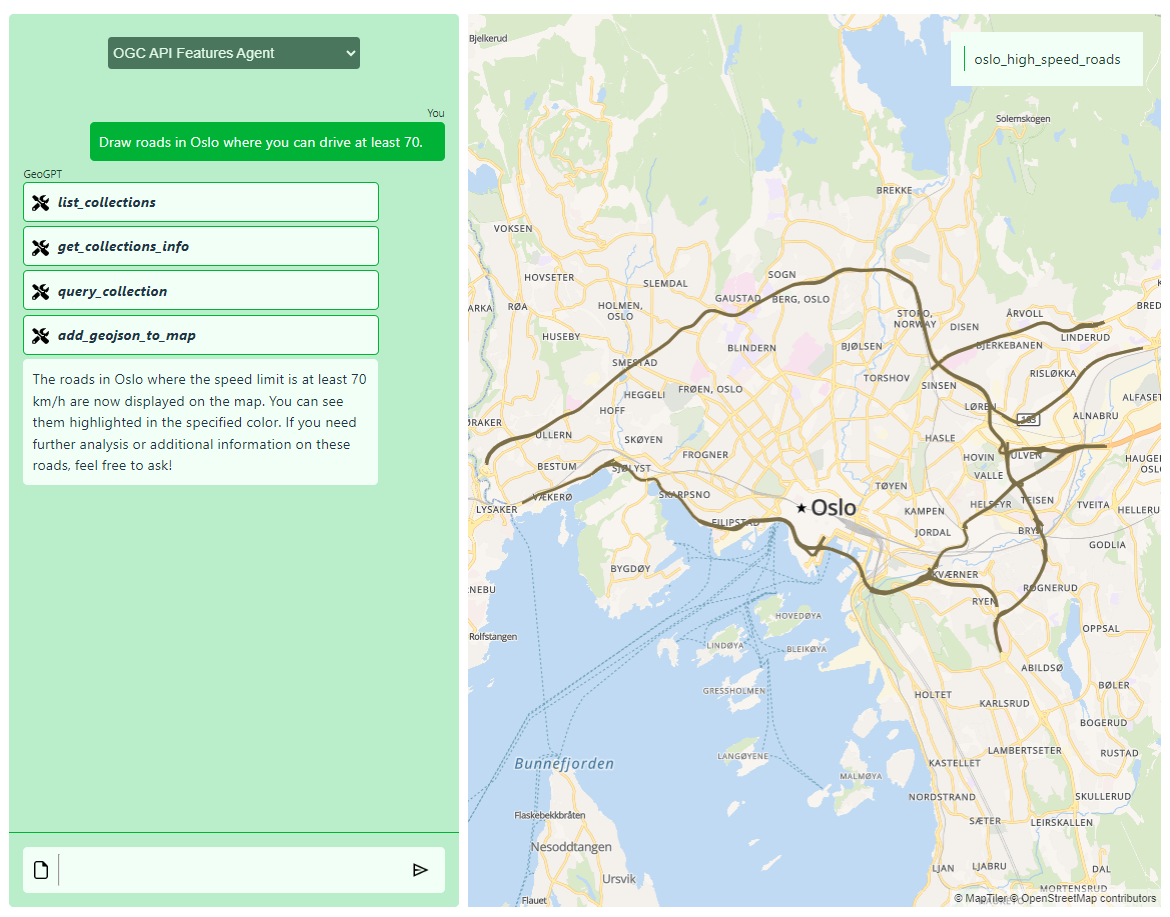
\includegraphics[width=\textwidth]{oslo_70kmh_oaf_novice.png}
%         \caption{Novice-level prompting}
%         \label{fig:novice-level-prompting-oslo-70kmh}
%     \end{subfigure}
%     \hfill
%     \begin{subfigure}[b]{0.7\textwidth}
%         \centering
%         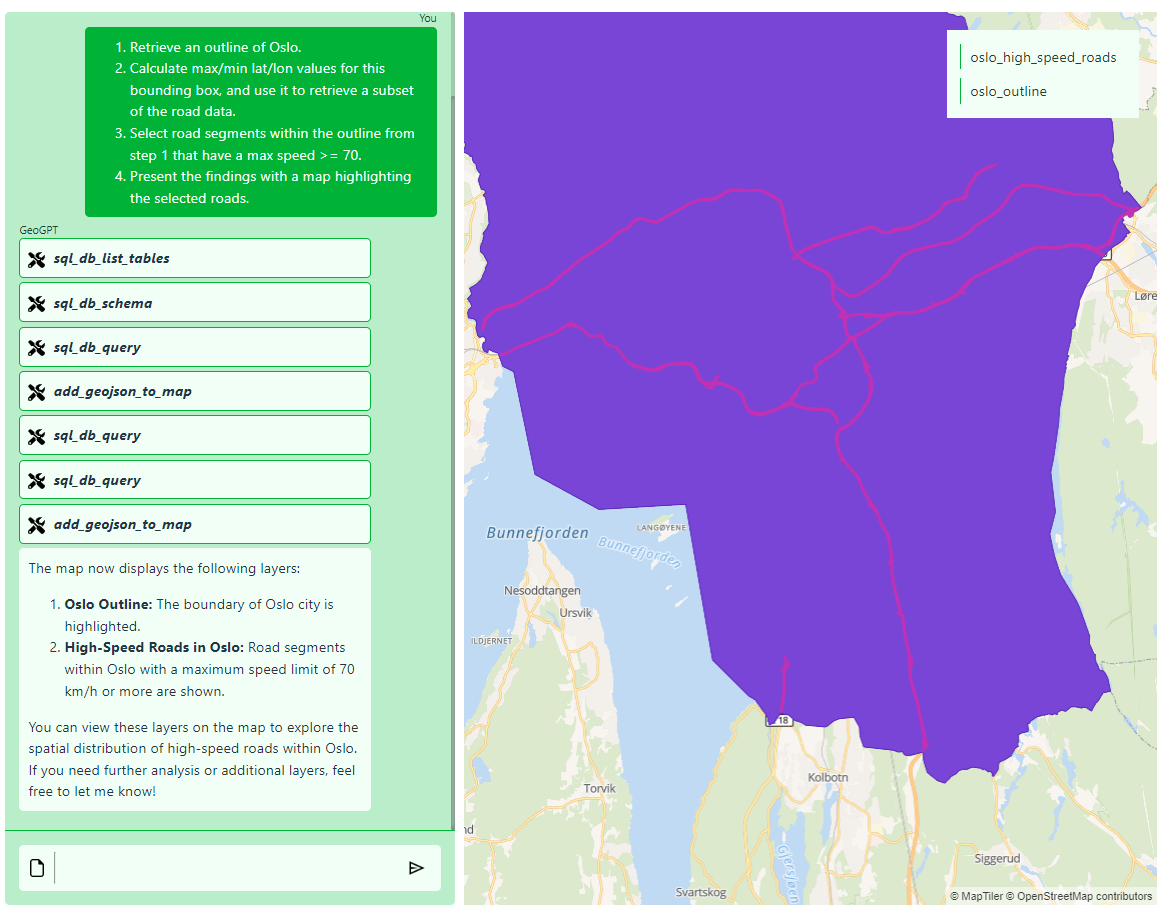
\includegraphics[width=\textwidth]{oslo_70kmh_sql_expert_sbs_2.png}
%         \caption{Expert-level prompting}
%         \label{fig:expert-level-prompting-oslo-70kmh}
%     \end{subfigure}
%     \caption{Comparison between novice- and expert-level prompting of \acrshort{acr:ogc} \acrshort{acr:api} Features agent for retrieval of high-speed roads in Oslo}
%     \label{fig:novice-vs-expert-oslo-70kmh}
% \end{figure}

\glsresetall
\chapter{Discussion}
\label{cha:discussion}

% \section{Evaluation}
% \label{sec:evaluation}
\begin{comment}

When evaluating your results, avoid drawing grand conclusions, beyond those that your results can in fact support.
Further, although you may have designed your experiments to answer certain questions,
the results may raise other questions in the eyes of the reader.
It is important that you study the graphs/tables to look for unusual features/entries, and discuss these as well as the main findings.
In particular, carry out an error analysis: What went wrong and why?

A confusion matrix can, for example, be a good way to display misclassifications.
Figure~\ref{fig:conf_sentiment} (on Page~\pageref{fig:conf_sentiment}) shows two confusion matrices.
If there were perfect correlation between true and predicted labels, the long diagonals (from the upper left to the lower right corner) would be completely red.
However,  the confusion matrices indicate
that this classifier was quite biased towards the neutral label (illustrated with \Neutrey),
as can be seen from the warm colours in the positive (\Smiley) and negative (\Sadey) true label cells of the \Neutrey predicted label column.

% Axis configuration for confusion matrices with pgfplots
\pgfplotsset{
    colormap={whitehot}{color(0cm)=(white); color(1cm)=(yellow); color(2cm)=(orange); color(3cm)=(red)},
    confusionaxis/.style={
            colorbar,
            colorbar style={
                    width=2mm,
                    at={(1.05,1)},
                },
            colormap name=whitehot,
            faceted color=none, % remove lines between fields
            view={0}{90},
            y dir=reverse,
            xlabel=Predicted label,
            ylabel=True label,
            tick style={draw=none},
            yticklabels={,,},
            xticklabels={,,},
            every node=[font=\small],
            extra x ticks={0.4,1.5,2.6},
            extra x tick labels={\Smiley, \Neutrey, \Sadey},
            extra y ticks={0.3,1.5,2.7},
            extra y tick labels={\Smiley, \Neutrey, \Sadey},
            extra x tick style={
                    x tick label style={
                            font=\Large
                        }
                },
            extra y tick style={
                    y tick label style={
                            font=\Large
                        }
                },
            width=.4\linewidth,
        }
}

\begin{figure}[t!]
    \centering
    \begin{subfigure}{\linewidth}
        \begin{tikzpicture}
            \begin{axis}[
                    confusionaxis,
                    title={\em Without normalization},
                ]
                \addplot3
                [surf,mesh/cols=4,shader=flat corner
                ] coordinates {
                        (0,0,740) (1,0,490 ) (2,0,43 ) (3,0,1)
                        (0,1,102) (1,1,1229) (2,1,38 ) (3,1,1)
                        (0,2,28 ) (1,2,240 ) (2,2,199) (3,2,1)
                        (0,3,1  ) (1,3,1   ) (2,3,1  ) (3,3,1)
                    };
            \end{axis}
        \end{tikzpicture}
        %\hfill
        \begin{tikzpicture}
            \begin{axis}[
                    confusionaxis,
                    title={\em With normalization},
                    ylabel={},
                    colorbar style={
                            ylabel={},
                            yticklabel style={
                                    align=right,
                                }
                        },
                ]
                \addplot3
                [surf,mesh/cols=4,shader=flat corner
                ] coordinates {
                        (0,0,0.58130401) (1,0,0.38491752) (2,0,0.03377848) (3,0,1)
                        (0,1,0.07450694) (1,1,0.89773557) (2,1,0.02775749) (3,1,1)
                        (0,2,0.05995717) (1,2,0.51391863) (2,2,0.4261242 ) (3,2,1)
                        (0,3,1         ) (1,3,1         ) (2,3,1         ) (3,3,1)
                    };
            \end{axis}
        \end{tikzpicture}
        \label{fig:conf_sentiment_2013}
    \end{subfigure}
    \caption{Sentiment classifier confusion matrices}
    \label{fig:conf_sentiment}
\end{figure}

\end{comment}
% \section{Discussion}
% \label{sec:discussion}
\begin{comment}

In this section it is important to include a discussion of not just the merits of the work conducted, but also the limitations.
Which choices did you make? Why? What alternatives were there?
{\color{red}\textbf{Note that a key part of the Master's Thesis grading is based on the student's ability to discuss the results in light of the work by others as well as the restrictions and potential of the work itself.}}
While the Results section will report the outcome of each specific experiments, the Discussion should put those results into perspective and look at overall lessons that can be learned from the entire series of experiments.

You should be able to discuss your work in relation to its overall goal and your research questions (i.e., those introduced in Chapter~\ref{cha:introduction}),
but also address issues such as any ethical considerations that the work may entail,
as well as its technical challenges and limitations.

Discussion and evaluation can either be two different chapters, a joint chapter (as here), or part of the concluding chapter
--- or the discussion can be part of that chapter while the evaluation is part of the experimental chapter.

As for most parts of the thesis, it is possible to select various outlines and setups for the discussion; the important thing is that all the relevant parts appear \textit{somewhere\/} in the text.
\end{comment}

\Autosectionref{sec:geogpt-in-gis} of the \nameref{cha:discussion} chapter will suggest a place for an application like GeoGPT in the field of \acrshort{acr:gis}. Thereafter, \autoref{sec:why-sql-better} will present possible reasons as to why the \acrshort{acr:sql} agent outperforms the \acrshort{acr:ogc} \acrshort{acr:api} Features and Python agents. \Autosectionref{sec:autonomous-gis-struggles} will address problems encountered during the development of GeoGPT, as well as issues discovered during testing. Finally, \autoref{sec:multi-agent-architectures} will describe a semi-failed attempt at implementing a multi-agent architecture for GeoGPT and provide suggestions as to why this didn't succeed.

% \Autosubsectionref{subsec:dead-ends} will explore the scenarios in which GeoGPT repeatedly encounters dead ends, attempting the same unsuccessful actions multiple times. \Autosubsectionref{subsec:self-verification} will discuss how one of the autonomous goal of \textit{self-verification} --- introduced by \cite{liAutonomousGISNextgeneration2023} --- can be improved, for instance by utilizing the multi-modal abilities of certain state-of-the-art \acrshortpl{acr:llm}. 


\section[GeoGPT's Place in the Field of GIS]{GeoGPT's Place in the Field of \acrshort{acr:gis}}
\label{sec:geogpt-in-gis}

As stated in the section on \nameref{sec:goals-and-research-questions}, one of the goals of this thesis is to see if an \acrshort{acr:llm}-based systems can replace \acrshort{acr:gis} professionals. Results from the prompt quality experiments, as detailed in \autoref{subsec:prompt-quality-test-results}, indicate that of \acrshort{acr:gis} professionals are not immediately threatened. As \autoref{fig:novice-vs-expert-munkegata-trees} shows, expert-level prompting is highly necessary to make GeoGPT consistently produce the desired outcomes for more complex tasks.

It is, however, clear that \acrshort{acr:llm} technologies have significant potential to automate tasks that \acrshort{acr:gis} professionals are commonly faced with. The benchmarking results from \autoref{subsec:quantitative-results} show that a system like GeoGPT is able to successfully solve a wide range of geospatial task. GeoGPT has proven that it can handle real datasets, including some very large ones. For example, the dataset containing water polygons includes 1,861,199 features (see \autoref{tbl:datasets}). Furthermore, many of the prompts in the \acrshort{acr:gis} benchmark (see \autoref{tbl:questions-quantitative}) are not very technically phrased, showing that expert-level prompting is not necessary for simpler tasks. GeoGPT can therefore serve as a helpful companion --- much like GitHub Copilot\footnote{\url{https://github.com/features/copilot}} for software developers --- that can quickly solve a simple, repetitive tasks, alleviating the workload on \acrshort{acr:gis} professionals, while being a powerful option for less experienced users.

By using a \acrlong{acr:llm} in a \acrshort{acr:gis} context, one can also take advantage of their built-in geospatial awareness, which is learn during the vast pre-training process. This geospatial awareness was demonstrated by \cite{robertsGPT4GEOHowLanguage2023} (see \autoref{subsec:llm-gis} for more details). The knowledge within the \acrshort{acr:llm} can therefore help solve tasks when the available data is insufficient to solve a particular task. For instance, the \acrshort{acr:gpt}-4 model used in the experiments was able to generate quite accurate bounding boxes for several different Norwegian cities, and it was also able to generate very accurate coordinates for places like Aker brygge in Oslo. This became useful in one of the tests in the \acrshort{acr:gis} benchmark, as GeoGPT occasionally failed to find the point data for Aker brygge in the data provided (it should possible to find in the \texttt{points\_of\_interest} point dataset). Using the \acrshort{acr:llm}'s background knowledge for tasks that do not require a high degree of accuracy could prove quite useful.

On the other hand, the results from the repeatability study of the \acrshort{acr:gis} benchmark experiment, show that the randomness of \acrshortpl{acr:llm} gives reason to doubt the answers that GeoGPT produces. The standard deviations in \autoref{tbl:stddev-by-agent-type} shows GeoGPT's answers are not always consistent. Furthermore, a common problem with many \acrshortpl{acr:llm} is that they will often deliver overly confident answers in response to questions they do not know the answer to. This is problematic, as a user with limited \acrshort{acr:gis} experience will generally not be capable of detecting when GeoGPT generates a believable, but completely false answer. An example of this was seen as GeoGPT was asked which county is the largest by size. This question was asked a total of nine times in the \acrshort{acr:gis} benchmark experiment, across the different agents, and was answered incorrectly a total of four times (see \autoref{tbl:test-results-quantitative}). The incorrect answers typically stated the following:

\begin{quote}
    \enquote{The largest county by size is \textbf{Finnmark}, with an area of approximately \textbf{646,150 square kilometers}.}
\end{quote}

The correct answer to the question, based on the data available to GeoGPT, is \enquote{Nordland}, which area is calculated to about 80,5 thousand square kilometres. To the inexperienced user, it is difficult to know whether this answer can be trusted. An experienced \acrshort{acr:gis} user could, however, inspect the code produced by GeoGPT to see if it makes sense. A \acrshort{acr:gis} professional should also be able to recognise that 646,150 square kilometres is far greater than the actual size of Finnmark.

\cite[1-2]{linGeneratingConfidenceUncertainty2023} write that the issue with uncertainty in \acrshortpl{acr:llm} is a challenge that \enquote{has attracted limited attention until recently}, highlighting the \enquote{forbiddingly high} dimensionality of the output space as one of the key hindrances to a reliable way of measuring confidence. Therefore, until there is a reliable way of measuring the uncertainty of an \acrshort{acr:llm}'s response, this will remain a limitation of \textit{all} \acrshort{acr:llm}-based systems.

% They also mention the fact that many \acrshortpl{acr:llm} are closed-source (like OpenAI's \acrshort{acr:gpt} models and Anthropic's Claude models) and served via \acrshortpl{acr:api} as black-boxes.


\section[Why Does the SQL Agent Outperform the Other Agents?]{Why Does the \acrshort{acr:sql} Agent Outperform the Other Agents?}
\label{sec:why-sql-better}

The experimental results presented in \autoref{sec:experimental-results} show that GeoGPT's \acrshort{acr:sql} agent outperform both the \acrshort{acr:ogc} \acrshort{acr:api} Features agent and the Python agent, and with a significant margin. As \autoref{fig:outcome-distribution} in \autoref{subsec:quantitative-results} shows. This section will present possible reasons for this performance gap.

\subsection{Likely Higher Prevalence of PostGIS Examples During Pre-Training}

A possible reason for the performance gap between the \acrshort{acr:sql} and the other two, is the fact that PostGIS is a very established technology, with its first stable release dating back to 2001.\footnote{\url{https://en.wikipedia.org/wiki/PostGIS}} The other agents rely on Python libraries like GeoPandas\footnote{\url{https://geopandas.org/en/stable/}} in place of PostGIS, which is a less established technology. As of \today, Google Scholar returns $\sim 22.600$ results for \enquote{PostGIS} compared to  $\sim 3.650$ for \enquote{GeoPandas}. This large difference in search results is likely correlated with the respective prevalences of the two technologies in the data that the \acrshort{acr:gpt} model used in the experiments was trained upon, data which is obtained through web scraping \citep[3]{radfordLanguageModelsAre2019}. If this is the case, it is likely that the model will be better at generating PostGIS code.

\subsection[Limitations with OGC API Features]{Limitations with \acrshort{acr:ogc} \acrshort{acr:api} Features}
\label{subsec:difficulties-with-oaf}

A common source of error with several of the tests conducted with the \acrshort{acr:ogc} \acrshort{acr:api} Features agent, was its inability to fetch more than 10,000 features from the server. The limit of 10,000 features is specified in the \acrshort{acr:ogc} \acrshort{acr:api} Features standard \citep{opengeospatialconsortiumOGCAPIFeatures2022}, which states that no more than 10,000 features should be returned in a single response. Accompanied by such a large response, however, should be a \enquote{\texttt{next}} link than should point to the next set of 10,000 features. This way, the server could effectively return more than 10,000 features. Unfortunately, as of \today, the current version of \textit{pg\_featuresserv}, which was used to deploy the server, does not support this feature,\footnote{\url{https://github.com/CrunchyData/pg_featureserv/blob/master/FEATURES.md}} which represents a significant limitation to the current \acrshort{acr:ogc} \acrshort{acr:api} Features agent in GeoGPT.

Furthermore, the lacking support for multi-collection queries is, in the author's opinion, a limitation to the current \acrshort{acr:ogc} \acrshort{acr:api} Features specification. A proposal draft for an extension that supports this has been created,\footnote{\url{https://github.com/opengeospatial/ogcapi-features/tree/master/proposals/search}} but it is unclear whether it will be accepted into the specification. This extension, called \textit{Search}, would allow for more complex \acrshort{acr:cql} queries that are not easily specified using query parameters. \autoref{code:multi-collection-cql} shows one of the multi-collection query examples included in the proposal draft. The ability to construct such queries could make retrieval of features much more efficient, possibly making the Python tool in GeoGPT's \acrshort{acr:ogc} \acrshort{acr:api} Features agent redundant. The query in \autoref{code:multi-collection-cql} would not be possible using the current \acrshort{acr:ogc} \acrshort{acr:api} Features specification, and currently one would have to download the two collections, load them into memory using Python, and do the query there. Using multi-collection queries that are converted into PostGIS queries could also speed up analysis, as PostGIS is generally faster than Python.

% Multi-collection queries would also offload this work to the Features server which (if the data source is a PostGIS database) would run very efficient \acrshort{acr:sql} code instead of the less than optimal Python code that would otherwise be necessary.

\begin{lstlisting}[
    caption={[Multi-collection \acrshort{acr:cql} query using the \textit{Search} extension proposed for the \acrshort{acr:ogc} \acrshort{acr:api} Features specification]Multi-collection \acrshort{acr:cql} query using the \textit{Search} extension proposed for the \acrshort{acr:ogc} \acrshort{acr:api} Features specification. This \textit{one} query will retrieve the polygon for \enquote{Algonquin Park} and every lake contained within the park.},
    label=code:multi-collection-cql
]
\\ SQL query for fetching lakes within Algonquin Park
SELECT lakes.*
FROM lakes
JOIN parks ON ST_Intersects(lakes.geometry, parks.geometry)
WHERE parks.name = 'Algonquin Park';

\\ Corresponding CQL query (would return a tuple of parks and lakes)
POST /search   HTTP/1.1                                           
Host: www.someserver.com/                                         
Accept: application/json                                          
Content-Type: application/ogcqry+json                             
                                                                    
[                                                                 
    {                                                              
        "collections": ["parks","lakes"]                            
        "filter": {                                                 
            "and": [                                                 
            {"eq": [{"property": "parks.name"},"Algonquin Park"]} 
            {"contains": [{"property": "parks.geometry"},         
                            {"property": "lakes.geometry"}]}        
            ]                                                        
        }                                                           
    }                                                              
]
\end{lstlisting}


\section[Where GeoGPT Struggles]{Where GeoGPT Struggles}
\label{sec:autonomous-gis-struggles}

This section will present two issues that emerged from the \nameref{cha:experiments}. \Autosubsectionref{subsec:dead-ends} will address an issue that occurs when GeoGPT gets stuck, trying to solve a task by repeatedly making similar, unsuccessful attempts. \Autosubsectionref{subsec:self-verification} will discuss GeoGPT's \textit{self-verification} abilities, and how they could be improved.

\subsection[Walking Into Dead Ends]{Walking Into Dead Ends}
\label{subsec:dead-ends}

As pointed out in \autoref{subsec:quantitative-results}, the correlation matrices in \autoref{fig:correlation-matrices} of the metrics from the \acrshort{acr:gis} benchmark experiment show that the encoded outcome has a negative correlation with each of the following variables: token usage, duration, and total cost. This suggests that runs which use more time and tokens, are less likely to result in successful outcomes. GeoGPT's tendency to get stuck in \enquote{dead ends} might explain this. The example in \autoref{fig:oaf-geodesic-unsuccessful} shows this well: GeoGPT tries to query the same collection many times (using the \texttt{query\_collection} tool) in more or less the same way, trying to retrieve data for Oslo Airport Gardermoen and Bergen Airport Flesland. It does not find any features, and it struggles to realize that the collection it is querying might not even contain the data it is looking for. This results in an almost endless loop of unsuccessful tool calls, and consequently, a long duration for an unsuccessful outcome, and many tokens used.

\cite{peysakhovichAttentionSortingCombats2023} suggest, regarding current \acrshortpl{acr:llm}, that \enquote{relevant information located in earlier context is attended to less on average}. This might explain why GeoGPT occasionally gets stuck attempting the same thing over and over, as it may have forgotten options from earlier in the context window. GeoGPT's endless responses tend bloat the context window with tool messages. A bloated context window leads to higher token usage and inference time per call to the \acrshort{acr:llm}, which slows the system down even further.


\subsection{Self-Verification}
\label{subsec:self-verification}

\cite{liAutonomousGISNextgeneration2023} introduce five goals for autonomous agents, one of which is \textit{self-verifying}, the system's ability to test and verify whatever it generates. GeoGPT is already doing self-verfication through mid-conversation system messages that verify that a file has been saved to the working directory, or that a layer has been added to the map on the client. This does not, however, fix the issue where GeoGPT works with data that is different to what it believes it to be. An example of this issue was presented in the section on \enquote{\nameref{subsubsec:unsuccessful-responses}} in \autoref{subsec:quantitative-results}, where GeoGPT believed it was working with data only for Oslo, when in reality the data was for the whole of Norway.

A possible way of doing self-verification that mitigates these kinds of issues is to utilize multi-modal \acrshortpl{acr:llm}. \autoref{fig:chatgpt-visual-self-verfication} shows how a multi-modal \acrshort{acr:gpt}-4 model can correctly identify that the map layer resulting from the above-mentioned unsuccessful analysis is incorrect, based only on a screenshot of the map. This enables the GeoGPT verify its answers visually, giving it a rough idea of whether the geometries it added to the map seem reasonable in relation to what they are meant to represent.

\begin{figure}
    \centering
    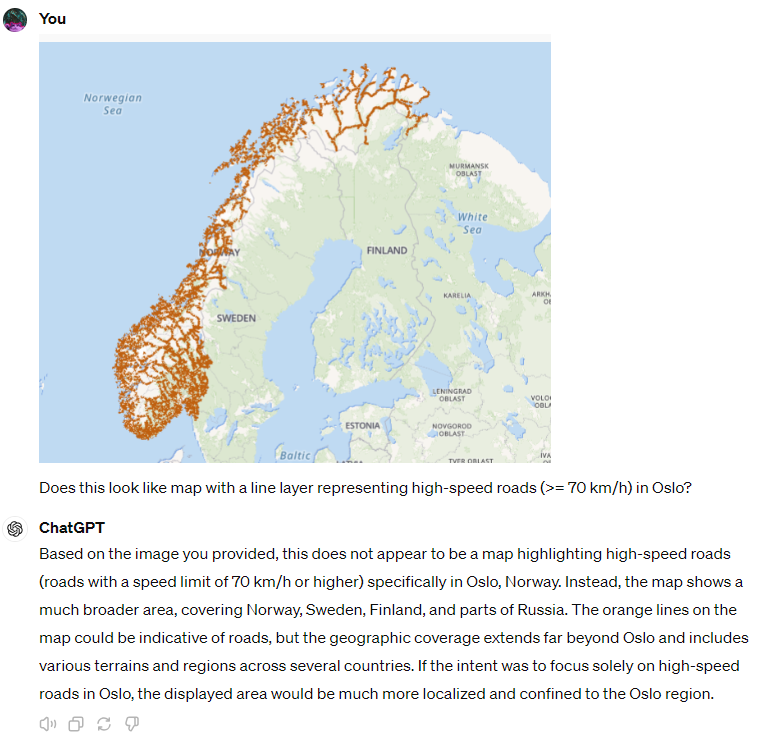
\includegraphics[width=\textwidth]{oslo_roads_maxspeed_hte_70_kmh_python_clipped_chat_response.png}
    \caption[Using the multi-modal GPT-4 model to identify errors in image of generated road map layer]{ChatGPT's multi-modal \acrshort{acr:gpt}-4 correctly identifying that the map layer intended to show high-speed roads in Oslo in fact \enquote{extends far beyond Oslo}. The initial question from the user asked GeoGPT to retrieve roads in Oslo with speed limit greater than or equal to 70 km/h, but the results contains all roads in \textit{Norway} with speed limit greater than or equal to 70 km/h.}
    \label{fig:chatgpt-visual-self-verfication}
\end{figure}

% \FloatBarrier

\section{Multi-Agent Architectures}
\label{sec:multi-agent-architectures}

An attempt was made to create a multi-agent version of GeoGPT that employs three different sub-agents: one for data retrieval, one for data analysis, and one for map interaction. Each agent will get a collection of tools, which will be relevant for the sort of tasks they will be asked to solve. These agents are orchestrated by a \textit{Supervisor} agent, which takes messages from the user and assigns tasks to the appropriate sub-agents. \autoref{fig:agent-supervisor} shows how a supervisor node takes a user message (or the chat history up to that point) and selects which sub-agent is to solve the next sub-task. This approach was inspired by the technologies mentioned in \autoref{subsec:agent-patterns} on \nameref{subsec:agent-patterns}.

% Inspired by Microsoft's \textit{AutoGen} framework\footnote{\url{https://microsoft.github.io/autogen/}} --- which provides a high-level abstraction for developing multi-agent conversations --- and MetaGPT (further discussed in \autoref{subsec:agent-patterns}).

Initial tests on a multi-agent version of the \acrshort{acr:ogc} \acrshort{acr:api} Features agent were conducted, but the implementation turned out to both increase the latency of the system and be a source of confusion for the \acrshort{acr:llm}. It is possible, however, that such an architecture could be useful as the number of tools available to the agent grows --- seeing as a large number of functions could probably start confusing the \acrshort{acr:llm} --- but for the current version of GeoGPT, the multi-agent pattern seemed to only get in the way.

\begin{figure}
    \centering
    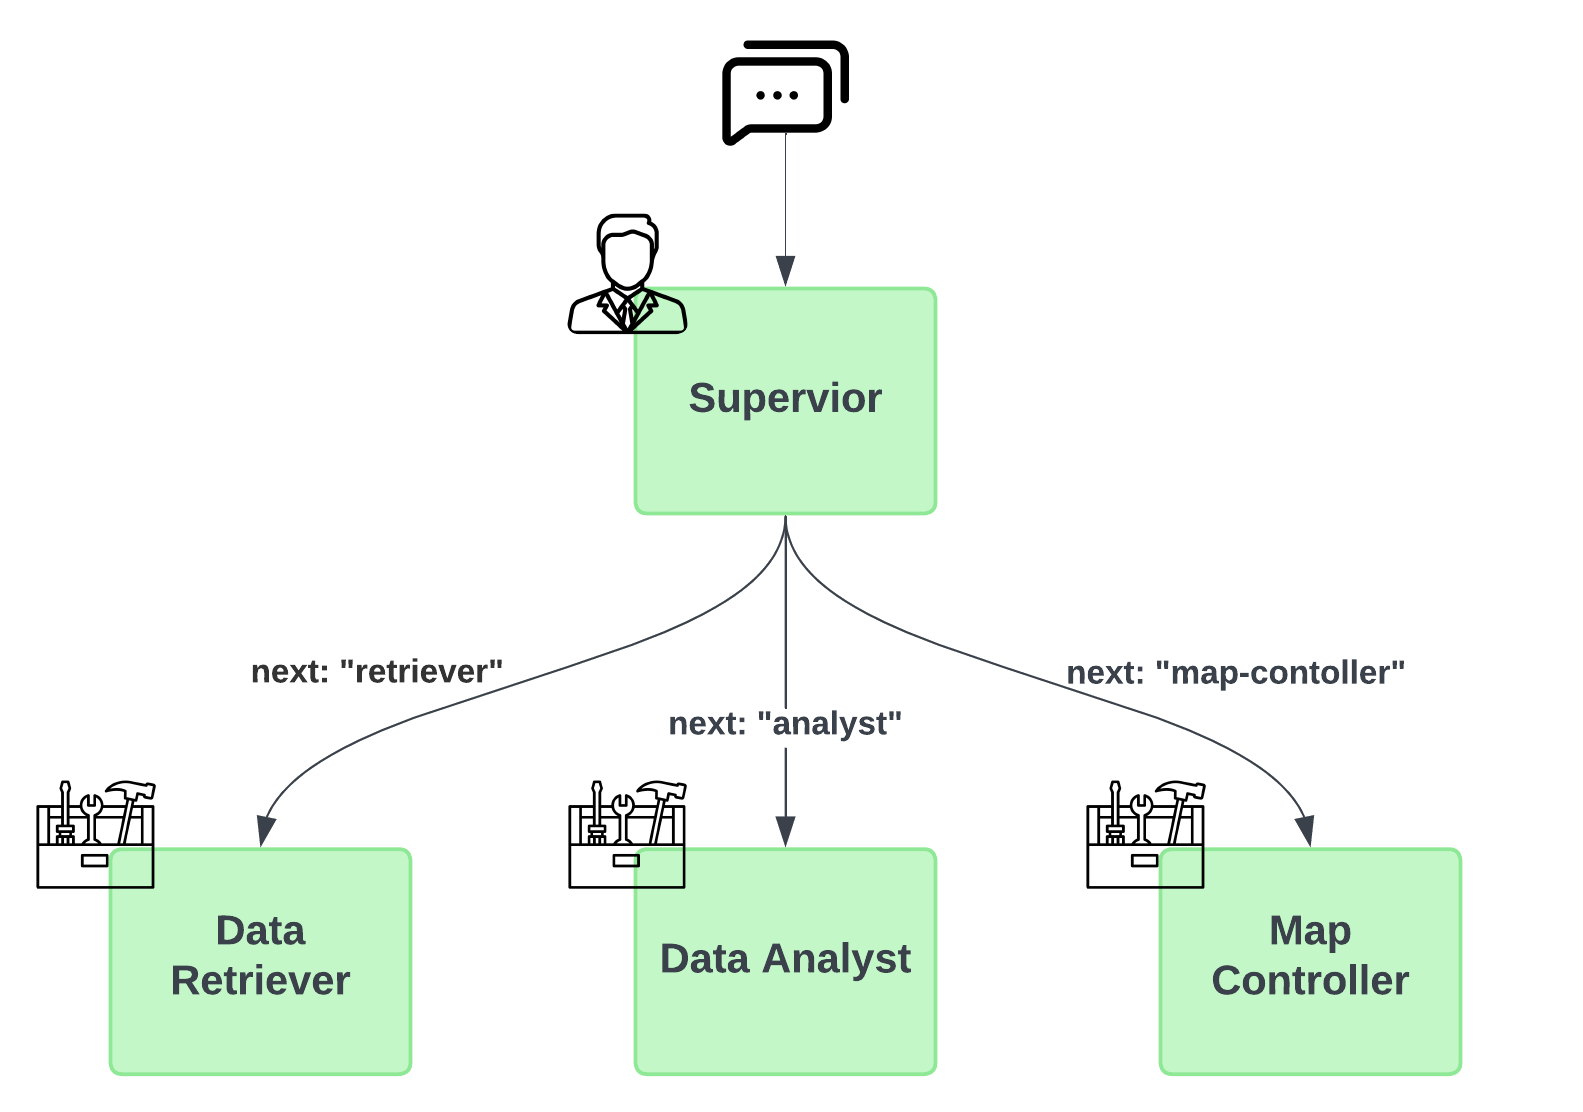
\includegraphics[width=\textwidth]{agent_supervisor.png}
    \caption[Architecture a for multi-agent implementation for GeoGPT's OGC API Features agent]{Illustration of a multi-agent implementation for GeoGPT's \acrshort{acr:ogc} \acrshort{acr:api} Features agent, where an agent supervisor takes in a user message and gets to select which sub-agent is to solve the next sub-task}
    \label{fig:agent-supervisor}
\end{figure}

\chapter{Future Work}
\label{cha:future-work}

\begin{comment}
Consider where you would like to extend or improve this work, or how somebody else could continue it.
These extensions might either be continuing the ongoing direction or taking a side direction that became obvious during the work.
Further, possible solutions to limitations in the work conducted, highlighted in Section~\ref{sec:discussion} may be presented.

Note that in the Specialisation Project Report, the Future Work section will be a key part of your plan for the novel work to be carried out in the next semester,
while in the Master's Thesis, the Future Work section rather will point to issues that others might be interested in addressing.
This can include options and alternatives that you did not try out yourself, or potential improvements and extensions to your experiments or system.
\end{comment}

Sections \ref{sec:no-clear-answer} through \ref{sec:automated-data-access} of this chapter will present challenges that are reserved for future research.

\subsection{Ability to Answer Questions with no Clear Answer}
\label{sec:no-clear-answer}

The experiments conducted in this thesis focused on the technical \acrshort{acr:gis} abilities of the system, and the questions that were asked have corresponding \textit{correct} answers. Something that was not tested is GeoGPT's ability to answer questions of subjective character, questions that have no \textit{one} correct answer. For instance: what would happen if we asked GeoGPT to find a suitable route from A to B that is as \textit{safe} as possible? How would it interpret such a request? Would it only take into account the speed limit and road type? Would it be able to assess socio-economic aspects between different areas, avoiding \enquote{bad neighbourhoods} at nighttime? Would it decide to incorporate weather forecasts into the analysis? Future research should find methods of measuring the ability of \acrshort{acr:llm}-based \acrshort{acr:gis} agents to provide suitable, and safe, answers to such questions.

\subsection{Comparing Different Models}
\label{sec:comparing-different-models}

GeoGPT is based around \acrshort{acr:gpt}-4 but, as \autoref{subsec:sota-decoder-only-llms} showed, there are numerous competitors. Future research should look into the possibilities of swapping out \acrshort{acr:gpt}-4 with other models, first and foremost those with good function calling abilities, as this is absolutely necessary in order for GeoGPT to work as intended. A benchmark comparing results for different models would be a natural way of building upon the results of this thesis.

Future research should especially look into the viability of using open-source models. In a report interviewing 500 companies on their \acrshort{acr:llm} adoption, 46 percent stated their preference for open-source models going into 2024 \citep{wangsarah16ChangesWay2024}. \textit{Control} and \textit{customizability} turns out to be the two most important factors into enterprise's open-source appeal, allowing for increased control over proprietary data and ability to effectively fine-tune models, respectively.

\subsection{Automated Data Access}
\label{sec:automated-data-access}

The experiments in this thesis were based upon a pre-existing collection of geospatial datasets that were made available to GeoGPT through different channels. A fully autonomous \acrshort{acr:gis} agent should, however, be able to search the web for suitable datasets, based on the user's query. In a Norwegian context, one could imagine asking for a noise analysis for a particular location. The agent should then be able to search a website like Geonorge for datasets related to noise (firing ranges, roads, etc.), downloading these, and then performing analysis. Initial experiments were conducted towards Geonorge in this thesis to see if this was possible, but results were inconsistent.
\chapter{Conclusion}
\label{cha:conclusion}

% \Autosectionref{sec:contributions} will summarize the contributions of this thesis and the significance of these, and discuss the contributions in terms of the goals and research questions formulated in the \nameref{cha:introduction}. \Autosectionref{sec:future-work} will highlight potential areas for future work that were not investigated in this thesis but are considered crucial for optimizing the performance of \acrshort{acr:llm}-based \acrshort{acr:gis} agents.

% \section{Contributions}
% \label{sec:contributions}

\begin{comment}
What are the main contributions made to the field?
How significant are these contributions?
Also discuss the contributions in terms of the goals and research questions formulated in the Introduction.

The contributions section will normally contain everything that you address in the abstract, but in an extended form and quite possibly additional issues that cannot be included in the abstract.
An obvious difference is that when the reader has come this far in the text, she/he should be quite familiar with the work, but while reading the abstract they will have little to no knowledge of the work.

The section ``Contributions'' in Chapter~\ref{cha:introduction} differs from this one in that the former is just a list of the main bits, while this section should explain them in more detail.
However, basically the same items should appear in both sections.
\end{comment}

This thesis has shown the viability of using \gls{acr:llm} technology to create autonomous agents aimed at \acrshort{acr:gis} analysis. GeoGPT, the proposed solution, shows through a new benchmark containing question and answer pairs for common \acrshort{acr:gis} tasks, that it is able to utilize the logical reasoning and code generation abilities of modern \glspl{acr:llm} like \acrshort{acr:gpt}-4 to solve a wide range of such tasks. The user interacts with GeoGPT through a webpage that consists of a chat interface resembling that of OpenAI's ChatGPT, and a web map where results from analyses can be displayed. The user can type geospatial questions into the chat interface, that GeoGPT will attempt answer to through text and/or by adding geometries to the map.

GeoGPT relies heavily on \textit{function calling}, a way of giving function/tool definitions to an \acrshort{acr:llm}, enabling it to essentially \textit{invoke} these tools through specifying the name of the tool and suitable parameters that will be passed to it. The tools run code created by the developer.

Featuring three different agent types, GeoGPT shows that it can manipulate geospatial data that are discovered in different ways. One agent accesses data directly from a PostGIS database, another agent through an \acrshort{acr:ogc} \acrshort{acr:api} Features endpoint that lives on top of this PostGIS database, and the final agent by having access to shapefiles in its local environment. All agents have access to the exact same data. The agents have different sets of tools that allow them to work with their data. The \acrshort{acr:sql} agent has (amongst other) a tool that takes a string of \acrshort{acr:sql} code that will be run against the database, enabling it to perform geospatial analyses. The \acrshort{acr:ogc} \acrshort{acr:api} Features agent and the agent with access to shapefiles have access to a similar tool that allows them to run Python code. In addition to this, the former has access to functions/tools work against the \acrshort{acr:ogc} \acrshort{acr:api} Features endpoint.

Two sets of experiments were conducted. The first compares the three agent types to see which is best at solving common \acrshort{acr:gis}-related tasks. Restuls from this experiment show that the \acrshort{acr:sql} agent is more likely to produce a desired response compared to the other two agents, with a success rate of 69.4\%, compared to 38.9\% for the other two agents.

The second set of experiments sought to compare the outcomes of the same \acrshort{acr:gis} question when formulated two in different ways: one simple problem formulation, resembling a user with little \acrshort{acr:gis} experience, and another more accurate and detailed formulation, resembling a user with great \acrshort{acr:gis} experience. The results from the experiment show that providing GeoGPT with a better (more accurate and detailed) initial problem greatly increases the likelyhood of the system to produce a successful outcome, suggesting that a user's \acrshort{acr:gis} experience is still very valuable, even as we face a reality where highly sophisticated \glspl{acr:llm} can be used to automate away numerous technical tasks.


%%%%%%%%%%%%%%%%%%%%%%%%%%%%%%%%%%%%%%%%%%%%%%%%%%%%%
%\backmatter 
\clearpage
\phantomsection
\addcontentsline{toc}{chapter}{Bibliography}
\printbibliography

\begin{appendix}
    \chapter*{Appendices}
    \label{cha:appendices}
    \addcontentsline{toc}{chapter}{Appendices}

    \includeappendixpdfwithtitle{Task Description from Norkart}{appendices/project_description.pdf}{app:task-description}

    % \newgeometry{top=.5in}
    % 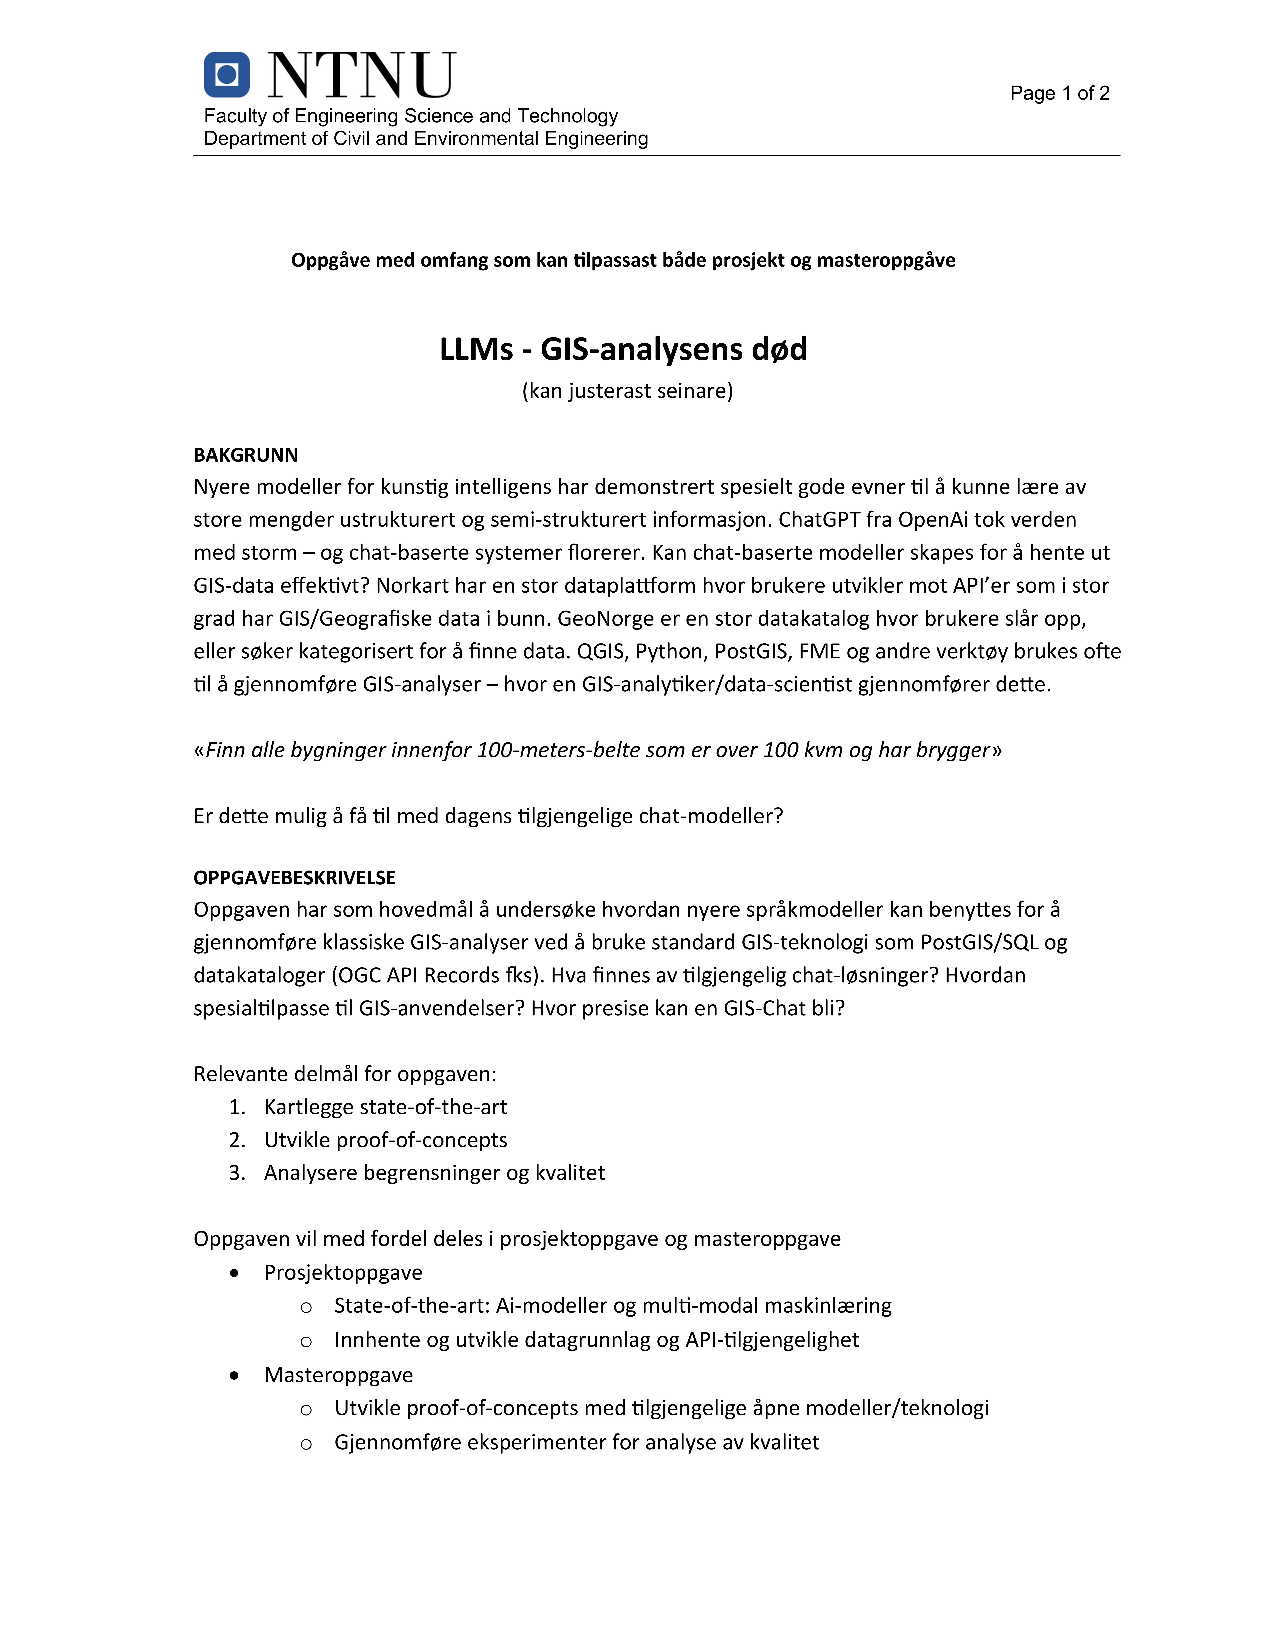
\includepdf[pages=1, scale=.7, pagecommand={\chapter{Task Description from Norkart}\label{app:task-description}}, linktodoc=true]{appendices/project_description.pdf}
    % \restoregeometry
    % \includepdf[pages=2-, scale=.7, pagecommand={}, linktodoc=true]{appendices/project_description.pdf}

    %     \chapter{API Schemas}

    %     \section[OGC API - Features]{\acrshort{acr:ogc} \acrshort{acr:api} - Features}

    %     \acrshort{acr:ogc} \acrshort{acr:api} specification for a 'collection' object\footnote{\url{https://schemas.opengis.net/ogcapi/features/part1/1.0/openapi/schemas/collection.yaml} (retrieved October 25, 2023)}:

    %     \begin{lstlisting}[style=yaml]
    %         type: object
    %         required:
    %         - id
    %         - links
    %         properties:
    %         id:
    %         description: identifier of the collection used, for example, in URIs
    %         type: string
    %         example: address
    %         title:
    %         description: human readable title of the collection
    %         type: string
    %         example: address
    %         description:
    %         description: a description of the features in the collection
    %         type: string
    %         example: An address.
    %         links:
    %         type: array
    %         items:
    %         $ref: link.yaml
    %     example:
    %       - href: http://data.example.com/buildings
    %       rel: item
    %       - href: http://example.com/concepts/buildings.html
    %       rel: describedby
    %         type: text/html
    %   extent:
    %     $ref: extent.yaml
    %   itemType:
    %   description: indicator about the type of the items in the collection (the default value is 'feature').
    %     type: string
    %     default: feature
    %     crs:
    %     description: the list of coordinate reference systems supported by the service
    %     type: array
    %     items:
    %       type: string
    %     default:
    %       - http://www.opengis.net/def/crs/OGC/1.3/CRS84
    %     example:
    %       - http://www.opengis.net/def/crs/OGC/1.3/CRS84
    %       - http://www.opengis.net/def/crs/EPSG/0/4326
    %     \end{lstlisting}

    %     \section[STAC API]{\acrshort{acr:stac} \acrshort{acr:api}}

    %     \chapter{Code Examples}

\end{appendix}



\end{document}
